%%%%%%%% ICML 2025 EXAMPLE LATEX SUBMISSION FILE %%%%%%%%%%%%%%%%%

\documentclass{article}

% Recommended, but optional, packages for figures and better typesetting:
\usepackage{microtype}
\usepackage{graphicx}
\usepackage{subfigure}
\usepackage{booktabs} % for professional tables

% hyperref makes hyperlinks in the resulting PDF.
% If your build breaks (sometimes temporarily if a hyperlink spans a page)
% please comment out the following usepackage line and replace
% \usepackage{icml2025} with \usepackage[nohyperref]{icml2025} above.
\usepackage{hyperref}


% Attempt to make hyperref and algorithmic work together better:
\newcommand{\theHalgorithm}{\arabic{algorithm}}

% Use the following line for the initial blind version submitted for review:
% \usepackage{icml2025}

% If accepted, instead use the following line for the camera-ready submission:
\usepackage[accepted]{icml2025}



%
\setlength\unitlength{1mm}
\newcommand{\twodots}{\mathinner {\ldotp \ldotp}}
% bb font symbols
\newcommand{\Rho}{\mathrm{P}}
\newcommand{\Tau}{\mathrm{T}}

\newfont{\bbb}{msbm10 scaled 700}
\newcommand{\CCC}{\mbox{\bbb C}}

\newfont{\bb}{msbm10 scaled 1100}
\newcommand{\CC}{\mbox{\bb C}}
\newcommand{\PP}{\mbox{\bb P}}
\newcommand{\RR}{\mbox{\bb R}}
\newcommand{\QQ}{\mbox{\bb Q}}
\newcommand{\ZZ}{\mbox{\bb Z}}
\newcommand{\FF}{\mbox{\bb F}}
\newcommand{\GG}{\mbox{\bb G}}
\newcommand{\EE}{\mbox{\bb E}}
\newcommand{\NN}{\mbox{\bb N}}
\newcommand{\KK}{\mbox{\bb K}}
\newcommand{\HH}{\mbox{\bb H}}
\newcommand{\SSS}{\mbox{\bb S}}
\newcommand{\UU}{\mbox{\bb U}}
\newcommand{\VV}{\mbox{\bb V}}


\newcommand{\yy}{\mathbbm{y}}
\newcommand{\xx}{\mathbbm{x}}
\newcommand{\zz}{\mathbbm{z}}
\newcommand{\sss}{\mathbbm{s}}
\newcommand{\rr}{\mathbbm{r}}
\newcommand{\pp}{\mathbbm{p}}
\newcommand{\qq}{\mathbbm{q}}
\newcommand{\ww}{\mathbbm{w}}
\newcommand{\hh}{\mathbbm{h}}
\newcommand{\vvv}{\mathbbm{v}}

% Vectors

\newcommand{\av}{{\bf a}}
\newcommand{\bv}{{\bf b}}
\newcommand{\cv}{{\bf c}}
\newcommand{\dv}{{\bf d}}
\newcommand{\ev}{{\bf e}}
\newcommand{\fv}{{\bf f}}
\newcommand{\gv}{{\bf g}}
\newcommand{\hv}{{\bf h}}
\newcommand{\iv}{{\bf i}}
\newcommand{\jv}{{\bf j}}
\newcommand{\kv}{{\bf k}}
\newcommand{\lv}{{\bf l}}
\newcommand{\mv}{{\bf m}}
\newcommand{\nv}{{\bf n}}
\newcommand{\ov}{{\bf o}}
\newcommand{\pv}{{\bf p}}
\newcommand{\qv}{{\bf q}}
\newcommand{\rv}{{\bf r}}
\newcommand{\sv}{{\bf s}}
\newcommand{\tv}{{\bf t}}
\newcommand{\uv}{{\bf u}}
\newcommand{\wv}{{\bf w}}
\newcommand{\vv}{{\bf v}}
\newcommand{\xv}{{\bf x}}
\newcommand{\yv}{{\bf y}}
\newcommand{\zv}{{\bf z}}
\newcommand{\zerov}{{\bf 0}}
\newcommand{\onev}{{\bf 1}}

% Matrices

\newcommand{\Am}{{\bf A}}
\newcommand{\Bm}{{\bf B}}
\newcommand{\Cm}{{\bf C}}
\newcommand{\Dm}{{\bf D}}
\newcommand{\Em}{{\bf E}}
\newcommand{\Fm}{{\bf F}}
\newcommand{\Gm}{{\bf G}}
\newcommand{\Hm}{{\bf H}}
\newcommand{\Id}{{\bf I}}
\newcommand{\Jm}{{\bf J}}
\newcommand{\Km}{{\bf K}}
\newcommand{\Lm}{{\bf L}}
\newcommand{\Mm}{{\bf M}}
\newcommand{\Nm}{{\bf N}}
\newcommand{\Om}{{\bf O}}
\newcommand{\Pm}{{\bf P}}
\newcommand{\Qm}{{\bf Q}}
\newcommand{\Rm}{{\bf R}}
\newcommand{\Sm}{{\bf S}}
\newcommand{\Tm}{{\bf T}}
\newcommand{\Um}{{\bf U}}
\newcommand{\Wm}{{\bf W}}
\newcommand{\Vm}{{\bf V}}
\newcommand{\Xm}{{\bf X}}
\newcommand{\Ym}{{\bf Y}}
\newcommand{\Zm}{{\bf Z}}

% Calligraphic

\newcommand{\Ac}{{\cal A}}
\newcommand{\Bc}{{\cal B}}
\newcommand{\Cc}{{\cal C}}
\newcommand{\Dc}{{\cal D}}
\newcommand{\Ec}{{\cal E}}
\newcommand{\Fc}{{\cal F}}
\newcommand{\Gc}{{\cal G}}
\newcommand{\Hc}{{\cal H}}
\newcommand{\Ic}{{\cal I}}
\newcommand{\Jc}{{\cal J}}
\newcommand{\Kc}{{\cal K}}
\newcommand{\Lc}{{\cal L}}
\newcommand{\Mc}{{\cal M}}
\newcommand{\Nc}{{\cal N}}
\newcommand{\nc}{{\cal n}}
\newcommand{\Oc}{{\cal O}}
\newcommand{\Pc}{{\cal P}}
\newcommand{\Qc}{{\cal Q}}
\newcommand{\Rc}{{\cal R}}
\newcommand{\Sc}{{\cal S}}
\newcommand{\Tc}{{\cal T}}
\newcommand{\Uc}{{\cal U}}
\newcommand{\Wc}{{\cal W}}
\newcommand{\Vc}{{\cal V}}
\newcommand{\Xc}{{\cal X}}
\newcommand{\Yc}{{\cal Y}}
\newcommand{\Zc}{{\cal Z}}

% Bold greek letters

\newcommand{\alphav}{\hbox{\boldmath$\alpha$}}
\newcommand{\betav}{\hbox{\boldmath$\beta$}}
\newcommand{\gammav}{\hbox{\boldmath$\gamma$}}
\newcommand{\deltav}{\hbox{\boldmath$\delta$}}
\newcommand{\etav}{\hbox{\boldmath$\eta$}}
\newcommand{\lambdav}{\hbox{\boldmath$\lambda$}}
\newcommand{\epsilonv}{\hbox{\boldmath$\epsilon$}}
\newcommand{\nuv}{\hbox{\boldmath$\nu$}}
\newcommand{\muv}{\hbox{\boldmath$\mu$}}
\newcommand{\zetav}{\hbox{\boldmath$\zeta$}}
\newcommand{\phiv}{\hbox{\boldmath$\phi$}}
\newcommand{\psiv}{\hbox{\boldmath$\psi$}}
\newcommand{\thetav}{\hbox{\boldmath$\theta$}}
\newcommand{\tauv}{\hbox{\boldmath$\tau$}}
\newcommand{\omegav}{\hbox{\boldmath$\omega$}}
\newcommand{\xiv}{\hbox{\boldmath$\xi$}}
\newcommand{\sigmav}{\hbox{\boldmath$\sigma$}}
\newcommand{\piv}{\hbox{\boldmath$\pi$}}
\newcommand{\rhov}{\hbox{\boldmath$\rho$}}
\newcommand{\upsilonv}{\hbox{\boldmath$\upsilon$}}

\newcommand{\Gammam}{\hbox{\boldmath$\Gamma$}}
\newcommand{\Lambdam}{\hbox{\boldmath$\Lambda$}}
\newcommand{\Deltam}{\hbox{\boldmath$\Delta$}}
\newcommand{\Sigmam}{\hbox{\boldmath$\Sigma$}}
\newcommand{\Phim}{\hbox{\boldmath$\Phi$}}
\newcommand{\Pim}{\hbox{\boldmath$\Pi$}}
\newcommand{\Psim}{\hbox{\boldmath$\Psi$}}
\newcommand{\Thetam}{\hbox{\boldmath$\Theta$}}
\newcommand{\Omegam}{\hbox{\boldmath$\Omega$}}
\newcommand{\Xim}{\hbox{\boldmath$\Xi$}}


% Sans Serif small case

\newcommand{\Gsf}{{\sf G}}

\newcommand{\asf}{{\sf a}}
\newcommand{\bsf}{{\sf b}}
\newcommand{\csf}{{\sf c}}
\newcommand{\dsf}{{\sf d}}
\newcommand{\esf}{{\sf e}}
\newcommand{\fsf}{{\sf f}}
\newcommand{\gsf}{{\sf g}}
\newcommand{\hsf}{{\sf h}}
\newcommand{\isf}{{\sf i}}
\newcommand{\jsf}{{\sf j}}
\newcommand{\ksf}{{\sf k}}
\newcommand{\lsf}{{\sf l}}
\newcommand{\msf}{{\sf m}}
\newcommand{\nsf}{{\sf n}}
\newcommand{\osf}{{\sf o}}
\newcommand{\psf}{{\sf p}}
\newcommand{\qsf}{{\sf q}}
\newcommand{\rsf}{{\sf r}}
\newcommand{\ssf}{{\sf s}}
\newcommand{\tsf}{{\sf t}}
\newcommand{\usf}{{\sf u}}
\newcommand{\wsf}{{\sf w}}
\newcommand{\vsf}{{\sf v}}
\newcommand{\xsf}{{\sf x}}
\newcommand{\ysf}{{\sf y}}
\newcommand{\zsf}{{\sf z}}


% mixed symbols

\newcommand{\sinc}{{\hbox{sinc}}}
\newcommand{\diag}{{\hbox{diag}}}
\renewcommand{\det}{{\hbox{det}}}
\newcommand{\trace}{{\hbox{tr}}}
\newcommand{\sign}{{\hbox{sign}}}
\renewcommand{\arg}{{\hbox{arg}}}
\newcommand{\var}{{\hbox{var}}}
\newcommand{\cov}{{\hbox{cov}}}
\newcommand{\Ei}{{\rm E}_{\rm i}}
\renewcommand{\Re}{{\rm Re}}
\renewcommand{\Im}{{\rm Im}}
\newcommand{\eqdef}{\stackrel{\Delta}{=}}
\newcommand{\defines}{{\,\,\stackrel{\scriptscriptstyle \bigtriangleup}{=}\,\,}}
\newcommand{\<}{\left\langle}
\renewcommand{\>}{\right\rangle}
\newcommand{\herm}{{\sf H}}
\newcommand{\trasp}{{\sf T}}
\newcommand{\transp}{{\sf T}}
\renewcommand{\vec}{{\rm vec}}
\newcommand{\Psf}{{\sf P}}
\newcommand{\SINR}{{\sf SINR}}
\newcommand{\SNR}{{\sf SNR}}
\newcommand{\MMSE}{{\sf MMSE}}
\newcommand{\REF}{{\RED [REF]}}

% Markov chain
\usepackage{stmaryrd} % for \mkv 
\newcommand{\mkv}{-\!\!\!\!\minuso\!\!\!\!-}

% Colors

\newcommand{\RED}{\color[rgb]{1.00,0.10,0.10}}
\newcommand{\BLUE}{\color[rgb]{0,0,0.90}}
\newcommand{\GREEN}{\color[rgb]{0,0.80,0.20}}

%%%%%%%%%%%%%%%%%%%%%%%%%%%%%%%%%%%%%%%%%%
\usepackage{hyperref}
\hypersetup{
    bookmarks=true,         % show bookmarks bar?
    unicode=false,          % non-Latin characters in AcrobatÕs bookmarks
    pdftoolbar=true,        % show AcrobatÕs toolbar?
    pdfmenubar=true,        % show AcrobatÕs menu?
    pdffitwindow=false,     % window fit to page when opened
    pdfstartview={FitH},    % fits the width of the page to the window
%    pdftitle={My title},    % title
%    pdfauthor={Author},     % author
%    pdfsubject={Subject},   % subject of the document
%    pdfcreator={Creator},   % creator of the document
%    pdfproducer={Producer}, % producer of the document
%    pdfkeywords={keyword1} {key2} {key3}, % list of keywords
    pdfnewwindow=true,      % links in new window
    colorlinks=true,       % false: boxed links; true: colored links
    linkcolor=red,          % color of internal links (change box color with linkbordercolor)
    citecolor=green,        % color of links to bibliography
    filecolor=blue,      % color of file links
    urlcolor=blue           % color of external links
}
%%%%%%%%%%%%%%%%%%%%%%%%%%%%%%%%%%%%%%%%%%%


% For theorems and such
\usepackage{amsmath}
% \usepackage[numbers]{natbib}
\usepackage{amssymb}
\usepackage{mathtools}
\usepackage{amsthm}
\usepackage{wrapfig}
% \usepackage{subfig}


% if you use cleveref..
\usepackage[capitalize,noabbrev]{cleveref}

%%%%%%%%%%%%%%%%%%%%%%%%%%%%%%%%
% THEOREMS
%%%%%%%%%%%%%%%%%%%%%%%%%%%%%%%%
\theoremstyle{plain}
\newtheorem{theorem}{Theorem}[section]
\newtheorem{proposition}[theorem]{Proposition}
\newtheorem{lemma}[theorem]{Lemma}
\newtheorem{corollary}[theorem]{Corollary}
\theoremstyle{definition}
\newtheorem{definition}[theorem]{Definition}
\newtheorem{assumption}[theorem]{Assumption}
\newtheorem{example}[theorem]{Example}
\theoremstyle{remark}
\newtheorem{remark}[theorem]{Remark}

% Todonotes is useful during development; simply uncomment the next line
%    and comment out the line below the next line to turn off comments
%\usepackage[disable,textsize=tiny]{todonotes}
\usepackage[textsize=tiny]{todonotes}


% The \icmltitle you define below is probably too long as a header.
% Therefore, a short form for the running title is supplied here:
\icmltitlerunning{How Expressive are Knowledge Graph Foundation Models?}

\begin{document}

\twocolumn[
\icmltitle{How Expressive are Knowledge Graph Foundation Models?}


\icmlsetsymbol{equal}{*}
% Pablo Barceló and Michael M. Bronstein and İsmail İlkan Ceylan
\begin{icmlauthorlist}
\icmlauthor{Xingyue Huang}{oxford}
\icmlauthor{Pablo Barceló}{chile,imfd,cenia}
\icmlauthor{Michael M. Bronstein}{oxford,aithyra}
\icmlauthor{İsmail İlkan Ceylan}{oxford}
\icmlauthor{Mikhail Galkin}{google}
\icmlauthor{Juan L Reutter}{chile,imfd,cenia}
\icmlauthor{Miguel Romero Orth}{chile,cenia}
%\icmlauthor{}{sch}
%\icmlauthor{}{sch}
%\icmlauthor{}{sch}
\end{icmlauthorlist}

\icmlaffiliation{oxford}{University of Oxford}
\icmlaffiliation{chile}{Universidad Católica de Chile}
\icmlaffiliation{google}{Google Research}
\icmlaffiliation{cenia}{CENIA}
\icmlaffiliation{imfd}{IMFD}
\icmlaffiliation{aithyra}{AITHYRA}


% You may provide any keywords that you
% find helpful for describing your paper; these are used to populate
% the "keywords" metadata in the PDF but will not be shown in the document
\icmlkeywords{Graph Neural Networks, Link Prediction, Expressivity Study, Graph Foundation Models}

\vskip 0.3in
]

% this must go after the closing bracket ] following \twocolumn[ ...

% This command actually creates the footnote in the first column
% listing the affiliations and the copyright notice.
% The command takes one argument, which is text to display at the start of the footnote.
% The \icmlEqualContribution command is standard text for equal contribution.
% Remove it (just {}) if you do not need this facility.

\printAffiliationsAndNotice{}  % leave blank if no need to mention equal contribution
% \printAffiliationsAndNotice{\icmlEqualContribution} % otherwise use the standard text.

\begin{abstract}
% Knowledge graph foundation models are becoming a new frontier for deep learning on knowledge graphs, as they can be trained for a task on \emph{any} knowledge graph and then tested on \emph{any} knowledge graph. These models are by design inductive on \emph{both} entities and relations, allowing for predictions on completely novel knowledge graphs over potentially different relational vocabularies. Despite their empirical success, our theoretical understanding of knowledge graph foundation models remains very limited. In this paper, we conduct a systematic theoretical study on the expressive power of knowledge graph foundation models to pinpoint their capabilities and limitations. Our approach is based on a general and flexible approach, showing that the expressive power of knowledge graph foundation models directly depends on the \emph{motifs} that are used to learn the relations. We observe that the most typical motifs in the existing literature are \emph{binary}, as the relations are learned based on how pairs of relations interact with each other, which is limited in expressiveness. As part of our study, we design more expressive knowledge graph foundation models using richer motifs,  which necessitate learning relations based on, e.g., how triples of relations interact with each other. This, in turn, requires message passing on a dedicated relational hypergraph with ternary edges.  We validate our findings empirically as part of our framework, showing that the use of richer motifs results in better results and leads to state-of-the-art knowledge graph foundation models on a wide range of experiments over diverse domains.

Knowledge Graph Foundation Models (KGFMs) are at the frontier for deep learning on knowledge graphs (KGs), as they can generalize to completely novel knowledge graphs with different relational vocabularies. Despite their empirical success, our theoretical understanding of KGFMs remains very limited. In this paper, we conduct a rigorous study of the expressive power of KGFMs. Specifically, we show that the expressive power of KGFMs directly depends on the \emph{motifs} that are used to learn the relation representations. We then observe that the most typical motifs used in the existing literature are \emph{binary}, as the representations are learned based on how pairs of relations interact, which limits the model's expressiveness. As part of our study, we design more expressive KGFMs using richer motifs, which necessitate learning relation representations based on, e.g., how triples of relations interact with each other. Finally, we empirically validate our theoretical findings, showing that the use of richer motifs results in better performance on a wide range of datasets drawn from different domains.
\end{abstract}

\section{Introduction}
\label{sec:introduction}

\begin{figure}[t]
    \centering
    % \vspace{-1em}
    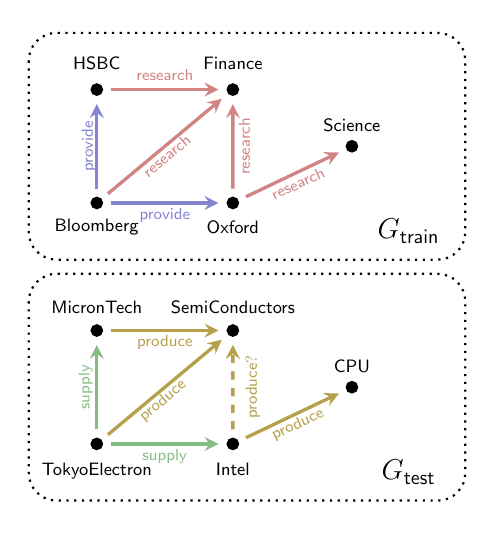
\begin{tikzpicture}[scale=0.9,
        every node/.style={circle, draw, fill=black, inner sep=2pt, line width=0.5pt}, 
        line width=1.2pt, 
        >=stealth,
        shorten >=3pt, 
        shorten <=3pt,
        transform shape
    ]
    \definecolor{cartoonred}{RGB}{190,80,80}
    \definecolor{cartoonblue}{RGB}{80,80,190}
    \definecolor{cartoongreen}{RGB}{80,160,80}
    \definecolor{cartoonyellow}{RGB}{150,120,0}
    \begin{scope}[scale=0.8]
        % Nodes
        \node (pl)[label={[font=\small, xshift = 0em, yshift = -0.5em]90:$\mathsf{HSBC}$}] at (0,0) {};
        \node (ph)[label={[font=\small, xshift= 0em, yshift = -0.75em]90:$\mathsf{Finance}$}] at (2.4,0) {};
        \node (s)[label={[font=\small, xshift = 0em, yshift = 1.5em]-90:$\mathsf{Bloomberg}$}] at (0,-2) {};
        \node (a)[label={[font=\small, xshift= 0em, yshift=0.7em]-90:$\mathsf{Oxford}$}] at (2.4,-2) {};
        \node (m)[label={[font=\small, xshift = 0em, yshift=-1em]90:$\mathsf{Science}$}] at (4.5,-1) {};

    
        \draw[->, color=cartoonblue!70] (s) to node[midway, above, color=cartoonblue!70, draw=none, fill=none, yshift=-2.2em] {\footnotesize $\mathsf{provide}$} (a);
        \draw[->, color=cartoonblue!70] (s) to node[midway, above, color=cartoonblue!70, draw=none, fill=none, xshift=1.2em, rotate=90] {\footnotesize $\mathsf{provide}$} (pl);
        \draw[->, color=cartoonred!70] (s) to node[midway, above, color=cartoonred!70, draw=none, fill=none, yshift=-1.8em, xshift=1.2em, rotate=40] {\footnotesize $\mathsf{research}$} (ph);
        \draw[->, color=cartoonred!70] (pl) to node[midway, above, color=cartoonred!70, draw=none, fill=none, yshift=-1em] {\footnotesize $\mathsf{research}$} (ph);
        \draw[->, color=cartoonred!70] (a) to node[midway, above, color=cartoonred!70, draw=none, fill=none, xshift=2.3em, rotate=90] {\footnotesize $\mathsf{research}$} (ph);
        \draw[->, color=cartoonred!70] (a) to node[midway, above, color=cartoonred!70, draw=none, fill=none, yshift=-2em, xshift=1em, rotate=25] {\footnotesize $\mathsf{research}$} (m);

        \draw[dotted, fill = none, thick, rounded corners=10pt]
            (-1.2, 1) rectangle (6.5, -3);
        \node (label)[draw=none, fill=none] at (5.5, -2.5) {\Large $G_{\textsf{train}}$};
    \end{scope}
    \begin{scope}[yshift=-3.4cm,scale=0.8]
        % Nodes
        \node (pl)[label={[font=\small, xshift = 0em, yshift = -1.7em]90:$\mathsf{Micron Tech}$}] at (0,0) {};
        \node (ph)[label={[font=\small, xshift= 0em, yshift = -2.5em]90:$\mathsf{SemiConductors}$}] at (2.4,0) {};
        \node (s)[label={[font=\small, xshift = 0em, yshift = 2em]-90:$\mathsf{Tokyo Electron}$}] at (0,-2) {};
        \node (a)[label={[font=\small, xshift= 0em, yshift=0.2em]-90:$\mathsf{Intel}$}] at (2.4,-2) {};
        \node (m)[label={[font=\small, xshift = 0em, yshift=-0.5em]90:$\mathsf{CPU}$}] at (4.5,-1) {};
    
        % Hyperedges
         \draw[->, color=cartoongreen!70] (s) to node[midway, above, color=cartoongreen!70, draw=none, fill=none, yshift=-2.1em] {\footnotesize $\mathsf{supply}$} (a);
        \draw[->, color=cartoongreen!70] (s) to node[midway, above, color=cartoongreen!70, draw=none, fill=none, xshift=0.9em, rotate=90] {\footnotesize $\mathsf{supply}$} (pl);
        \draw[->, color=cartoonyellow!70] (s) to node[midway, above, color=cartoonyellow!70, draw=none, fill=none, yshift=-2em, xshift=1em, rotate=40] {\footnotesize $\mathsf{produce}$} (ph);
        \draw[->, color=cartoonyellow!70] (pl) to node[midway, above, color=cartoonyellow!70, draw=none, fill=none, yshift=-2.3em] {\footnotesize $\mathsf{produce}$} (ph);
        \draw[->, dashed, color=cartoonyellow!70] (a) to node[midway, above, color=cartoonyellow!70, draw=none, fill=none, xshift=2.9em, rotate=90] {\footnotesize $\mathsf{produce?}$} (ph);
        \draw[->, color=cartoonyellow!70] (a) to node[midway, above, color=cartoonyellow!70, draw=none, fill=none, yshift=-2em, xshift=1em, rotate=25] {\footnotesize $\mathsf{produce}$} (m);

        
        \draw[dotted, fill = none, thick, rounded corners=10pt]
            (-1.2, 1) rectangle (6.5, -3);
        \node (label)[draw=none, fill=none] at (5.5, -2.5) {\Large $G_{\textsf{test}}$};
    \end{scope}
    \end{tikzpicture}
    \vspace{-1em}
    \caption{
    Training is over relations $\mathsf{provide}$ and $\mathsf{research}$, and testing is over structurally similar relations $\mathsf{supply}$ and $\mathsf{produce}$. }
    \label{fig:relational-hypergraph}
    \vspace{-1em}
\end{figure}

Knowledge Graph Foundation Models (KGFMs) gained significant attention~\citep{galkin2023ultra,mao2024positiongraphfoundationmodels} for their success in link prediction tasks involving \emph{unseen entities and relations} on knowledge graphs (KGs). 
% 
These models aim to generalize across different KGs by effectively learning \emph{relation invariants}: properties of relations that are transferable across KGs of different relational vocabularies~\citep{gao2023double}. 
% 
KGFMs learn representations of relations by relying on their structural roles in the KG, which can be transferred to novel relations based on their ``structurally similarities'' to the observed relations.

%\emph{Which structural properties of relations lead to more expressive KGFMs?}

\begin{example}
Consider the two KGs from \Cref{fig:relational-hypergraph} which use disjoint sets of relations. Suppose that the model is trained on $G_\text{train}$ and the goal is to predict the missing link $\mathsf{produce}(\mathsf{Intel},\mathsf{SemiConductors})$  in $G_\text{test}$.
%
Ideally, the model will predict the link by learning relation invariants that map $\mathsf{produce} \mapsto \mathsf{research}$ and $\mathsf{supply} \mapsto \mathsf{provide}$, as the {\em structural role} of these relations are similar in the respective graphs, even if the relations {\em themselves} differ. \hfill \exend
\end{example}
%This example highlights the importance of learning relation invariants to make accurate predictions over unseen KGs.


The dominant approach~\citep{geng2022relationalmessagepassingfully,ingram,galkin2023ultra} for computing relation invariants is by learning relational embeddings over a \emph{graph of relations}. In this graph, each node represents a relation type from the original KG and each edge represents a connection between two relations. 
 \begin{wrapfigure}{r}{3.1cm}
 \vspace{-1.5em}
     \centering
     % https://q.uiver.app/#q=WzAsMyxbMCwwLCJcXGJ1bGxldCJdLFsxLDAsIlxcYnVsbGV0Il0sWzIsMCwiXFxidWxsZXQiXSxbMCwxLCJcXGFscGhhIl0sWzEsMiwiXFxiZXRhIl1d
 \[\begin{tikzcd}
 	\bullet & \bullet & \bullet
 	\arrow["\alpha", from=1-1, to=1-2]
 	\arrow["\beta", from=1-2, to=1-3]
 \end{tikzcd}\]
 \vspace{-2em}
 \caption{A simple motif of a path of length two.}
     \label{fig:path-of-length-2}
 \end{wrapfigure}
One prominent choice of these connections is to identify whether two relations in the original KG match a set of shared patterns known as \emph{graph motifs}: small, recurring subgraphs that capture essential relational structures within the KG. \Cref{fig:path-of-length-2} depicts a simple motif: a path of length two, connecting three entities via two relations (i.e., a \emph{binary motif}). 
% 
For instance,  the relations $\mathsf{provide}$ and $\mathsf{research}$ are connected via the entity $\mathsf{Oxford}$ in \Cref{fig:relational-hypergraph}, and hence match this motif with the map $\alpha \mapsto \mathsf{provide}$, $\beta \mapsto \mathsf{research}$. %and creating an edge from $\mathsf{provide}$ to $\mathsf{research}$ in the relation graph.}

%For example, a simple motif on KGs could be a path of length two, connecting three entities via two relations, as shown in \Cref{fig:path-of-length-2}.  
%In our running example from \Cref{fig:relational-hypergraph} the entity $\mathsf{Bloomberg}$ $\mathsf{Oxford}$ appears as the \emph{head} of the relation $\mathsf{provide}$ as well as the \emph{tail} of the relation $\mathsf{research}$. 

%One prominent choice of these connections is to identify whether two relations in the original KG match a set of shared patterns known as \emph{graph motifs}: small, recurring subgraphs that capture essential relational structures within the KG.
%For example, a simple motif on KGs could be a path of length two, connecting three entities via two relations, as shown in \Cref{fig:path-of-length-2}. 
% 
%
%One possibility is to build a graph of relations summarizing such relationships, where all the relations from $G_\text{train}$ will appear as nodes in this new graph that are connected to each other using fundamental relations, e.g.,  $\mathsf{provide}$ will be connected to $\mathsf{research}$ with a special relation type \emph{head-to-tail ($h2t$)} indicating their interaction. \hfill \exend

%\begin{figure}[t]
% \vspace{-1.5em}
%\centering
%\begin{tikzpicture}[
%    every node/.style={circle, draw, fill=black, inner sep=1.5pt}, 
%    >=stealth,
%    shorten >=1.5pt, 
%    shorten <=1.5pt,
%    line width=0.8pt
%]
%    % Nodes
%    \node[fill=none,draw=none] (name1) at (-2.5,0) {\emph{h2t}:};
%    \node (A) at (0, 0) {};
%    \node (B) at (1.5, 0) {};
%    \node (C) at (3, 0) {};

%    % Text to the left
%    \node[draw=none, fill=none, anchor=east] at ($(A) - (0.5, 0)$) {\((\alpha, \beta)\)};

%     % Arrows
%    \draw[->] (A) to node[midway, above, draw=none, fill=none] {\(\alpha\)} (B);
%    \draw[->] (B) to node[midway, above, draw=none, fill=none] {\(\beta\)} (C);
    
%    % Nodes
%    \node[fill=none,draw=none] (name2) at (-2.5,-0.8) {\emph{t2h}:};
%    \node (D) at (0, -0.8) {};
%    \node (E) at (1.5, -0.8) {};
%    \node (F) at (3, -0.8) {};

%    % Text to the left
%    \node[draw=none, fill=none, anchor=east] at ($(D) - (0.5, 0)$) {\((\alpha, \beta)\)};
    
%    % Arrows
%    \draw[->] (E) to node[midway, above, draw=none, fill=none] {\(\alpha\)} (D);
%    \draw[->] (F) to node[midway, above, draw=none, fill=none] {\(\beta\)} (E);

%    % Nodes
%    \node[fill=none,draw=none] (name3) at (-2.5,-1.6) {\emph{h2h}:};
%    \node (G) at (0, -1.6) {};
%    \node (H) at (1.5, -1.6) {};
%    \node (I) at (3, -1.6) {};

%    % Text to the left
%    \node[draw=none, fill=none, anchor=east] at ($(G) - (0.5, 0)$) {\((\alpha, \beta)\)};
    
%    % Arrows
%    \draw[->] (G) to node[midway, above, draw=none, fill=none] {\(\alpha\)} (H);
%    \draw[->] (I) to node[midway, above, draw=none, fill=none] {\(\beta\)} (H);

%    % Nodes
%    \node[fill=none,draw=none] (name4) at (-2.5,-2.4) {\emph{t2t}:};
%    \node (J) at (0, -2.4) {};
%    \node (K) at (1.5, -2.4) {};
%    \node (L) at (3, -2.4) {};

%    % Text to the left
%    \node[draw=none, fill=none, anchor=east] at ($(J) - (0.5, 0)$) {\((\alpha, \beta)\)};
    
%    % Arrows
%    \draw[->] (K) to node[midway, above, draw=none, fill=none] {\(\alpha\)} (J);
%    \draw[->] (K) to node[midway, above, draw=none, fill=none] {\(\beta\)} (L);
%\end{tikzpicture}
% \vspace{-2em}
%\caption{The 4 motifs used by $\ultra$ are shown here. %$\textit{h2t}$ represents ``head-to-tail," with the others following similarly. 
%Note that $\textit{h2t}$ and $\textit{t2h}$ are isomorphic but with different relation ordering.
%}
%\label{fig:motifs-in-ULTRA}
%\end{figure}

%The dominant approach~\citep{geng2022relationalmessagepassingfully,ingram,galkin2023ultra} for learning relation invariants is to generate relational embeddings over a \emph{graph of relations}, where each node represents a relation type in the original KG and each edge denotes a relation between two relations. 


%The prominent approach in KGFMs is to learn from such fundamental relations between relation types. For example, ULTRA is a KGFM that uses \emph{head-to-tail (ht)}, \emph{tail-to-head (th)}, \emph{head-to-head (hh)}, and \emph{head-to-tail (tt)} relations as fundamental relation types.

%Technically, each of these fundamental relationships corresponds to identifying whether two relations in the original KG match a set of shared patterns known as \emph{graph motifs}: small, recurring subgraphs that capture essential relational structures within the KG.  The correspondence is depicted in \Cref{fig:motifs-in-ULTRA}: each of these fundamental relations correspond to a simple motif on KGs that is a path of length two, connecting three entities via two relations.


%In this paper, 
We saliently argue that existing models limit themselves to binary motifs, which restricts their ability to capture complex interactions involving more relations. We investigate the expressive power of these models, specifically, how the choice of motifs impacts the model's ability to capture relation invariants and help distinguish between different relational structures. Prior works have extensively studied %the expressive power of 
relational message-passing neural networks on KGs~\citep{barcelo2022wlgorelational,huang2023theory}, but these results do \emph{not} apply to KGFMs, which is the focus of our work.
%primarily focus on node invariants and do \emph{not} extend to KGFMs that capture both node and relation invariants.


\textbf{Approach.} We introduce \underline{MOT}if-\underline{I}nduced \underline{F}ramework for KGFMs~($\mgnn$) based on learning relation invariants from arbitrary (not necessarily binary) graph motifs. $\mgnn$ first constructs a \emph{relational hypergraph}, where each node corresponds to a relation in the original KG, and each \emph{hyperedge} represents a match of relations to a motif in the original KG. Then, it performs message passing over the relational hypergraph to generate relation representations, which are used in message passing over the original KG to enable link prediction over novel relations. Importantly, $\mgnn$ is a general framework that strictly subsumes existing KGFMs such as $\ultra$~\citep{galkin2023ultra} and $\ingram$~\citep{ingram} as detailed in \Cref{sec: motif_captures_KGFMs}, and provides a principled approach for enhancing the expressive power of other KGFMs such as TRIX~\citep{zhang2024trix} and RMPI~\citep{geng2022relationalmessagepassingfully}. 

%Theoretically, 
%we establish 
%a \emph{necessary} 
%conditions under which a newly introduced motif enhances the expressiveness of a KGFM within the framework of $\mgnn$.
%
% 
% We further conduct a thorough expressiveness study via relational Weisfeiler-Leman characterization~\citep{huang2023theory,huang2024link} to investigate which relations and links can be distinguished by $\mgnn$ and $\ultra$.
% \todo{Are we including this?}
% , and further study the logical expressiveness of $\mgnn$ to identify what properties of relations and links can be learned following~\citet{BarceloKM0RS20,huang2023theory}. 

\textbf{Contributions.} Our contributions can be summarized as follows:
\begin{itemize}[leftmargin=.7cm]
    \item We introduce $\mgnn$ as a general framework capable of integrating \emph{arbitrary} graph motifs into KGFMs, subsuming existing KGFMs such as $\ultra$ and $\ingram$.
    \item To the best of our knowledge, we provide the \emph{first} rigorous analysis on the expressive power of KGFMs. Our study explains the capabilities and limitations of existing KGFMs in capturing relational invariants.
%    \item We introduce $\mgnn$ as a unified framework capable of equipping  \emph{arbitrary} graph motifs to compute invariants on both nodes and relations, capturing existing KGFMs such as $\ultra$ and $\ingram$.
    \item We identify a \emph{sufficient} condition under which a newly introduced motif enhances the expressiveness of a KGFM within the framework of $\mgnn$. Using this theoretical recipe, we derive a new KGFM that is provably more expressive than $\ultra$.
   % that ensures a new motif enhances the expressiveness of a KGFM under $\mgnn$, and we derive a new KGFM that is provably more expressive than $\ultra$.
    \item %We conduct extensive empirical analysis over a wide range of real-world KGs and synthetic experiments, validating our theoretical findings. 
    Empirically, we conduct an extensive analysis on $54$ KGs from diverse domains and validate our theoretical results through synthetic and real-world experiments. %We also observe that the performance quickly degrades if we use insufficiently expressive motifs for the task.
\end{itemize}

%All proofs of the technical results can be found in the appendix of the paper along with the additional experiments. 



\section{Related work}

\textbf{Transductive and inductive (on node) link prediction.} Link prediction on KGs has been extensively studied in the literature. Early approaches like TransE~\citep{brodes2013transe}, RotatE~\citep{sun2019rotate}, and BoxE~\citep{abbound2020boxe} focus on the \emph{transductive} setting, 
where learned entity 
%and relation 
embeddings are fixed, and thus 
%where fixed embeddings for each entity and relation are learned, making them inapplicable for unseen 
inapplicable to unseen 
entities at test time. 
%Early 
Multi-relational GNNs such as RGCN~\citep{schlichtkrull2017modeling} and CompGCN~\citep{vashishth2020compositionbased} remain transductive as they store entity and relation embeddings as parameters. To overcome this limitation, \citet{grail2020teru} introduce GraIL, which enables 
\emph{inductive} link prediction via the {\em labeling trick}. 
%employs the {\em labeling trick} \citep{LabelingTrick2021} to enable \emph{inductive} link prediction on nodes. 
%Building on this approach, 
NBFNet \citep{zhu2022neural}, %followed by 
A*Net~\citep{zhu2023anet}, RED-GNN~\citep{zhang2022redgnn}, and AdaProp~\citep{adaprop}, 
provide improvements 
by leveraging conditional message-passing, which is provably more expressive~\citep{huang2023theory}.
%further improved inductive link prediction by leveraging conditional message-passing, which is provably more expressive~\citep{huang2023theory}. 
These models, once trained, can only be applied to KGs with the same relational vocabulary, limiting their applicability
to graphs with unseen relations. %at inference.

\textbf{Inductive (on node and relation) link prediction.}
$\ingram$~\citep{ingram} was one of the first approaches to study inductive link prediction over both new nodes and unseen relations by constructing a weighted relation graph to learn new relation representations. \citet{galkin2023ultra} extended this idea with the $\ultra$ architecture, which constructs a multi-relational graph of fundamental relations and leverages conditional message passing to enhance performance. $\ultra$ was among the first KGFMs to inspire an entire field of research~\citep{mao2024positiongraphfoundationmodels}. Concurrently, RMPI~\citep{geng2022relationalmessagepassingfully} explored generating multi-relational graphs through local subgraph extraction while also incorporating ontological schema. 
%
\citet{gao2023double} introduced the concept of \emph{double-equivariant} GNNs, which establish invariants on nodes and relations by leveraging subgraph GNNs in the proposed ISDEA framework to enforce double equivariance precisely. MTDEA~\citep{zhou2023multitaskperspetivelinkprediction} 
expands this framework %expanded on this idea by incorporating 
with an adaptation procedure for multi-task generalization.
%
Further, TRIX~\citep{zhang2024trix}  expands on $\ultra$ with recursive updates of relation and entity embeddings. 
%Recently, TRIX~\citep{zhang2024trix} was proposed as a more expressive KGFM based on $\ultra$, using recursive updates of relation and entity embeddings. 
Finally, KG-ICL~\citep{cui2024prompt} introduced a new KGFM utilizing in-context learning with a unified tokenizer for entities and relations. 
%
%Despite recent advancements in KGFMs, our understanding of their theoretical capabilities remains limited.

\textbf{Link prediction on relational hypergraphs.} 
Relational hypergraphs 
are a generalization of KGs used to 
represent higher-arity relational data.
%Relational hypergraphs have been introduced to represent higher-arity relational data, serving as a generalization of KGs. 
Work on link prediction in relational hypergraphs first focused on shallow embeddings
~\citep{wen2016representation, liu2020tensor, fatemi2020knowledge}, and later %models such as 
%Several shallow embedding models~\citep{wen2016representation, liu2020tensor, fatemi2020knowledge} have been proposed for the link prediction task using relational hypergraphs. 
%Next, 
G-MPNN~\citep{yadati2020gmpnn} and RD-MPNNs~\citep{zhou2023rdmpnn} %emerged as prominent models that  %specifically designed to 
advanced by  
incorporating message passing.
%incorporate message passing.
Recently, \citet{huang2024link} conducted an in-depth expressivity study on these models and proposed $\hcnets$, extending conditional message-passing to relational hypergraphs and achieving strong results on inductive link prediction.  


\section{Preliminaries}
\textbf{Knowledge graphs.} A \emph{knowledge graph} (KG) is a tuple ${G=(V,E,R)}$, where $V$ is a set of nodes, $R$ is the set of relation types and $E\subseteq  V \times R \times V$ is a set of labeled edges, or {\em facts}. We write $r(u,v)$ to denote a labeled edge, or a fact, where $r\in R$ and $u,v\in V$. 
%For instance, the fact {\em ``Paris is the capital of France''} can be represented as $\mathsf{Capital}(\mathsf{Paris},\mathsf{France})$. 
A (potential) \emph{link} in $G$ is a triple $r(u,v)$ in $V \times R \times V$ that may or may not be a fact in $G$. The \emph{neighborhood} of node $v\in V$ relative to a relation $r \in R$ is $\mathcal{N}_r(v) := \{u \mid r(u,v) \in E\}$.  

\textbf{Relational hypergraphs.} A \emph{relational hypergraph} is a tuple $G = (V,E,R)$, where $V$ is a set of nodes, $R$ is a set of relation types, and $E$ a set of \emph{hyperedges} (or {\em facts}) of the form $e=r(u_1, \ldots, u_k) \in E$ where $r \in R$ is a relation type, $u_1, \ldots, u_k \in V$ are nodes, and $k=\mathtt{ar}(r)$ is the arity of the relation $r$. We write $\rho(e)$ as the relation type $r \in R$ of the hyperedge $e \in E$, and $e(i)$ to refer to the node in the $i$-th arity position of the hyperedge $e$.


\textbf{Homomorphisms.} 
A  (\emph{node-relation}) \emph{homomorphism} from a KG ${G=(V,E,R)}$ to a KG ${G'=(V',E',R')}$ is a pair of mappings $h = (\pi,\phi)$, where 
$\pi: V \to V'$ and $\phi: R \to R'$, such that for every fact  
$r(u,v)$ in $G$, the fact $\phi(r)(\pi(u),\pi(v))$ belongs to $G'$. 
The \emph{image} $h(G)$ of $h$ is the knowledge graph $(\pi(V),h(E),\phi(R))$, where $h(E)$ contains the fact $\phi(r)(\pi(u),\pi(v))$ for each $r(u,v)$ in $G$. 
%Two KGs 
%$G$ and $G'$ are homomorphically equivalent if there are both homomorphisms from $G$ to $G'$ and from $G'$ to $G$. 
% 
  

%Finally, a KG $G$ is a \emph{core} if every homomorphism from $G$ to $G$ is surjective, i.e., $h(G) $. Notice that for a graph $G$, there is a unique (up to isomorphism) graph $H$ that is a both a core and homomorphically equivalent to $G$. This graph $H$ is called the \emph{core} of $G$.

\textbf{Isomorphism, relation invariants, link invariants.} 
An \emph{isomorphism} from KG ${G=(V,E,R)}$ to KG ${G'=(V',E',R')}$ is a pair of bijections $(\pi,\phi)$, where
$\pi: V \to V'$ and $\phi: R \to R'$, such that every fact  
$r(u,v)$ is in $G$ if and only if the fact $\phi(r)(\pi(u),\pi(v))$ is in $G'$.
Two graphs are {\em isomorphic} if there is an isomorphism between them.
%If there is an isomorphism from $G$ to $G'$, we say that these two KGs are {\em isomorphic}. 
For $k\geq 1$, a \emph{$k$-ary relation invariant} is a function $\xi$ associating to each KG $G=(V,E,R)$ a function $\xi(G)$ with domain $R^k$ such that for every isomorphic KGs $G$ and $G'$, every isomorphism $(\pi,\phi)$, and every tuple $\bar{r}\in R^k$ of relations in $G$, we have $\xi(G)(\bar{r})=\xi(G')(\phi(\bar{r}))$. A \emph{link invariant} is a function $\omega$ assigning to each KG $G=(V,E,R)$ a function $\omega(G)$ with domain $V\times R\times V$ such that for every isomorphic KGs $G$ and $G'$, every isomorphism $(\pi,\phi)$, and every link $q(u,v)$ in $G$, we have $\omega(G)(q(u,v))=\omega(G')(\phi(q)(\pi(u),\pi(v)))$.



\section{$\mgnn$: A general framework for KGFMs }
\label{sec: framework}

We present $\mgnn$, as a very general framework for KGFMs.  %$\mgnn$ extends $\ingram$~\citep{ingram} and $\ultra$~\citep{galkin2023ultra} by enabling the use of arbitrary graph motifs, and can be easily adapted to suit other KGFMs~\citep{geng2022relationalmessagepassingfully, zhang2024trix}.
Given a KG $G = (V,E,R)$, $\mgnn$ computes an encoding for each potential link $q(u,v)$ in $G$
%, where $q \in R$ and $u,v \in V$ 
following three steps:

\begin{enumerate}[leftmargin=.5cm]
    \item  \lift: Use a set ${\cal F}$ of motifs to compute a relational hypergraph $\lift_{{\cal F}}(G) = (V_\lift,E_\lift,R_\lift)$, using a procedure called \lift.
    \item \textsc{Relation encoder}: Apply a relation encoder on the hypergraph $\lift_{{\cal F}}(G)$ to obtain relation representations. 
    \item  \textsc{Entity Encoder}:  Use the relation representations from Step 2 and apply an entity encoder on the KG $G$ to obtain final link encodings. %, and use the resulting representations to obtain final link encodings.
\end{enumerate}


The overall process is illustrated in \Cref{fig:mgnn_arch} and we now detail each of the steps.


%First, we use a set ${\cal F}$ of motifs to compute the relational hypergraph $\lift_{{\cal F}}(G) = (V_\lift,E_\lift,R_\lift)$, and apply a relation encoder over this hypergraph. Then, we come back to $G$, encode its relations according to the relation encoding, and use them to obtain final link encodings. The process is illustrated in \Cref{fig:mgnn_arch}.


\begin{figure*}[ht!]
    \centering
    \vspace{-4em}
    \begin{tikzpicture}[
        every node/.style={circle, draw, fill=white, inner sep=2pt, line width=0.5pt}, 
        line width=1.2pt, 
        >=stealth,
        shorten >=3pt, 
        shorten <=3pt,
        transform shape,
        square/.style={regular polygon,regular polygon sides=4},
        triangle/.style={regular polygon,regular polygon sides=3},
    ]
    \definecolor{cartoonred}{RGB}{190,80,80}
    \definecolor{cartoonblue}{RGB}{80,80,190}
    \definecolor{cartoongreen}{RGB}{80,190,80}
    \definecolor{cartoonyellow}{RGB}{190,128,0}
    \definecolor{darkgreen}{RGB}{1, 50, 32}
    \begin{scope}[transform shape, scale=0.88]
        \node (A)[label={[font=\large]135:$u$}]  at (0.0, 0.0) {}; 
        \node (B) at (1.152, 0.64) {}; 
        \node (D) at (0.96, -0.64) {}; 
        \node (E) at (2.112, -0.768) {}; 
        \node (F)[label={[font=\large]45:$v$}] at (2.88, 0.192) {};  
    
        
        % Arrows with specified colors and bend
        \draw[->, bend left=15] (A) to node[midway, above, draw=none, fill=none] {$r_2$} (B);
        \draw[->, bend right=15] (B) to node[midway, right, draw=none, fill=none] {$r_3$} (D);
        \draw[->, bend right=5] (D) to node[midway, above, draw=none, fill=none] {$r_1$} (E);
        
        \draw[->,  bend left=15] (E) to node[midway, left, draw=none, fill=none] {$r_3$} (F);
        \draw[->, bend right=15] (F) to node[midway, above, draw=none, fill=none] {$r_4$} (B);

        % % The query arrow
        \draw[->, dashed,  bend right=90, looseness=1.5] (A) to node[midway, below, draw=none, fill=none] {$r_1?$} (F);

        \node[draw=none, fill=none,inner sep=10pt,label={[yshift=0.1cm]center: Knowledge Graph $G$}] () at (1.5,1.7) {};

        % Vertical dotted line
    \draw[dotted] (4,-2) -- (4,2); 

    \end{scope}
    \begin{scope}[transform shape, scale=0.80, xshift = 7.5cm, yshift = 0cm,line width=0.6pt,inner sep=0pt, shorten >=-0.5pt, 
        shorten <=-0.5pt]
        \node[draw=none, fill=none] (n0)  at (-1.8, 0) {$P_1:$};
        \node[draw=none] (n1)  at (-0.8, 0) {$\bullet$}; 
        \node[draw=none]  (n2) at (0.2, 0) {$\bullet$}; 
        \node[draw=none]  (n3) at (1.2, 0) {$\bullet$}; 

        \node[draw=none, fill=none]  (p0)  at (-1.8, -0.5) {$P_2:$}; 
        \node[draw=none]  (p1)  at (-1.3, -0.5) {$\bullet$}; 
        \node[draw=none]  (p2) at (-0.2, -0.5) {$\bullet$}; 
        \node[draw=none]  (p3) at (0.7, -0.5) {$\bullet$};
        \node[draw=none]  (p4) at (1.7, -0.5) {$\bullet$};
       
        
        \draw[->] (n1) to node[midway, above, draw=none, fill=none] {$\alpha$}(n2);
        \draw[->] (n2) to node[midway, above, draw=none, fill=none] {$\beta$}(n3);

        \draw[->] (p1) to node[midway, below, draw=none, fill=none] {$\alpha$}(p2);
        \draw[->] (p2) to node[midway, below, draw=none, fill=none] {$\beta$}(p3);
        \draw[->] (p3) to node[midway, below, draw=none, fill=none] {$\gamma$}(p4);


        


        \draw[dotted, fill = none, thick, rounded corners=10pt]
            (-2.4, 0.5) rectangle (2, -1);
        % \node (label)[draw=none, fill=none] at (1, -1.2) {Motif set ${\cal F}$};

        % \node (label)[draw=none, fill=none] at (-2.7, -0.25) { ${\cal F}$};

        \node (caption)[scale=1.15,draw=none, fill=none] at (-0.3, 2) {1. $\lift$ $G$ with motif set $\gF$};
        

    \end{scope}
    \begin{scope}[transform shape, scale=0.88, xshift = 11cm, yshift = -0.3cm,line width=0.6pt]
        \node (B)[square,color = cartoonblue, label={[font=\large]45:$r_1$}]  at (0, 1) {}; 
        \node (R)[square,color = cartoonred,label={[font=\large]135:$r_2$}]  at (-1, 0) {}; 
        \node (G)[square,color = cartoongreen,label={[font=\large]45:$r_3$}]  at (1, 0) {}; 
        \node (Y)[square,color = cartoonyellow,label={[font=\large]-135:$r_4$}]  at (0, -1) {}; 
        
        \draw[->] (R) to node[midway, above, draw=none, fill=none,yshift=-0.3em] {\scriptsize $P_1$}(G);
        \draw[<->] (B) to node[midway, above, draw=none, fill=none,yshift=-0.3em,xshift=0.3em] {\scriptsize $P_1$} (G);
        \draw[<->] (Y) to node[midway, right, draw=none, fill=none,yshift=-0.3em] {\scriptsize $P_1$} (G);
        % \draw[->] (R) to (Y);
        
        
        \draw[draw = none, fill = gray, fill opacity=0.2, thick, rounded corners=10pt] 
            ($(B)+(-0.1,0.3)$) -- 
            ($(Y)+(-0.1,-0.3)$) -- 
            ($(G)+(0.3,0)$) -- cycle;

        \draw[draw = none, fill = gray, fill opacity=0.2, thick, rounded corners=10pt] 
            ($(B)+(0,0.3)$) -- 
            ($(R)+(-0.3,-0.1)$) -- 
            ($(G)+(0.3,-0.1)$) -- cycle;

        \node[draw=none, fill=none] (n0)  at (-0.8, 0.7) {\scriptsize \textcolor{gray}{$P_2$}};
        \node[draw=none, fill=none] (n1)  at (-0.3, -0.5) {\scriptsize \textcolor{gray}{$P_2$}};
        
        % \node[draw=none, fill=none,inner sep=10pt,label={[yshift=0.1cm]center: 2. \textsc{Relation Encoder} over $\lift_{\cal F}(G)$}] () at (0,2) {};
        \node[draw=none, fill=none, inner sep=10pt, align=center] 
    at (0,2) 
    {2. \textsc{Relation Encoder} \\ over $\lift_{\cal F}(G)$};

    \end{scope}
    \begin{scope}[transform shape, scale=0.88, xshift = 14cm]
        \node (A)[label={[font=\large]135:$u$},fill=cartoonblue]  at (0.0, 0.0) {};
        \node[fill=yellow] (B) at (1.152, 0.64) {}; 
     
        \node[fill=yellow] (D) at (0.96, -0.64) {}; 
        \node[fill=yellow] (E) at (2.112, -0.768) {}; 
        \node[fill=yellow,double] (F)[label={[font=\large]45:$v$}] at (2.88, 0.192) {};  
  
        
        % Arrows with specified colors and bend
        \draw[->, color=cartoonred, bend left=15] (A) to  (B);

        \draw[->, color=cartoongreen, bend right=15] (B) to (D);
        \draw[->, color=cartoonblue, bend right=5] (D) to  (E);
        
        \draw[->, color=cartoongreen, bend left=15] (E) to  (F);

        \draw[->, color=cartoonyellow, bend right=15] (F) to (B);
       
        \node[draw=none, fill=none, inner sep=10pt, align=center] 
    at (1.5,1.7) 
    {3. \textsc{Entity Encoder} \\ over $G$};


        
        % % The query arrow
        \draw[->, dashed,color=cartoonblue,  bend right=90, looseness=1.5] (A) to node[midway, below, draw=none, fill=none] {$r_1?$} (F);
    \end{scope}

    \node[draw=none,fill=none,inner sep=10pt](G1) at (2.5,0.5){};
    \node[draw=none,fill=none,inner sep=10pt](G21) at (8.8,0.5){};

    \draw[->, black, bend left=10] (G1) to (G21);
   

    % \node[draw=none,fill=none,inner sep=10pt](G22) at (10,-1.5){};
    % \node[draw=none,fill=none,inner sep=10pt](G3) at (13,-1.5){};

    % \draw[->, dashed, bend right=15] (G22) to node[midway, below, draw=none, fill=none,yshift=1.2cm] {Assign $\vh_{r|r_1}$ for all $r \in R$} (G3);

    
    
    \end{tikzpicture}
    \vspace{-1em}
    \caption{Overall framework of $\mgnn({\cal F})$ over the motif set ${\cal F}$: Given a query $r_1(u,v)$, $\mgnn({\cal F})$ first applies the $\lift_{{\cal F}}$ operation to generate the relational hypergraph $(V_\lift,E_\lift,R_\lift)$ over the set of motifs ${\cal F}$. Then a relation encoder is applied to generate a relation representation (indicated by color) conditioned on query $r_1$, followed by an entity encoder that conducts conditional message passing. }
    \label{fig:mgnn_arch}
\end{figure*}

% \begin{figure*}[ht!]
%     \centering
%     \vspace{-4em}
%     \begin{tikzpicture}[
%         every node/.style={circle, draw, fill=white, inner sep=2pt, line width=0.5pt}, 
%         line width=1.2pt, 
%         >=stealth,
%         shorten >=3pt, 
%         shorten <=3pt,
%         transform shape,
%         square/.style={regular polygon,regular polygon sides=4},
%         triangle/.style={regular polygon,regular polygon sides=3},
%     ]
%     \definecolor{cartoonred}{RGB}{190,80,80}
%     \definecolor{cartoonblue}{RGB}{80,80,190}
%     \definecolor{cartoongreen}{RGB}{80,190,80}
%     \definecolor{cartoonyellow}{RGB}{190,128,0}
%     \definecolor{darkgreen}{RGB}{1, 50, 32}
%     \begin{scope}[transform shape, scale=0.88]
%         \node (A)[label={[font=\large]135:$u$}]  at (0.0, 0.0) {}; 
%         \node (B) at (1.152, 0.64) {}; 
%         \node (D) at (0.96, -0.64) {}; 
%         \node (E) at (2.112, -0.768) {}; 
%         \node (F)[label={[font=\large]45:$v$}] at (2.88, 0.192) {};  
    
        
%         % Arrows with specified colors and bend
%         \draw[->, bend left=15] (A) to node[midway, above, draw=none, fill=none] {$r_2$} (B);
%         \draw[->, bend right=15] (B) to node[midway, right, draw=none, fill=none] {$r_3$} (D);
%         \draw[->, bend right=5] (D) to node[midway, above, draw=none, fill=none] {$r_1$} (E);
        
%         \draw[->,  bend left=15] (E) to node[midway, left, draw=none, fill=none] {$r_3$} (F);
%         \draw[->, bend right=15] (F) to node[midway, above, draw=none, fill=none] {$r_4$} (B);

%         % % The query arrow
%         \draw[->, dashed,  bend right=90, looseness=1.5] (A) to node[midway, below, draw=none, fill=none] {$r_1?$} (F);

%         \node[draw=none, fill=none,inner sep=10pt,label={[yshift=0.1cm]center: Knowledge Graph $G$}] () at (1.5,-2.2) {};

%     \end{scope}
%     \begin{scope}[transform shape, scale=0.80, xshift = 6.5cm, yshift = 0cm,line width=0.6pt,inner sep=0pt, shorten >=-0.5pt, 
%         shorten <=-0.5pt]
%         \node[draw=none, fill=none] (n0)  at (-2, 0) {$P_1:$};
%         \node[draw=none] (n1)  at (-1, 0) {$\bullet$}; 
%         \node[draw=none]  (n2) at (0, 0) {$\bullet$}; 
%         \node[draw=none]  (n3) at (1, 0) {$\bullet$}; 

%         \node[draw=none, fill=none]  (p0)  at (-2, -0.5) {$P_2:$}; 
%         \node[draw=none]  (p1)  at (-1.5, -0.5) {$\bullet$}; 
%         \node[draw=none]  (p2) at (-0.5, -0.5) {$\bullet$}; 
%         \node[draw=none]  (p3) at (0.5, -0.5) {$\bullet$};
%         \node[draw=none]  (p4) at (1.5, -0.5) {$\bullet$};
       
        
%         \draw[->] (n1) to node[midway, above, draw=none, fill=none] {$\alpha$}(n2);
%         \draw[->] (n2) to node[midway, above, draw=none, fill=none] {$\beta$}(n3);

%         \draw[->] (p1) to node[midway, below, draw=none, fill=none] {$\alpha$}(p2);
%         \draw[->] (p2) to node[midway, below, draw=none, fill=none] {$\beta$}(p3);
%         \draw[->] (p3) to node[midway, below, draw=none, fill=none] {$\gamma$}(p4);


        
%         % \draw[draw = none, fill = gray, fill opacity=0.2, thick, rounded corners=10pt] 
%         %     ($(B)+(0,0.3)$) -- 
%         %     ($(R)+(-0.3,-0.1)$) -- 
%         %     ($(G)+(0.3,-0.1)$) -- cycle;

%         \draw[dotted, fill = none, thick, rounded corners=10pt]
%             (-2.4, 0.7) rectangle (2, -1.5);
%         \node (label)[draw=none, fill=none] at (1, -1.2) {Motif set ${\cal F}$};
    

%     \end{scope}
%     \begin{scope}[transform shape, scale=0.88, xshift = 10cm, yshift = -0.3cm,line width=0.6pt]
%         \node (B)[square,color = cartoonblue, label={[font=\large]45:$r_1$}]  at (0, 1) {}; 
%         \node (R)[square,color = cartoonred,label={[font=\large]135:$r_2$}]  at (-1, 0) {}; 
%         \node (G)[square,color = cartoongreen,label={[font=\large]45:$r_3$}]  at (1, 0) {}; 
%         \node (Y)[square,color = cartoonyellow,label={[font=\large]-135:$r_4$}]  at (0, -1) {}; 
        
%         % \draw[->] (B) to (R);
%         % \draw[->] (R) to (B);
%         % \draw[->] (G) to (B);
%         % \draw[->] (Y) to (G);
%         % \draw[->] (G) to (Y);
%         % \draw[->] (R) to (Y);
%         % \draw[->] (G) to (R);
%         \draw[->] (R) to node[midway, above, draw=none, fill=none,yshift=-0.3em] {\scriptsize $P_1$}(G);
%         \draw[<->] (B) to node[midway, above, draw=none, fill=none,yshift=-0.3em,xshift=0.3em] {\scriptsize $P_1$} (G);
%         \draw[<->] (Y) to node[midway, right, draw=none, fill=none,yshift=-0.3em] {\scriptsize $P_1$} (G);
%         % \draw[->] (R) to (Y);
        
        
%         \draw[draw = none, fill = gray, fill opacity=0.2, thick, rounded corners=10pt] 
%             ($(B)+(-0.1,0.3)$) -- 
%             ($(Y)+(-0.1,-0.3)$) -- 
%             ($(G)+(0.3,0)$) -- cycle;

%         \draw[draw = none, fill = gray, fill opacity=0.2, thick, rounded corners=10pt] 
%             ($(B)+(0,0.3)$) -- 
%             ($(R)+(-0.3,-0.1)$) -- 
%             ($(G)+(0.3,-0.1)$) -- cycle;

%         \node[draw=none, fill=none] (n0)  at (-0.8, 0.7) {\scriptsize \textcolor{gray}{$P_2$}};
%         \node[draw=none, fill=none] (n1)  at (-0.3, -0.5) {\scriptsize \textcolor{gray}{$P_2$}};
        
%         \node[draw=none, fill=none,inner sep=10pt,label={[yshift=0.1cm]center: \textsc{Relation Encoder} over $\lift_{\cal F}(G)$}] () at (0,-1.9) {};

%     \end{scope}
%     \begin{scope}[transform shape, scale=0.88, xshift = 13cm]
%         \node (A)[label={[font=\large]135:$u$},fill=cartoonblue]  at (0.0, 0.0) {};
%         \node[fill=yellow] (B) at (1.152, 0.64) {}; 
     
%         \node[fill=yellow] (D) at (0.96, -0.64) {}; 
%         \node[fill=yellow] (E) at (2.112, -0.768) {}; 
%         \node[fill=yellow,double] (F)[label={[font=\large]45:$v$}] at (2.88, 0.192) {};  
  
        
%         % Arrows with specified colors and bend
%         \draw[->, color=cartoonred, bend left=15] (A) to  (B);

%         \draw[->, color=cartoongreen, bend right=15] (B) to (D);
%         \draw[->, color=cartoonblue, bend right=5] (D) to  (E);
        
%         \draw[->, color=cartoongreen, bend left=15] (E) to  (F);

%         \draw[->, color=cartoonyellow, bend right=15] (F) to (B);
       
%         \node[draw=none, fill=none,inner sep=10pt,label={[yshift=0.1cm]center: \textsc{Entity Encoder} over $G$}] () at (1.5,-2.2) {};

        
%         % % The query arrow
%         \draw[->, dashed,color=cartoonblue,  bend right=90, looseness=1.5] (A) to node[midway, below, draw=none, fill=none] {$r_1?$} (F);
%     \end{scope}

%     \node[draw=none,fill=none,inner sep=10pt](G1) at (2,0.8){};
%     \node[draw=none,fill=none,inner sep=10pt](G21) at (8,0.8){};

%     \draw[->, dashed, bend left=15] (G1) to node[midway, above, draw=none, fill=none,yshift=-0.1cm] {$\lift_\gF$} (G21);

%     \node[draw=none,fill=none,inner sep=10pt](G22) at (9,0.8){};
%     \node[draw=none,fill=none,inner sep=10pt](G3) at (12,0.8){};

%     \draw[->, dashed, bend left=15] (G22) to node[midway, above, draw=none, fill=none,yshift=-1.2cm] {Assign $\vh_{r|r_1}$ for all $r \in R$} (G3);

    
    
%     \end{tikzpicture}
%     \vspace{-6em}
%     \caption{Overall framework of $\mgnn({\cal F})$ over the motif set ${\cal F}$: Given a query $r_1(u,v)$, $\mgnn({\cal F})$ first applies the $\lift_{{\cal F}}$ operation to generate the relational hypergraph $(V_\lift,E_\lift,R_\lift)$ over the set of motifs ${\cal F}$. Then a relation encoder is applied to generate a relation representation conditioned on query $r_1$, followed by an entity encoder that conducts conditional message passing with $\vh_{r|r_1}$.}
%     \label{fig:mgnn_arch}
% \end{figure*}


\subsection{\lift}

\newcommand{\eval}{\text{Eval}}

%Motifs are the most common way to obtain information from graphs~\citep{milo2002motif, Menczer_Fortunato_Davis_2020, mao2024positiongraphfoundationmodels}, and MOTIF use them to construct relational hypergraphs. 
%\todo{Xingyue: I modified this as initially it is written "$P = (G,\bar r)$, where $G_M = (V,E,R)$. Could someone check this?"}
%%Juan: checked thanks!
A graph \emph{motif} is a pair $P = (G_M,\bar r)$, where $G_M = (V_M,E_M,R_M)$ is a connected KG and $\bar r$ is a tuple defining an order on the relation set $R_M$. 
%For $P$ a motif, $\rvar(P)$ are the variables in $P$ corresponding to relations (in the second component of triples), $\nvar(P)$ those to nodes (in the first component), and $\var(P)$ all variables.
%
The information extracted by motifs is defined via homomorphisms. 

\begin{definition} 
Let $G$ be a KG and $P = (G_M,\bar r)$ be a motif with $\bar r = (r_1,\dots,r_n)$. 
The \emph{evaluation} $\eval(P,G)$ of $P$ over $G$ is the set of tuples 
$(\phi(r_1),\dots,\phi(r_n))$, for each homomorphism $h = (\pi,\phi)$ from $G_M$ to $G$. \qed 
\end{definition} 

%%%not yet. 
%Further, we say that $h$ is \emph{relation preserving} if 
%%%% maybe all we need is that the arity $h_r(R) = R$. 


%Let ${\cal F} = \{P_1,\dots,P_n\}$ be a set of  motifs. We can use ${\cal F}$ on a KG $G$ to define a relational hypergraph with relation types $P_1,\dots,P_n$. We do this via the \lift\ operation, defined next.

\textbf{The $\lift$ operation.} Given a KG, $\lift$ outputs a relational hypergraph induced by a set of motifs. Let ${\cal F}$ be a set of motifs, and $G = (V,E,R)$ a KG. Then $\lift_{{\cal F}}(G)$ is the relational hypergraph $(V_\lift,E_\lift,R_\lift)$, where $V_\lift=R$, $R_\lift={\cal F}$, and $E_\lift$ is constructed as follows: for each motif $P\in {\cal F}$, and for each tuple $(r_1,\dots,r_n)$ in the evaluation $\eval(P,G)$ of $P$ over $G$,  $P(r_1,\dots,r_n) \in E_\lift$. 

%Let ${\cal F}$ be a set of motifs, and $G = (V,E,R)$ a KG. Then $\lift_{{\cal F}}(G)$ is the relational hypergraph $(V_\lift,E_\lift,R_\lift)$ constructed in the following way. The set of nodes $V_\lift$ correspond to the set $R$ of relations of the original KG $G$. The set $R_\lift$ of relation types correspond to the motifs in ${\cal F}$. Lastly, for each motif $P\in {\cal F}$, and for each tuple $(r_1,\dots,r_n)$ in the evaluation $\eval(P,G)$ of $P$ over $G$, we have $P(r_1,\dots,r_n) \in E_\lift$.


\newcommand{\MR}{\text{MR}}
\subsection{Relation encoder}


%\noindent
%\textbf{Relation encoder.} 
A {\em relation encoder} is a tuple $(\gF, \enc_\lift)$, where $\gF$ is a set of motifs and $\enc_\lift$ computes relation representations for the set $R = V_\lift$ of nodes of $\lift_\gF(G) = (V_\lift,E_\lift,R_\lift)$. Given that our aim is to encode links of the form $q(u,v)$, the encoding computed by $\enc_\lift$ for relation $r \in R$ is \emph{conditioned} on the relation $q\in R$. These encodings are determined by a sequence of features $\vh^{(t)}_{r|q} \in \mathbb{R}^{d(t)}$, for $0\leq t\leq T$, defined iteratively as follows: 
% \todo{do we want to lift the `conditioned` condition?}
\begin{align*}
    \vh_{r|q}^{(0)} = \init_1(q,r), \quad
    \vh_{r|q}^{(t+1)}  =\update_1 \big( \vh_{r|q}^{(t)},  \aggregate_1(M) \big),
\end{align*}
where $\init_1$, $\update_1$, $\aggregate_1$ are differentiable \emph{initialization}, \emph{update}, and \emph{aggregation} functions, respectively, and: 
\begin{multline*} 
M = \llbrace \mes_{\rho(e)} \big(\{(\vh_{r'|q}^{(t)}, j ) \mid \\ 
(r',j) \in \gN^i(e) \} \big) \mid (e,i) \in E_{\lift}(r) \rrbrace. 
\end{multline*} 
In this setting, $\mes_{\rho(e)}$ is a motif-specific \emph{message} function and 
we further define 
$E_{\lift}(r) = 
    \left\{
    (e,i) \mid  e(i)=r, e \in E_\lift, 1 \leq i \leq \mathtt{ar}(\rho(e))
    \right\}$ 
    as the set of edge-position pairs of a node $r$, and $\gN^{i}{(e)}$ as the \emph{positional neighborhood} of a hyperedge $e$ with respect to a position $i$: $\gN^{i}(e)=
    \left\{
    (e(j),j) \mid  j \neq i,  1 \leq j \leq \mathtt{ar}(\rho(e))
    \right\}$. 

We use $\enc_{\lift,q}[r]$ to denote the final relation encoding of a relation $r$ in $G$ when conditioned on $q$, that is, the last layer vector $\vh_{r|q}^{(T)}\in \mathbb{R}^{d(T)}$.  

\textbf{Remark 1}. Observe that the relation encoder computes binary relation invariants provided $\init_1$ is an invariant.  
% \todo{fill the remark 1}



\subsection{Entity encoder}
$\mgnn$ uses an entity encoder to compute a link-level representation of a KG, regardless of its relation vocabulary. 
This works as follows. $\mgnn$ is defined as a tuple $(\enc_{{\rm KG}},(\gF,\enc_\lift))$, where $(\gF,\enc_\lift)$ is a relation encoder and $\enc_{{\rm KG}}$ is an entity encoder that computes node representations over KGs of the form 
$G = (V,E,R)$, 
conditioned on a node $u \in V$ and the relation $q$, according to the following iterative scheme:
%
%For a KG $G = (V,E,R)$ and a query of the form $q(u,?)$ where $u \in V$ and $q \in R$,  
\begin{align*}
\vh_{v|u,q}^{(0)} = \init_2(u,v,q), \quad
\vh_{v|u,q}^{(\ell+1)} = \update_2\big(\vh_{v|u,q}^{(\ell)}, \aggregate_2(N)\big), 
\end{align*} where $\init_2$, $\update_2$, $\aggregate_2$, and $\mes$ are differentiable \emph{initialization}, \emph{update}, \emph{aggregation} and \emph{message} functions, respectively, 
%Here we define $\mathcal{N}_r(v)$ as the \emph{neighborhood} of a node $v\in V$ relative to a relation $r \in R$: $\mathcal{N}_r(v) := \{u \mid r(u,v) \in E\}$.
$v$ is an arbitrary node in $V$, and:
$$
N = \{\!\! \{ \mes(\vh_{w|u,q}^{(\ell)},\enc_{\lift,q}[r])  \mid w \in \mathcal{N}_r(v), r \in R \}\!\!\}.
$$

We use $\enc_{{\rm KG},u,q}[v]$ to denote the encoding of $v$, conditioned on  relation $q$ and source node $u$, which corresponds to $\vh_{v|u,q}^{(L)}\in \mathbb{R}^{d(L)}$ ($L$ being the number of layers).  
Finally, a unary decoder $\dec:\sR^{d(L)} \mapsto [0,1]$ is applied on $\enc_{{\rm KG},q,u}[v]$ to obtain the probability score for the existence of the potential link $q(u,v)$.% for all $v\in V$. 


\textbf{Remark 2}. Observe that the entity encoder computes link invariants provided $\init_2$ is an invariant. 

\section{KGFMs captured by $\mgnn$}
\label{sec: motif_captures_KGFMs}

We revisit the $\ultra$ architecture~\citep{galkin2023ultra} (See details in \Cref{app:ULTRA_def}). The four fundamental relations used in $\ultra$ can be interpreted as the graph motifs illustrated in Figure \ref{fig:motifs-in-ULTRA}. Hence, any $\ultra$ architecture can be represented as a $\mgnn$ architecture, with $\enc_\lift$ and $\enc_\text{KG}$ being specific variants of NBFNets~\citep{zhu2022neural}. 
% It is worth noting that the $\mgnn$ architecture allows for more expressive models, even when using the same motifs as those shown in \Cref{fig:motifs-in-ULTRA}, such as models that can natively handle inverses.
\begin{figure}[t]
% \vspace{-1.5em}
\centering
\begin{tikzpicture}[
    every node/.style={circle, draw, fill=black, inner sep=1.5pt}, 
    >=stealth,
    shorten >=1.5pt, 
    shorten <=1.5pt,
    line width=0.8pt
]
    % Nodes
    \node[fill=none,draw=none] (name1) at (-2.5,0) {\emph{h2t}:};
    \node (A) at (0, 0) {};
    \node (B) at (1.5, 0) {};
    \node (C) at (3, 0) {};

    % Text to the left
    \node[draw=none, fill=none, anchor=east] at ($(A) - (0.5, 0)$) {\((\alpha, \beta)\)};

     % Arrows
    \draw[->] (A) to node[midway, above, draw=none, fill=none] {\(\alpha\)} (B);
    \draw[->] (B) to node[midway, above, draw=none, fill=none] {\(\beta\)} (C);
    
    % Nodes
    \node[fill=none,draw=none] (name2) at (-2.5,-0.8) {\emph{t2h}:};
    \node (D) at (0, -0.8) {};
    \node (E) at (1.5, -0.8) {};
    \node (F) at (3, -0.8) {};

    % Text to the left
    \node[draw=none, fill=none, anchor=east] at ($(D) - (0.5, 0)$) {\((\alpha, \beta)\)};
    
    % Arrows
    \draw[->] (E) to node[midway, above, draw=none, fill=none] {\(\alpha\)} (D);
    \draw[->] (F) to node[midway, above, draw=none, fill=none] {\(\beta\)} (E);

    % Nodes
    \node[fill=none,draw=none] (name3) at (-2.5,-1.6) {\emph{t2t}:};
    \node (G) at (0, -1.6) {};
    \node (H) at (1.5, -1.6) {};
    \node (I) at (3, -1.6) {};

    % Text to the left
    \node[draw=none, fill=none, anchor=east] at ($(G) - (0.5, 0)$) {\((\alpha, \beta)\)};
    
    % Arrows
    \draw[->] (G) to node[midway, above, draw=none, fill=none] {\(\alpha\)} (H);
    \draw[->] (I) to node[midway, above, draw=none, fill=none] {\(\beta\)} (H);

    % Nodes
    \node[fill=none,draw=none] (name4) at (-2.5,-2.4) {\emph{h2h}:};
    \node (J) at (0, -2.4) {};
    \node (K) at (1.5, -2.4) {};
    \node (L) at (3, -2.4) {};

    % Text to the left
    \node[draw=none, fill=none, anchor=east] at ($(J) - (0.5, 0)$) {\((\alpha, \beta)\)};
    
    % Arrows
    \draw[->] (K) to node[midway, above, draw=none, fill=none] {\(\alpha\)} (J);
    \draw[->] (K) to node[midway, above, draw=none, fill=none] {\(\beta\)} (L);
\end{tikzpicture}
 \vspace{-1em}
\caption{The 4 motifs used by $\ultra$ are shown here. $\textit{h2t}$ represents ``head-to-tail", with the others following similarly. 
Note that $\textit{h2t}$ and $\textit{t2h}$ are isomorphic but with different relation ordering.
}
\label{fig:motifs-in-ULTRA}
\end{figure}

$\mgnn$ can also represent a slight variant of the $\ingram$ architecture~\citep{ingram} when we replace the constructed weighted relation graph with a KG. Here the construction of $\lift$ uses a graph motif set $\gF = \{h2h, t2t\}$, with $\enc_\lift$ and $\enc_\text{KG}$ being variants of GATv2~\citep{brody2022attentivegraphattentionnetworks}. Note that the definition of $\mgnn$ allows for unconditional message passing~\citep{huang2023theory} when both $\init_1$ and $\init_2$ are agnostic to the query $q$. %Additionally, a binary decoder is required to compute the probability score.

We also note that, while other KGFMs like RMPI~\citep{geng2022relationalmessagepassingfully} and TRIX~\citep{zhang2024trix} do not technically fall under the framework of $\mgnn$, these models do rely on a $\lift$ operation to construct a graph of relations based on a predefined set of motifs, 
%similarly rely on the $\lift$ operation. This operation constructs a graph of relations based on a predefined set of motifs, 
followed by relation and entity encoders. 
%, $\enc_\lift$ and $\enc_{\text{KG}}$. 
In particular, RMPI constructs an alternative relation graph inspired by the line graph, incorporating the motifs used in $\ultra$ along with two additional motifs, $\textsf{PARA}$ and $\textsf{LOOP}$. In turn, TRIX considers the same set of motifs as $\ultra$ but employs alternating updates on entity and relation representations. %While our expressiveness study of $\mgnn$ is not directly applicable to these methods, it remains fundamental for understanding their properties.


% \todo{Xingyue: made my attempt. Can someone check if this is satisfying?
% Juan: Looks great!!}

% MOTIF can also capture the $\ingram$ architecture \cite{ingram}. ++++ see what to do here ++++
% \todo{(Xingyue: we can say something like, MOTIF can capture a slight "variant" of $\ingram$ architecture where the graph of relation is not a weighted graph but a discrete typed graph? by adopting an unconditional entity and relation encoder. [but the discrete typed graph needs more clarification, and we can push to appendix. We don't want to get too involved since this is a discussion about homomorphism count v.s. homomorphism existence])}

\section{Expressive power}
\label{sec: expressive_power}

%These encodings are invariant under KG isomorphism. Here, an \emph{isomorphism} from KG ${G=(V,E,R)}$ to KG ${G'=(V',E',R')}$ is a pair of bijections $(\pi,\phi)$, where
%$\pi : V \to V'$ and $\phi : R \to R'$, such that every fact $r(u,v)$ is in $G$ if and only if the fact $\phi(r)(\pi(u),\pi(v))$ is in $G'$. If $G = (V,E,R)$ and $G' = (V',E',R')$ are two isomorphic KGs, and $(f_V,f_R)$ is an  isomorphism between $G$ and $G'$, then any $\mgnn$ computes the same encoding for the fact $r(u,v)$ in $G$ and the fact
%$\gF_R(r)(f_V(u),f_V(v))$ in $G'$. 

% \todo{miguel: reference appendix F to the correspondence btw ULTRA and MOTIF. Xingyue: I will rewrite and add a theorem for it.}
$\mgnn$ computes encodings for links in KGs. In this section, we aim to understand which links $\mgnn$ can separate and whether equipping $\mgnn$ with more graph motifs increases its separation power. Hence, our focus is on the potential power obtained when using a particular set ${\cal F}$ of motifs. To that extent, we define $\mgnn({\cal F})$ as the set of all $\mgnn$ instances that use a relation encoder built over ${\cal F}$, that is, the set of all $\mgnn$ instances of the form $(\enc_{\text{KG}},({\cal F},\enc_\lift))$. 

\newcommand{\sep}{\mathsf{sep}}
\newcommand{\conto}{\rightarrow^{co}}
\newcommand{\Conto}{\Rightarrow^{co}}
\newcommand{\F}{\mathcal{F}}

\begin{definition} 
\label{def-refines}
Let $\F$ and $\F'$ be sets of graph motifs.  
Then $\F$ \emph{refines} $\F'$, denoted $\F \preceq \F'$, if for every KG $G$ and potential links $q(u,v)$, $q'(u',v')$ over $G$, whenever every $\mgnn$ instance in $\mgnn(\F)$ encodes $q(u,v)$ and $q'(u',v')$ in the same way, then every $\mgnn$ instance in $\mgnn(\F')$ also encodes $q(u,v)$ and $q'(u',v')$ in the same way. Furthermore, $\F$ and $\F'$ are said to have the same {\em separation power} if both $\F \preceq \F'$ and $\F' \preceq \F$ hold. We denote this as $\F \sim \F'$.
\qed
\end{definition}

Definition \ref{def-refines} captures the idea of the potential to separate, or distinguish, pairs of links in a KG using different sets of graph motifs. Specifically, whenever $\F \preceq \F'$, we know that using $\F'$ will not result in architectures that can separate links that cannot be separated by any $\mgnn$ instance in $\mgnn(\F)$. On the other hand, if $\F \sim \F'$, then we know that $\F$ and $\F'$ can be used interchangeably without altering the potential for separating links in our architectures. 

We start by observing a simple fact: isomorphic graph motifs do not make a difference in terms of 
separation power. %An \emph{isomorphism} from KG ${G=(V,E,R)}$ to KG ${G'=(V',E',R')}$ is a pair of bijections $(\pi,\phi)$, where
%$\pi: V \to V'$ and $\phi: R \to R'$, such that every fact  
%$r(u,v)$ is in $G$ if and only if the fact $\phi(r)(\pi(u),\pi(v))$ is in $G'$.
%If there is an isomorphism from $G$ to $G'$, we say that these two KGs are {\em isomorphic}.


\begin{proposition} 
\label{prop:same_expressive}
Let
$P = (G_M,\bar r)$ and  $P' = (G_M',\bar r')$ be two graph motifs such that $G_M$ is isomorphic to $G_M'$. Then, for any set $\F$ of graph motifs:  
$$(\F \cup\{P\}) \, \sim \, (\F \cup\{P'\}) \, \sim \, (\F \cup\{P,P'\}).$$
\end{proposition}



Returning to Figure \ref{fig:motifs-in-ULTRA}, it is easy to see that the motifs \emph{h2t} and \emph{t2h} are isomorphic. Hence, $\F = \{\textit{h2t}, \textit{t2h}, \textit{h2h}, \textit{t2t}\}$ has the same separation power as $\{\textit{h2t}, \textit{h2h}, \textit{t2t}\}$ or $\{\textit{t2h}, \textit{h2h}, \textit{t2t}\}$. But although these sets of motifs have the same separation power, this does not imply that the $\ultra$ architecture can drop either \textit{h2t} or \textit{t2h}. Indeed, while the set of links distinguished by any instance in $\mgnn(\F)$ is the same as those in $\mgnn(\{\textit{h2t}, \textit{h2h}, \textit{t2t}\})$ or $\mgnn(\{\textit{t2h}, \textit{h2h}, \textit{t2t}\})$, the $\ultra$ architecture is a strict subset of $\mgnn(\F)$, so we cannot directly transfer these results to $\ultra$. From a practical standpoint, the difference lies in the support for inverse relations: $\ultra$ bases its relation encoding on NBFNets~\citep{zhu2022neural}, while $\mgnn$ uses $\hcnets$~\citep{huang2024link}, which supports inverse relations by design (see  \Cref{app: C-MPNNs,app:ULTRA_def}).

\subsection{When a new motif leads to more links separated?}

%\subsection{When a new motif increases separation power?}

As a tool to assert when adding a new motif $P$ increases the number of links that can be separated using a set of graph motifs $\cal F$, we provide a necessary condition for the refinement of sets of motifs $\gF$ and $\gF'$. We need some terminology. 
%\textbf{Notation.} 
A homomorphism $h = (\pi,\phi)$ from a KG $G = (V,E,R)$ to a KG $G' = (V',E',R')$ is \emph{relation-preserving} if $R \subseteq R'$ and
$\phi(R) = R$. Further, a graph $H$ is a \emph{relation-preserving core} if every relation-preserving homomorphism $h$ from $H$ to $H$ is \emph{onto}, that is, $h(H)=H$. It is possible to show the following: 

\begin{proposition} 
\label{prop:rp-core}
For every KG $G$, up to isomorphism, 
there is a unique KG $H$ such that: 
\begin{itemize} 
\item 
$H$ is a relation-preserving core, and
\item 
there are relation-preserving homomorphisms from $G$ to $H$ and from $H$ to $G$. 
\end{itemize} 
\end{proposition} 

The KG $H$ is called the \emph{relation-preserving core of $G$}.

Our condition is laid in terms of a specific notion of homomorphism that we call \emph{core-onto} homomorphisms. Formally, a homomorphism $h = (\pi,\phi)$ from $G$ to $G'$ is \textit{core-onto} if the KG 
$h(G)$ is isomorphic to the relation-preserving core of $G'$. If such a homomorphism exists, we write $G \conto G'$.
% We write $G \conto G'$ whenever there is a core-onto homomorphism from $G$ to $G'$. 
% 
Let us also say that a motif is \emph{trivial} if its relation-preserving core is isomorphic to the graph with a single fact $r(u,v)$. We are now ready to state the main result of this section. 

\begin{theorem}
\label{thm: theo-necesary-condition}
Let ${\cal F}, {\cal F}'$ be two sets of motifs, and assume that 
%$\sep({\cal F}') \subseteq \sep({\cal F})$. 
$\F \preceq \F'$. Then, for every non-trivial motif $P'\in \gF'$ there is a motif $P \in \gF$ such that $P \conto P'$. 
\end{theorem}

To prove this result, we define a coloring scheme analogous to the WL-test for relational hypergraphs presented in \citet{huang2024link}, which simulates the relation encoding defined by $\enc_\lift$. We then combine this scheme with techniques from \citet{huang2023theory} to produce a coloring for each link in the KG, effectively simulating the encoding provided by $\enc_{{\rm KG}}$ (See \Cref{app:test-motif}). We show that this scheme is as powerful as $\mgnn$ in its ability to distinguish links over KGs. With this tool in hand, we prove the converse of Theorem \ref{thm: theo-necesary-condition}: we show how to construct a KG $G$ and links $q(u,v)$, $q'(u',v')$ such that every $\mgnn$ instance in $\mgnn(\F)$ encodes them in the same way, but there is a $\mgnn$ instance in $\mgnn(\F')$ that encodes them differently, 
%tuple $(G, q(u,v), q'(u',v'))$ that belongs to $\sep({\cal F}')$ but not to $\sep({\cal F})$ 
whenever $\gF'$ contains a motif that cannot be covered with a core-onto homomorphism from any motif in $\gF$. 
% See \Cref{app: C-MPNNs} for details.

\subsection{Consequences for the design of $\mgnn$ models}
\label{sec: consequences_mgnn}

Consider $\mgnn$ models in $\mgnn(\gF)$. Theorem \ref{thm: theo-necesary-condition} implies that if $P \notin \gF$ cannot be covered via a core-onto homomorphism from any motif already in $\gF$, then incorporating $P$ into the set of graph motifs used by the architecture should lead to more expressive encodings. This has consequences for the design of $\mgnn$ architectures. 

\textbf{$k$-path motif.} Take a motif representing a path of length $k$: 
$$r_1(u_1,u_2), r_2(u_2,u_3),\ldots,r_k(u_k,u_{k+1}).$$
For $n \geq 1$, let $\gF_n^\text{path}$ denote the set of motifs 
%containing any motif 
formed from changing the orientation of any number of edges $r_j$ in the path of length $k$, with $k \leq n$, up to isomorphism. 
Theorem \ref{thm: theo-necesary-condition} tells us 
that $\gF_n^\text{path} \not\preceq \gF_m^\text{path}$
%that $\sep(\gF_n^\text{path})$ is larger than $\sep(\gF_m^\text{path})$ 
whenever $n < m$, since there is no core-onto homomorphism from any motif with $k\leq n$ edges to a motif with $m$ edges. 
Hence, every bigger path motif adds power for more expressive encodings. 
%
Further, the set of motifs used in ULTRA (\Cref{fig:motifs-in-ULTRA}) is $\F = \{\textit{h2t}, \textit{t2h}, \textit{h2h}, \textit{t2t}\}$, which, by Proposition \ref{prop:same_expressive}, has the same separation power as $\gF_{2}^{\text{path}}=\{\textit{h2t}, \textit{h2h}, \textit{t2t}\}$. We can leverage this observation to prove:
\begin{theorem}
    \label{thm: ultra_equiv_motif}
ULTRA has the same expressive power as $\mgnn(\gF_{2}^{\text{path}})$.
\end{theorem}
%
\begin{wrapfigure}{r}{2.5cm}
    \centering
        \vspace{-1em}
    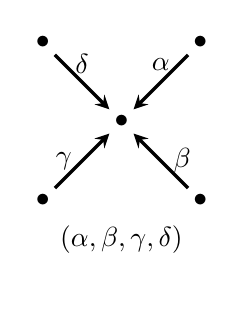
\begin{tikzpicture}[
    every node/.style={circle, draw, fill=black, inner sep=1.5pt, line width=0.5pt}, 
    line width=1.2pt, 
    >=stealth,
    shorten >=0.5pt, 
    shorten <=0.5pt,
    transform shape
]
        % Central node
        \node[draw=none,fill=none] (u) at (0,0) {$\bullet$};
        
        % Surrounding nodes
        \node[draw=none,fill=none] (v1) at (1,1) {$\bullet$};
        \node[draw=none,fill=none] (v2) at (1,-1) {$\bullet$};
        \node[draw=none,fill=none] (v3) at (-1,-1) {$\bullet$};
        \node[draw=none,fill=none] (v4) at (-1,1) {$\bullet$};

        % Edges
        \draw[->] (v1) to node[midway, above, draw=none, fill=none] {\(\alpha\)} (u);
        \draw[->] (v2) to node[midway, right, draw=none, fill=none] {\(\beta\)}(u);
        \draw[->] (v3) to node[midway, left, draw=none, fill=none] {\(\gamma\)} (u);
        \draw[->] (v4) to node[midway, above, draw=none, fill=none] {\(\delta\)} (u);

        \node[draw=none,fill=none] (label) at (0,-1.5) {$(\alpha,\beta,\gamma,\delta)$};
        
    \end{tikzpicture}
    \vspace{-2em}
    \caption{The $4$-star motif.}
    % \vspace{-1em}
    \label{fig:4-star}
\end{wrapfigure}
\textbf{$k$-star motif.} As another example, consider the $k$-star motif :
$$r_1(v_1,u),r_2(v_2,u),\dots,r_k(v_k,u).$$\Cref{fig:4-star} shows an example of $4$-star motif. 
Once again, the set $\gF_n^\text{star}$ of motifs containing all $k$-stars with $k \leq n$ gives us a hierarchy in terms of separation power, where we have that $\gF_n^\text{star} \not\preceq \gF_m^\text{star}$ whenever $n < m$. Hence, every wider star motif adds power for more expressive encodings. 

%: with each larger 
%star motif we get new separation power. 

%\todo{Add an definition of ``path-reverse-permutation'', which, given a 3 path, add all possible reverse permutation up to isomorphism. denote it by some set F\_n path.}


\textbf{A more expressive KGFM.} We also present new ways to improve the $\ultra$ architecture. Adding any motif with $3$ edges to the set of four motifs used in $\ultra$ enhances its expressive power. %We denote this improved architecture as $\mgnn(\gF_3^\text{path})$. 
As an example task shown in \Cref{fig:counter-example}, we show that $\ultra$ with its motifs generates a complete relation graph and fails to distinguish between $r_1$ and $r_2$. In contrast, $\mgnn(\gF_3^\text{path})$ constructs a hyperedge $(r_2, r_3, r_1)$ but not $(r_1, r_3, r_2)$, thereby differentiating between $r_1$ and $r_2$ and solving the task. (See \Cref{app: consequences_mgnn} for detailed proof.)

 
\begin{figure}[t]
\centering
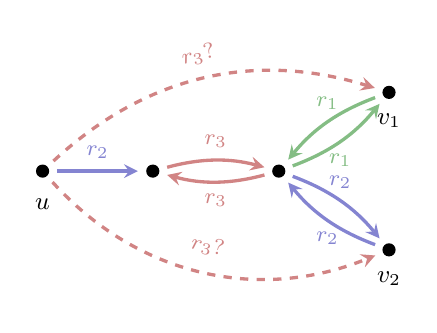
\begin{tikzpicture}[
    every node/.style={circle, draw, fill=black, inner sep=1.5pt, line width=0.5pt}, 
    line width=1.2pt, 
    >=stealth,
    shorten >=3pt, 
    shorten <=3pt,
    transform shape
]
%---------------------------------------------------------------------
% Example color definitions (adjust to taste):
\definecolor{cartoonred}{RGB}{190,80,80}
\definecolor{cartoonblue}{RGB}{80,80,190}
\definecolor{cartoongreen}{RGB}{80,160,80}
\definecolor{cartoonyellow}{RGB}{150,120,0}
%---------------------------------------------------------------------

%--- Node placement with textual labels ---
% The label syntax: label={[font=\small, xshift=<>, yshift=<>]<anchor>:<text>}
% helps you fine-tune positioning around the node.

\node (u)  [label={[font=\small, xshift=0em, yshift=-2em]90:$u$}] at (1,1) {};
\node (m)   at (2.4,1) {};
\node (v2) [label={[font=\small, xshift=0em, yshift=-2em]90:$v_2$}]      at (5.4,0) {};
\node (w)   at (4,1) {};
\node (v1) [label={[font=\small, xshift=0em, yshift=-2em]90:$v_1$}]      at (5.4,2) {};

%--- Self-loops (example) ---
% \draw[->, out=300, in=240, looseness=8] 
%     (v1) to node[right, draw=none, fill=none] {\scriptsize $v_1$} (v1);
% \draw[->, out=300, in=240, looseness=8] 
%     (u) to node[left,  draw=none, fill=none] {\scriptsize $u$} (u);
% \draw[->, out=300, in=240, looseness=8] 
%     (v2) to node[right, draw=none, fill=none] {\scriptsize $v_2$} (v2);

%--- Edges with curved paths and labels ---
% “provide” in blue, “research” in red, etc. are just examples.

% r_1 edges (green):
\draw[->, color=cartoongreen!70, bend right=15] 
    (v1) to node[midway, above, draw=none, fill=none] {\footnotesize $r_1$} (w);
\draw[->, color=cartoongreen!70, bend right=15] 
    (w) to node[midway, below, draw=none, fill=none] {\footnotesize $r_1$} (v1);

% r_2 edges (blue):
\draw[->, color=cartoonblue!70] 
    (u) to node[midway, above, color=cartoonblue!70, draw=none, fill=none] {\footnotesize $r_2$} (m);
\draw[->, color=cartoonblue!70, bend left=15]  
    (w) to node[midway, above, color=cartoonblue!70, draw=none, fill=none] {\footnotesize $r_2$} (v2);
\draw[->, color=cartoonblue!70, bend left=15]  
    (v2) to node[midway, below, color=cartoonblue!70, draw=none, fill=none] {\footnotesize $r_2$} (w);


% r_3 edges (red):
\draw[->, color=cartoonred!70, dashed, bend left=30]  
    (u) to node[midway, above, color=cartoonred!70, draw=none, fill=none, sloped] {\footnotesize $r_3?$} (v1);
\draw[->, color=cartoonred!70, dashed, bend right=35]   
    (u) to node[midway, above, color=cartoonred!70, draw=none, fill=none, sloped] {\footnotesize $r_3?$} (v2);
\draw[->, color=cartoonred!70, bend left=15]  
    (m) to node[midway, above, color=cartoonred!70, draw=none, fill=none] {\footnotesize $r_3$} (w);
\draw[->, color=cartoonred!70, bend left=15]   
    (w) to node[midway, below, color=cartoonred!70, draw=none, fill=none] {\footnotesize $r_3$} (m);

\end{tikzpicture}
\caption{$\ultra$ cannot distinguish between 
\(r_3(u,v_1)\) and \(r_3(u,v_2)\) whereas $\mgnn(\gF_3^{\text{path}})$ can.}
\label{fig:counter-example}
\vspace{-1em}
\end{figure}

Furthermore, the core idea of augmenting existing KGFMs via more expressive motifs to provably enhance their expressivity fits seamlessly in the large bodies of KGFMs in the literature, such as $\ingram$~\citep{ingram}, RMPI~\citep{geng2022relationalmessagepassingfully}, and TRIX~\citep{zhang2024trix}, providing an orthogonal avenue for boosting their expressive power.




\subsection{Comparison with existing link prediction models}

Existing inductive link prediction models, such as $\cmpnn$s and $\text{R-MPNN}$s~\citep{huang2023theory}, can be viewed as special instances of $\mgnn$ with an empty motif set $\emptyset$ and $\init_1$ being a one-hot encoding of relations. However, this configuration breaks relation invariance on relational hypergraphs. %(relation invariance).
% Somewhat counter-intuitively, when treated solely as a node invariant (and not a relation invariant), an instance of $\mgnn$ is inherently \emph{less expressive} than its corresponding entity encoder $\enc_{\text{KG}}$, as it preserves relation invariance. 
Somewhat counter-intuitively, we note that an instance of $\mgnn$ that preserves relation invariance is inherently \emph{less expressive} than its corresponding entity encoder $\enc_{\text{KG}}$, which acts as a node invariant (but not a relation invariant). 
This implies, for example, that NBFNet~\citep{zhu2022neural} is strictly more expressive than $\ultra$ when measured only over graphs with the \emph{same relations types}. This increased expressive power comes at the cost of limited generalization to unseen relations. 
%: while $\mgnn$ can effectively learn functions over relational interactions, the relation embeddings learned by $\enc_{\text{KG}}$ cannot generalize to unseen KGs with different relation vocabularies.


%%%% NOT YET
%%%The \emph{neighborhood} of a node $v\in V$ relative to a relation $r \in R$ is defined as $\mathcal{N}_r(v) := \{u \mid r(u,v) \in E\}$.  





\section{Experimental analysis}
We evaluate $\mgnn$ over a broad range of knowledge graphs to answer the following questions: (\textbf{Q1}) Does $\mgnn$ equipped with more expressive graph motifs exhibit a stronger performance? (\textbf{Q2}) Does $\ultra$ have the same expressive power as $\mgnn(\gF_2^\text{path})$?
(\textbf{Q3}) How does a more refined relation invariant help link prediction tasks?
(\textbf{Q4}) What is the trade-off between expressiveness and scalability for $\mgnn$? (See \Cref{app:scalability,app: complexity}.)
% \begin{enumerate}
%     \item[\textbf{Q1}.] Do $\mgnn$s equipped with more expressive motifs exhibit a stronger performance?
%     \item[\textbf{Q2}.] Does $\ultra$ have the same expressive power as $\mgnn(\gF_2^\text{path})$?
%     \item[\textbf{Q3}.] How does a more refined relation invariant help link prediction tasks?
% \end{enumerate}

In the experiments, we consider a basic architecture which replaces the relation encoder $\enc_\lift$ by HCNet~\citep{huang2024link} and the entity encoder $\enc_{{\rm KG}}$ by a slight modification of NBFNet~\citep{zhu2022neural} (see \Cref{app:mgnn_def}). 




% \begin{table*}[t]
% \centering
% \caption{Accuracy for $\hubclass$ datasets with $\ultra$ and 
% $\mgnn(\gF_m^\text{star})$ with varying $m$. }
%     \label{tab:synthetic}
% \begin{tabular}{cccccccc}
% \toprule
% \multirow{2}{*}{$\hubclass(k)$} & \multirow{2}{*}{$\ultra$} & \multicolumn{6}{c}{$\mgnn(\gF_m^\text{star})$} \\
% \cmidrule{3-8}
%                                 &                           & $m=2$    & $m=3$    & $m=4$    & $m=5$   & $m=6$   & $m=7$   \\
% \midrule
% $k=2$                             &         0.50                 &  0.50    &   \textbf{1.00}   &  -    &  -   &  -   &   -  \\
% $k=3$                             &           0.50                & 0.50     &  0.50    &   \textbf{1.00 }  &  -   &  -   &   -  \\
% $k=4$                             &           0.50               &  0.50    &    0.50  &   0.50   &  \textbf{1.00}   &  -   &   -  \\
% $k=5$                             &             0.50              &  0.50    &   0.50   &   0.50   &  0.50   &   \textbf{1.00}  &  -   \\
% $k=6$                             &               0.50            &  0.50    &    0.50  &   0.50   &  0.50   &  0.50   &  \textbf{1.00}  \\
% \bottomrule
% \end{tabular}
% \end{table*}



\subsection{Synthetic experiments: $\hubclass$}
\label{sec:synthetics}
We construct synthetic datasets $\hubclass(k)$ to validate $\mgnn$'s enhanced expressiveness with richer motifs (\textbf{Q1}).
% We first conduct experiments on synthetic datasets $\hubclass(k)$ to empirically validate that $\mgnn$ with a richer set of motifs is more expressive 
% (\textbf{Q1}). 
% Moreover, we show a strict hierarchy of $\mgnn$ where the model becomes more expressive as we consider motifs involving more relations. 



\textbf{Task \& Setup.} The dataset $\hubclass(k)$ consists of multiple synthetic KGs, where in each KG the relations are partitioned into a \emph{positive} class $P$, a \emph{negative} class $N$, both of size $k+1$, and a query relation $q$.  Each KG contains a $(k+1)$-star \emph{hub} with positive relations, and for each possible subset of relations of $P$ and $N$ of size $k$, the KG contains a positive and negative $k$-star \emph{community}, respectively. An example of such KG is shown in \Cref{fig:hubclass} with $k=2$.
We consider the following classification task: \emph{predict whether there exists a link of relation $q$ from the hub center to positive communities but NOT to negative communities.}  The key to solving this task is successfully differentiating between relations from positive and negative classes.
% 
We consider $\ultra$ and $\mgnn(\gF_m^\text{star})$ for varying $m$, and show the empirical results on these datasets in \Cref{tab:synthetic}. (Further details in \Cref{app:synthetics}.)




\textbf{$\ultra$ \& $\mgnn$ with inexpressive motifs.}
We claim both $\ultra$ and $\mgnn(\gF_m^\text{star})$ with $m \leq k$ cannot solve the task on $\hubclass(k)$. Since the only difference between $P$ and $N$ is the presence of the ($k+1$)-star hub of relations in $P$, these models cannot detect this higher-order motif. Thus, $\lift_\gF(G)$ will contain two disjoint isomorphic hypergraphs: one with positive relations and the other with negative relations. This results in indistinguishability between relations in $P$ and $N$, failing the task. Empirically, we find that $\mgnn(\gF_m^\text{star})$ with $m \leq k$ and $\ultra$ only reach $50\%$ accuracy, no better than a random guess, aligning with our theoretical studies.
%Thus, they will only construct $\lift_\gF(G)$ with two cliques of hyperedges: one among $P$ and the other among $N$, due to the presence of positive and negative communities which consist of star patterns of at most $k$ relations, resulting in indistinguishability between $P$ and $N$ and failing the task. Empirically, we find that $\mgnn(\gF_m^\text{star})$ with $m \leq k$ and $\ultra$ only reach $50\%$ accuracy, no better than a random guess, aligning with our theoretical studies.

\textbf{$\mgnn$ with expressive motifs.} We claim that $\mgnn(\gF_m^\text{star})$ with $m > k$ can detect the presence of the positive hub, precisely due to the additional $(k+1)$-star motifs. This allows the model to construct a hyperedge in $\lift_\gF(G)$ across all relations in $P$, while no such hyperedge exists for $N$, thus distinguishing $P$ from $N$.  Empirically, $\mgnn(\gF_m^\text{star})$ with $m = k+1$ reaches $100\%$ accuracy on $\hubclass(k)$, validating our theoretical results.

\begin{figure}[t]
\centering
% \vspace{-1em}
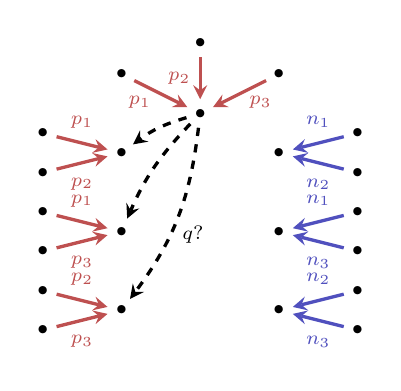
\begin{tikzpicture}[
        every node/.style={circle, draw=none, fill=none, inner sep=2pt, line width=0.5pt, font=\scriptsize}, 
        line width=1.2pt, 
        >=stealth,
        shorten >=-0.5pt, 
        shorten <=-0.5pt,
        transform shape,
        square/.style={regular polygon,regular polygon sides=4},
        triangle/.style={regular polygon,regular polygon sides=3},
    ]
    \definecolor{cartoonred}{RGB}{190,80,80}
    \definecolor{cartoonblue}{RGB}{80,80,190}
    \definecolor{cartoongreen}{RGB}{80,190,80}
    \definecolor{cartoonyellow}{RGB}{190,128,0}
    \definecolor{darkgreen}{RGB}{1, 50, 32}
  \node (A1) at (-1,4) {\(\bullet\)};
  \node (A2) at (0,4.4) {\(\bullet\)};
  \node (A3) at (1,4) {\(\bullet\)};
  \node (B) at (0,3.5) {\(\bullet\)};

  \node (C1) at (-2,3.25) {\(\bullet\)};
  \node (C2) at (-1,3) {\(\bullet\)}; 
  \node (C3) at (2,3.25) {\(\bullet\)};
  \node (C4) at (1,3) {\(\bullet\)};
  
  \node (D1) at (-2,2.75) {\(\bullet\)};
  \node (D2) at (2,2.75) {\(\bullet\)};
  
  \node (E1) at (-2,2.25) {\(\bullet\)};
  \node (E2) at (-1,2) {\(\bullet\)}; 
  \node (E3) at (2,2.25) {\(\bullet\)};
  \node (E4) at (1,2) {\(\bullet\)};
  
  \node (F1) at (-2,1.75) {\(\bullet\)};
  \node (F2) at (2,1.75) {\(\bullet\)};
  
  \node (G1) at (-2,1.25) {\(\bullet\)};
  \node (G2) at (-1,1) {\(\bullet\)};
  \node (G3) at (2,1.25) {\(\bullet\)};
  \node (G4) at (1,1) {\(\bullet\)};
  
  \node (H1) at (-2,0.75) {\(\bullet\)};
  \node (H2) at (2,0.75) {\(\bullet\)};
  
  % Edges with labels
  \draw[->, color=cartoonred] (A1) to node[midway,left, yshift=-0.3em] {\(p_1\)} (B) ;
  \draw[->, color=cartoonred] (A2) to node[midway,left] {\(p_2\)} (B);
  \draw[->, color=cartoonred] (A3) to node[midway, right, yshift=-0.3em] {\(p_3\)} (B) ;
  
  \draw[->, dashed] (B) to[bend right=10]  (C2);
  \draw[->, dashed] (B) to[bend right=10]  (E2);
  \draw[->, dashed] (B) to[bend left=15]  node[midway, below right] {\(q?\)} (G2) ;

  \draw[->, color=cartoonred] (C1) -- (C2) node[midway, above] {\(p_1\)};
  \draw[->, color=cartoonblue] (C3) -- (C4) node[midway, above] {\(n_1\)};
  \draw[->, color=cartoonred] (D1) -- (C2) node[midway, below] {\(p_2\)};
  \draw[->, color=cartoonblue] (D2) -- (C4) node[midway, below] {\(n_2\)};

  \draw[->, color=cartoonred] (E1) -- (E2) node[midway, above] {\(p_1\)};
  \draw[->, color=cartoonblue] (E3) -- (E4) node[midway, above] {\(n_1\)};
  \draw[->, color=cartoonred] (F1) -- (E2) node[midway, below] {\(p_3\)};
  \draw[->, color=cartoonblue] (F2) -- (E4) node[midway, below] {\(n_3\)};

  \draw[->, color=cartoonred] (G1) -- (G2) node[midway, above] {\(p_2\)};
  \draw[->, color=cartoonblue] (G3) -- (G4) node[midway, above] {\(n_2\)};
  \draw[->, color=cartoonred] (H1) -- (G2) node[midway, below] {\(p_3\)};
  \draw[->, color=cartoonblue] (H2) -- (G4) node[midway, below] {\(n_3\)};
  

\end{tikzpicture}
    \vspace{-1em}
    \caption{A example of a KG in one of the synthetic datasets $\hubclass(2)$. Relations in $P$ are in red and $N$ are in blue. 
    % The goal is to predict query $q$ from hub node $u$ to communities center with relations $P$ but not $N$. Correct predictions are shown in dashed.
    }
    \label{fig:hubclass}
    \vspace{-1em}
\end{figure}

\begin{table}[t]
\centering
\caption{Accuracy for $\hubclass(k)$ datasets with $\ultra$ and $\mgnn$ with different $m$-star $\mgnn(\gF_m^\text{star})$ for varying $k$.}
\label{tab:synthetic}
\begin{tabular}{cc|ccccccc}
\toprule
    \multicolumn{2}{c}{$k=?$}        & $\textbf{2}$         & $\textbf{3}$         & $\textbf{4}$         & $\textbf{5}$         & $\textbf{6}$         \\ 
\midrule
% \multicolumn{6}{c}{$\ultra$} \\
\midrule
   \multicolumn{2}{c}{$\ultra$}       & 0.50           & 0.50           & 0.50           & 0.50           & 0.50           \\
% \midrule 
% \multicolumn{6}{l}{$\mgnn(\gF_m^\text{star})$} \\
\midrule
\multirow{6}{*}{$\mgnn$} & $\gF_2^\text{star}$           & 0.50           & 0.50           & 0.50           & 0.50           & 0.50           \\
& $\gF_3^\text{star}$           & \textbf{1.00}  & 0.50           & 0.50           & 0.50           & 0.50           \\
& $\gF_4^\text{star}$           & --             & \textbf{1.00}  & 0.50           & 0.50           & 0.50           \\
& $\gF_5^\text{star}$            & --             & --             & \textbf{1.00}  & 0.50           & 0.50           \\
& $\gF_6^\text{star}$             & --             & --             & --             & \textbf{1.00}  & 0.50           \\
& $\gF_7^\text{star}$            & --             & --             & --             & --             & \textbf{1.00}  \\
\bottomrule
\end{tabular}
\end{table}








\subsection{Pretraining and fine-tuning experiments}
\label{sec:foundational}

\textbf{Datasets \& Evaluations.} For pretraining and fine-tuning experiments, we follow the protocol of \citet{galkin2023ultra} and pretrain on FB15k237~\citep{FB15k237}, WN18RR~\citep{Dettmers2018FB}, and CoDEx Medium~\citep{safavi-koutra-2020-codex}. We then apply zero-shot inference and fine-tuned inference over 51 KGs across three settings: inductive on nodes and relations (\textbf{Inductive} $e,r$), inductive on nodes (\textbf{Inductive} $e$), and \textbf{Transductive}. 
The detailed information of datasets, model architectures, implementations, and hyper-parameters used in the experiments are presented in \Cref{sec:further-experimental-details}.
%
Following convention~\citep{zhu2022neural}, on each knowledge graph and for each triplet $r(u,v)$, we augment the corresponding inverse triplet $r^{-1}(v,u)$ where $r^{-1}$ is a fresh relation symbol. 
% 
For evaluation, we follow \emph{filtered ranking protocol}~\citep{brodes2013transe} and report Mean Reciprocal Rank (MRR), and Hits@10 for each dataset. We report both head and tails prediction results for each triplet on all datasets except three from~\citet{FB15k237-10-20-50}, where only tails prediction results are reported. 
% 
% 
The code is available at \href{https://anonymous.4open.science/r/MOTIF}{https://anonymous.4open.science/r/MOTIF}.




\begin{table*}[t]
\small
\centering
\caption{Average zero-shot and fine-tuned link prediction MRR and Hits@10 over 51 KGs.}
\label{tab:zeroshot}
\begin{tabular}{lccccccc||cc||cc}
\toprule
     & & \multicolumn{2}{c}{\textbf{Inductive $e, r$}} & \multicolumn{2}{c}{\textbf{Inductive $e$}} & \multicolumn{2}{c}{\textbf{Transductive}} & \multicolumn{2}{c}{\textbf{Total Avg}}
     & \multicolumn{2}{c}{\textbf{Pretrained}}\\ 
\textbf{Model} & \textbf{Motif (${\cal F}$)} & \multicolumn{2}{c}{(23 graphs)} & \multicolumn{2}{c}{(18 graphs)} & \multicolumn{2}{c}{(10 graphs)}  & \multicolumn{2}{c}{(51 graphs)} &
\multicolumn{2}{c}{(3 graphs)} 
\\
\cmidrule{3-12}
                && \textbf{MRR}     & \textbf{H@10}    & \textbf{MRR}    & \textbf{H@10}   & \textbf{MRR}    & \textbf{H@10} & \textbf{MRR}    & \textbf{H@10} & \textbf{MRR}    & \textbf{H@10}      \\ 
                      % \midrule
                      \midrule
                      \multicolumn{12}{c}{\textbf{Zero-shot Inference}} \\
                      % \midrule
                      \midrule
$\ultra$ &  &0.345 & 0.513 & 0.431 & 0.566 & 0.339 & 0.494 & 0.374 & 0.529 & -& -\\
% \midrule
% \cmidrule{2-10}
\multirow{4}{*}{\mgnn}  & $\gF_3^\text{path}$ &  \textbf{0.349}        &   \textbf{0.525}       &     \textbf{0.436}       &    \textbf{0.577}  &    \textbf{0.343}         &       \textbf{0.496} &\textbf{0.378} & \textbf{0.537}  & -&  -   \\
& $\gF_2^\text{path}$ & 0.337 & 0.509 & 0.431 & 0.570 & 0.335 & 0.492 & 0.370 & 0.527 &-&-\\
& $\{\textit{h2t}\}$  &    0.330        &     0.503    &      0.422      &  0.559   &    0.325     &   0.482   & 0.361 & 0.518 & -& -\\
& $\emptyset$  &     0.074       &   0.121      &     0.107      & 0.169    &   0.054    &   0.101  & 0.082 & 0.134 & -& -\\
                      \midrule
                      \multicolumn{12}{c}{\textbf{Finetuned Inference}} \\
                      \midrule
     $\ultra$   &   & 0.397 & 0.556 & 0.442 & 0.582 & 0.384 & 0.543 & 0.410 & 0.563 & 0.407& \textbf{0.568}\\
     \mgnn   & $\gF_3^\text{path}$   & \textbf{0.401} & \textbf{0.558} & \textbf{0.455} & \textbf{0.594} & \textbf{0.394} & \textbf{0.549} & \textbf{0.419} & \textbf{0.569} & \textbf{0.415} & 0.565\\
\bottomrule
\end{tabular}
\end{table*}

% \begin{table*}[t]
% \small
% \centering
% \caption{Average zero-shot and fine-tuned link prediction MRR and Hits@10 over 51 KGs.}
% \label{tab:zeroshot}
% \begin{tabular}{lcccccc||cc||cc}
% \toprule
%      & \multicolumn{2}{c}{\textbf{Inductive $e, r$}} & \multicolumn{2}{c}{\textbf{Inductive $e$}} & \multicolumn{2}{c}{\textbf{Transductive}} & \multicolumn{2}{c}{\textbf{Total Avg}}
%      & \multicolumn{2}{c}{\textbf{Pretrained}}\\ 
% \textbf{Model}  & \multicolumn{2}{c}{(23 graphs)} & \multicolumn{2}{c}{(18 graphs)} & \multicolumn{2}{c}{(10 graphs)}  & \multicolumn{2}{c}{(51 graphs)} &
% \multicolumn{2}{c}{(3 graphs)} 
% \\
% \cmidrule{2-11}
%                 & \textbf{MRR}     & \textbf{H@10}    & \textbf{MRR}    & \textbf{H@10}   & \textbf{MRR}    & \textbf{H@10} & \textbf{MRR}    & \textbf{H@10} & \textbf{MRR}    & \textbf{H@10}      \\ 
%                       % \midrule
%                       \midrule
%                       \multicolumn{11}{c}{\textbf{Zero-shot Inference}} \\
%                       % \midrule
%                       \midrule
% $\ultra$   &0.345 & 0.513 & 0.431 & 0.566 & 0.339 & 0.494 & 0.374 & 0.529 & -& -\\
% % \midrule
% % \cmidrule{2-10}
% $\mgnn(\gF_3^\text{path})$ &  \textbf{0.349}        &   \textbf{0.525}       &     \textbf{0.436}       &    \textbf{0.577}  &    \textbf{0.343}         &       \textbf{0.496} &\textbf{0.378} & \textbf{0.537}  & -&  -   \\
% $\mgnn(\gF_2^\text{path})$ & 0.337 & 0.509 & 0.431 & 0.570 & 0.335 & 0.492 & 0.370 & 0.527 &-&-\\
% $\mgnn(\{\textit{h2t}\})$  &    0.330        &     0.503    &      0.422      &  0.559   &    0.325     &   0.482   & 0.361 & 0.518 & -& -\\
% $\mgnn(\emptyset)$  &     0.074       &   0.121      &     0.107      & 0.169    &   0.054    &   0.101  & 0.082 & 0.134 & -& -\\
%                       \midrule
%                       \multicolumn{11}{c}{\textbf{Finetuned Inference}} \\
%                       \midrule
%      $\ultra$      & 0.397 & 0.556 & 0.442 & 0.582 & 0.384 & 0.543 & 0.410 & 0.563 & 0.407& \textbf{0.568}\\
%      $\mgnn(\gF_3^\text{path})$   & \textbf{0.401} & \textbf{0.558} & \textbf{0.455} & \textbf{0.594} & \textbf{0.394} & \textbf{0.549} & \textbf{0.419} & \textbf{0.569} & \textbf{0.415} & 0.565\\
% \bottomrule
% \end{tabular}
% \end{table*}

\textbf{Setup.} To evaluate the impact of graph motifs, we construct four variants of $\mgnn$ models with different $\gF$:  $3$-path ($\gF_3^\text{path}$),  $2$-path ($\gF_2^\text{path}$), $\{\textit{h2t}\}$ only, and no motifs ($\emptyset$), defined in \Cref{sec: expressive_power}. We present the average zero-shot and fine-tuned results of $\mgnn$ over 51 KGs in \Cref{tab:zeroshot}, along with the corresponding results for $\ultra$ taken from \citet{galkin2023ultra}. 
The detailed per-dataset results of pretrained, zero-shot, and finetuned inference are shown in \Cref{app: zeroshot-v1,app: zeroshot-v2,app: finetune-v1,app: finetune-v2}, respectively. Note that in the zero-shot inference setting, \textbf{Inductive} $e,r$, \textbf{Inductive} $e$, and \textbf{Transductive} are in principle indifferent, as all models encounter unseen relations in the inference graph.



% \textbf{Motifs with additional expressive power~(\textbf{Q1}).} 
\textbf{Results.} First of all, note that $\mgnn(\gF_3^\text{path})$ outperforms $\mgnn(\gF_2^\text{path})$ over all 51 datasets on average in zero-shot inference. In the case of fine-tuned inference, a similar trend is present: $\mgnn(\gF_3^\text{path})$ consistently outperforms $\mgnn(\gF_2^\text{path})$. It is also worth noting that both $\mgnn(\gF_3^\text{path})$ and $\mgnn(\gF_2^\text{path})$ achieve further performance improvements after fine-tuning on the training set compared to zero-shot inference. These findings demonstrate that the additionally introduced motifs help the model to learn richer relation invariants (\textbf{Q1}), which are then leveraged for better predictions on new KGs with unseen nodes and relations. This observation is true on both zero-shot and fine-tuned inference.

Secondly, recall that $\mgnn(\gF_2^\text{path})$ and ULTRA have the same expressive power as shown in \Cref{thm: ultra_equiv_motif}.  This theoretical finding is supported in our empirical study, as we see that $\ultra$ performs similarly with $\mgnn(\gF_2^\text{path})$ in these experiments (\textbf{Q2}). 

Lastly, when it comes to comparing $\mgnn(\gF_2^\text{path})$ and $\mgnn(\{\textit{h2t}\})$, we observe a gradual decrease in all metrics on all datasets as the motifs are removed. This aligns with \Cref{thm: theo-necesary-condition}: adding $3$-paths on top of $2$-paths yields more expressive power on $\mgnn$ since there is no core-onto homomorphism from any $2$-path to $3$-path motifs. Similarly, adding $h2h$ or  $t2t$ on top of $h2t$ also yields more expressive power as there is no homomorphism from $h2t$ to $h2h$ or $t2t$. 
% 
In the extreme case, we observe that removing all of the motifs in $\mgnn(\emptyset)$ prevents the model from learning any non-trivial relation invariants, thus exhibiting a complete failure in generalization to unseen KGs.



\subsection{End-to-end experiments}
\label{sec:end-to-end}

% \begin{table*}[t]
% \centering
% \small
% \caption{Average End-to-End link prediction MRR and Hits@10 over 54 KGs.}
% \label{tab:end2end}
% \begin{tabular}{lcccccc||cc}
% \toprule
%      & \multicolumn{2}{c}{\textbf{Inductive $e, r$}} & \multicolumn{2}{c}{\textbf{Inductive $e$}} &  \multicolumn{2}{c}{\textbf{Transductive}} & \multicolumn{2}{c}{\textbf{Total Avg}}  \\ 
% \textbf{Model}  &  \multicolumn{2}{c}{(23 graphs)} & \multicolumn{2}{c}{(18 graphs)}  & \multicolumn{2}{c}{(13 graphs)} & \multicolumn{2}{c}{(54 graphs)}  \\
% \cmidrule{2-9}
%                 & \textbf{MRR}     & \textbf{H@10} & \textbf{MRR}     & \textbf{H@10}    & \textbf{MRR}    & \textbf{H@10}   & \textbf{MRR}    & \textbf{H@10}      \\ 
%                       \midrule
%  \multirow{1}{*}{ULTRA}      &    0.392        &    0.552    &      0.402    &       0.559        & 0.388    &    0.544           &  0.394  & 0.552            \\
% \multirow{1}{*}{$\mgnn$($\gF_3^\text{path}$)}   &    \textbf{0.394}       &    \textbf{0.554}    &    \textbf{0.440}    &  \textbf{0.580}    &    \textbf{0.391}     &   \textbf{0.545}      &     \textbf{0.409}        &  \textbf{0.561}      \\
% \bottomrule
% \end{tabular}
% \end{table*}

% \begin{table}[t]
% \centering
% \small
% \caption{End-to-end MRR and Hits@10 results over 54 KGs.}
% \label{tab:end2end}
% \begin{tabular}{lc||cc}
% \toprule
%      & & \multicolumn{2}{c}{\textbf{Total Avg}}  \\ 
% \textbf{Model}  & \textbf{Motif($\gF$)} & \multicolumn{2}{c}{(54 graphs)}  \\
% \cmidrule{3-4}
%                 & &\textbf{MRR}    & \textbf{H@10}      \\ 
%                       \midrule
%  \multirow{1}{*}{$\ultra$}     &       &  0.394  & 0.552            \\
% \multirow{1}{*}{$\mgnn$} & $\gF_3^\text{path}$    &     \textbf{0.409}        &  \textbf{0.561}      \\
% \bottomrule
% \end{tabular}
% \end{table}

\begin{table}
\centering
\small
\vspace{-1em}
\caption{Average end-to-end MRR and Hits@10 results over 54 KGs.}
\label{tab:end2end}
\begin{tabular}{lcc}
\toprule
     &  \multicolumn{2}{c}{\textbf{Total Avg}}  \\ 
\textbf{Model}  & \multicolumn{2}{c}{(54 graphs)}  \\
\cmidrule{2-3}
                &\textbf{MRR}    & \textbf{H@10}      \\ 
                      \midrule
 \multirow{1}{*}{$\ultra$}           &  0.394  & 0.552            \\
\multirow{1}{*}{$\mgnn(\gF_3^\text{path})$}    &     \textbf{0.409}        &  \textbf{0.561}      \\
\bottomrule
\end{tabular}
\end{table}
We also conduct end-to-end experiments where for each dataset, we train a $\mgnn(\gF_3^\text{path})$ on the training set from scratch and evaluate its corresponding validation and test sets. 
% 
We present the average results over all 54 KGs in \Cref{tab:end2end} (Full results in \Cref{app: end2end-v1} and \Cref{app: end2end-v2}). We continue to see improved performance of $\mgnn(\gF_3^\text{path})$ over $\ultra$ due to the additional motifs, allowing models to capture a richer set of information over relations (\textbf{Q1}). 



\textbf{Degradation of relation learning~(\textbf{Q3}).} 
% 
As a case study, we focus on the end-to-end experiments with WN-v2~\citep{grail2020teru}, an inductive (on node) dataset with only $20$ relations after inverse augmentation. The MRR for $\ultra$ is 0.296, severely lower than that of $\mgnn(\gF_3^\text{path})$ (0.684). To investigate, we plot the cosine similarity\footnote{The block structure is due to the concatenation of augmented inverse relations.} among the computed relation embeddings when queried relations are $r_0 = \textit{derivationally\_related\_form}$ and $r_2=\textit{hypernym}$ in \Cref{fig:cosine}. $\ultra$ produces highly similar relation representations, whereas $\mgnn$ with richer motifs generates distinguishing relation representations, aiding the entity encoder in link prediction.


Nevertheless, we notice that such degradation does not appear in the pretraining experiments, suggesting that either enriching relation learning with diverse motifs or training over multiple KGs could help avoid such degradation.



\begin{figure}
    \centering
    % \vspace{-1em}
    \includegraphics[width=0.7\linewidth]{Image/cosine_similarity.png}
    \caption{Cosine similarities between generated relations embeddings when queried relation $q$ is $r_0$ and $r_2$ in test set of WN-v2.}
    \vspace{-1em}
    \label{fig:cosine}
\end{figure}




% \subsection{Ablation study over equipped motifs}
% \label{sec:ablation-study}




% \begin{table}[t]
% \small
% \centering
% \caption{Ablation study on the number of motifs equipped in MGNN with zero-shot inference.}
% \label{tab:ablation}
% \begin{tabular}{lcccccc||cc}
% \toprule
%      &  \multicolumn{2}{c}{\textbf{Inductive $e, r$}} & \multicolumn{2}{c}{\textbf{Inductive $e$}} & \multicolumn{2}{c}{\textbf{Transductive}} & \multicolumn{2}{c}{\textbf{Total Avg}}  \\ 
% \textbf{Setting} &  \multicolumn{2}{c}{(23 graphs)} & \multicolumn{2}{c}{(18 graphs)} & \multicolumn{2}{c}{(10 graphs)}  & \multicolumn{2}{c}{(51 graphs)}  \\
% \cmidrule{2-9}
%                 & \textbf{MRR}     & \textbf{H@10}    & \textbf{MRR}    & \textbf{H@10}   & \textbf{MRR}    & \textbf{H@10} & \textbf{MRR}    & \textbf{H@10}      \\ 
%                       \midrule
% MGNN  &    0.349        &   0.525       &     0.436       &    0.577  &    0.343         &       0.496 &0.378 & 0.537       \\
% \quad - only $3$-path  & 0.347 & 0.516 & 0.433     &   0.582      &   0.347        &    0.506    & 0.377 & 0.537 \\
% \quad - only $2$-path & 0.337 & 0.509 & 0.431 & 0.570 & 0.335 & 0.492 & 0.370 & 0.527 \\
% \quad - only $h2t$  &    0.330        &     0.503    &      0.422      &  0.559   &    0.325     &   0.482   & 0.361 & 0.518 
% % \\
% % \quad - no relation graph  &     0.074       &   0.121      &     0.107      & 0.169    &   0.054    &   0.101  & 0.082 & 0.134 
% \\
% \bottomrule
% \end{tabular}
% \end{table}




















\section{Conclusions}
We introduced $\mgnn$, a general framework that extends existing KGFMs via incorporating arbitrary motifs. In the context of this framework, we studied the expressive power of KGFMs and identified \emph{sufficient} conditions under which adding new motifs improves $\mgnn$s' ability to compute finer relation invariants. We thoroughly discussed the implications of our results on existing KGFMs. The theoretical findings are empirically validated on a diverse set of datasets. %In particular, we have shown that $\mgnn$ equipped with expressive graph motifs can outperform less expressive KGFMs such as $\ultra$ across a wide range of real-world datasets and tasks. 

Our work provides key insights and concrete recipes for designing more expressive KGFMs. However, the typical trade-off between expressive power and computational complexity clearly also applies to our study. While using richer motifs provably increases $\mgnn$'s expressive power, this may come at the cost of computational efficiency in terms of both time and memory (please see the discussion in \Cref{app:scalability,app: complexity}). A promising avenue for future work is to enhance $\mgnn$'s computational efficiency, thus enabling scalability to real-world large-scale graphs. 

% 
%Empirically, we validate the results via synthetic experiments and a wide range of real-world experiments and show that $\mgnn$ equipped with additional expressive graph motifs outperforms prominent KGFM $\ultra$ across a wide range of real-world datasets and tasks. 

%While adding certain motifs can provably increase $\mgnn$'s expressive power, it also significantly enlarges the relational hypergraphs, impacting computational efficiency in terms of both time and memory (See discussion in \Cref{app:scalability,app: complexity}). A promising future work is to enhance $\mgnn$'s computational efficiency, thus enabling scalability to large-scale real-world applications. Our work provides key insights for designing more expressive KGFMs. 


\clearpage
\section*{Impact Statement}

This paper presents work aimed at advancing the field of Machine Learning. Our methods have potential applications in recommendation systems and knowledge graph completion, among others. While these applications can have significant societal impacts, including improving information retrieval and personalization, as well as potential risks such as bias amplification and misinformation propagation, we do not identify any specific, immediate concerns requiring special attention in this work.


\section*{Acknowledgment}
Bronstein is supported by EPSRC Turing AI World-Leading Research Fellowship No. EP/X040062/1
and EPSRC AI Hub on Mathematical Foundations of Intelligence: An ``Erlangen Programme'' for
AI No. EP/Y028872/1. Reutter is funded by Fondecyt grant 1221799. Barceló and Reutter are
funded by ANID–Millennium Science Initiative Program - CodeICN17002.  Barceló and Romero are funded by the National Center for Artificial
Intelligence CENIA FB210017, BasalANID.



\bibliography{references}
\bibliographystyle{icml2025}


%%%%%%%%%%%%%%%%%%%%%%%%%%%%%%%%%%%%%%%%%%%%%%%%%%%%%%%%%%%%%%%%%%%%%%%%%%%%%%%
%%%%%%%%%%%%%%%%%%%%%%%%%%%%%%%%%%%%%%%%%%%%%%%%%%%%%%%%%%%%%%%%%%%%%%%%%%%%%%%
% APPENDIX
%%%%%%%%%%%%%%%%%%%%%%%%%%%%%%%%%%%%%%%%%%%%%%%%%%%%%%%%%%%%%%%%%%%%%%%%%%%%%%%
%%%%%%%%%%%%%%%%%%%%%%%%%%%%%%%%%%%%%%%%%%%%%%%%%%%%%%%%%%%%%%%%%%%%%%%%%%%%%%%
\newpage
\appendix
\onecolumn


\section{C-MPNNs and HC-MPNNs}
\label{app: C-MPNNs}
In this section, we follow \citet{huang2023theory} and \citet{huang2024link} to define \emph{conditional message passing neural networks} (C-MPNNs) and \emph{hypergraph conditional message passing neural networks} (HC-MPNNs). We then follow \citet{huang2024link} to define
\emph{hypergraph conditional networks} (HCNets) as an architecture from HC-MPNNs. We also present their corresponding relational Weisfeiler Leman test
% and logical formalism 
to study their expressive power rigorously. %These tests will be useful in the coming sections.
For ease of presentation, we omit the discussion regarding history functions and readout functions from \citet{huang2023theory}. Also, some notations are adapted to simplify the exposition.

\subsection{Model definitions}

\textbf{C-MPNNs.} Let $G=(V,E,R)$ be a KG. A \emph{conditional message passing neural network} (C-MPNN) iteratively computes node representations, relative to a fixed query $q\in R$ and a fixed source node $u\in V$, as follows:
\begin{align*}
\vh_{v|u,q}^{(0)} &= \init(u,v,q)\\
\vh_{v|u,q}^{(\ell+1)} &= \update \Big( \vh_{v|u,q}^{(\ell)}, \aggregate(\{\!\! \{ \mes_r(\vh_{w|u,q}^{(\ell)},\vz_q)|~  w \in \mathcal{N}_r(v), r \in R \}\!\!\})\Big), 
\end{align*} 
where $\init$, $\update$, $\aggregate$, and $\mes_r$ are differentiable \emph{initialization}, \emph{update}, \emph{aggregation}, and relation-specific \emph{message} functions, respectively.

We denote by $\vh_q^{(\ell)}:V\times V\to \mathbb{R}^{d(\ell)}$ the function $\vh_q^{(\ell)}(u,v):= \vh_{v|u,q}^{(\ell)}$, and denote $\vz_q$ to be a learnable vector representing the query $q\in R$. We can then interpret a C-MPNN as computing representations of pair of nodes. Given a fixed number of layers $L\geq 0$, a C-MPNN computes the final pair representations as $\vh_q^{(L)}$. In order to decode the likelihood of the fact $q(u,v)$ for some $q \in R$, we consider a unary decoder $\dec: \mathbb{R}^{d(L)}\to  \sR$. We additionally require $\init(u,v,q)$ to satisfy the property of \emph{target node distinguishability}: for all $q \in R$ and $ v \neq u \in V$, it holds that $\init(u,u,q) \neq \init(u,v,q)$.

\textbf{HC-MPNNs.} Given a relational hypergraph $H = (V, E, R)$ and a query $\vq= (q,\tilde{\vu}, t) := q(u_1,\cdots,u_{t-1},?,u_{t+1},\cdots,u_{m})$, for $\ell \geq 0$, an $\hcmpnn$ computes a sequence of feature maps $\vh_{v|\vq}^{(\ell)}$ as follows:
\begin{align*}
\vh_{v|\vq}^{(0)} &= \init(v,\vq), \\
\vh_{v|\vq}^{(\ell+1)}  &=\update\Big( \vh_{v|\vq}^{(\ell)}, \aggregate\big(\vh_{v|\vq}^{(\ell)},  \llbrace \mes_{\rho(e)}\big( \{(\vh_{w|\vq}^{(\ell)}, j ) \mid (w, j) \in \gN_i(e) \}, \vq \big), \mid (e,i) \in E(v) \rrbrace \big)  \Big), 
\end{align*}
where $\init$, $\update$, $\aggregate$, and $\mes_{\rho(e)}$ are differentiable \emph{initialization}, \emph{update}, \emph{aggregation}, and relation-specific \emph{message} functions, respectively. An $\hcmpnn$ has a fixed number of layers $L \geq 0$, and the final
conditional node representations are given by $\vh_{v|\vq}^{(L)} $. 
We denote by $\vh^{(\ell)}_\vq : V \rightarrow \R^{d(\ell)}$ the function $\vh^{(\ell)}_\vq (v) := \vh_{v|\vq}^{(\ell)}$.

\textbf{HCNets.} HCNets can be seen as an architecture of HC-MPNN frameworks by choosing appropriate initialization, aggregation, and message functions. Let $H=(V,E,R)$ be a relational hypergraph. For a query $\vq = (q, \tilde{\vu}, t) := q(u_1,\cdots,u_{t-1},?,u_{t+1},\cdots,u_{m})$, an $\hcnet$ computes the following representations for all $\ell \geq 0$:
\begin{align*}
\vh_{v|\vq}^{(0)} &= \sum_{i \neq t} \mathbbm{1}_{v = u_i} *(\vp_{i} + \vz_q ), \\
\vh_{v|\vq}^{(\ell+1)}  &=\sigma \Big( \mW^{(\ell)}\Big[\vh_{v|\vq}^{(\ell)} \Big\|  \sum_{(e,i) \in E(v) }g_{\rho(e),q}^{(\ell)}\Big(\odot_{j \neq i}(\alpha^{(\ell)}\vh_{e(j)|\vq}^{(\ell)} \!\!+ (1-\alpha^{(\ell)})\vp_{j})  \Big) \Big]
+ \vb^{(\ell)}
\Big), 
\end{align*}
where $g_{\rho(e),q}^{(\ell)}$ is a learnable message function which is often a diagonal matrix, $\sigma$ is an activation function,  $\mW^{(\ell)}$ is a learnable weight matrix, $\vb^{(\ell)}$ as learnable bias term per layer, $\vz_q$ is the learnable query vector for $q \in R$, and $\mathbbm{1}_{C}$ is the indicator function that returns $1$ if condition $C$ is true, and $0$ otherwise. $\alpha$ is a learnable scalar and $\vp_i$ to refer to the sinusoidal positional encoding~\citep{vaswani2023attention} at position $i$. 


\subsection{Relational WL tests}
% \todo{Do I need to include this? double check and see if we need to show this in the proof}
To characterize these models' expressive power, \citet{huang2023theory} and \citet{huang2024link} proposed the corresponding relational Weisfeiler-Leman algorithms to capture these models exactly.

\textbf{Relational assymetric local 2-WL test ($\rawl_2$).}
\label{app:rawl_2}
% 
Following \citet{huang2023theory}, we define the relational asymmetric local 2-WL test ($\rawl_2$) as follows:
Let $G = (V,E,R)$ be a KG and $\eta: V\times V\to D$ an initial pairwise node coloring. We say $\eta$ satisfies \emph{target node distinguishability} if $\eta(u,u)\neq \eta(u,v)$ for all $u\neq v\in V$. Then, for each $\ell\geq 0$, we update the coloring as: 
\begin{align*}
\rdwl_{2}^{(0)}(u,v) & = \eta(u,v), \\
\rdwl_{2}^{(\ell+1)}(u,v) &= {\hash}\big(\rdwl_{2}^{(\ell)}(u,v), \llbrace (\rdwl_{2}^{(\ell)}(u,w), r)\mid w\in \mathcal{N}_r(v), r \in R\rrbrace\big),
\end{align*} 
where $\hash$ injectively maps the above pair to a fresh unique color. It is shown in Theorem 5.1, \citet{huang2023theory} that $\rdwl_{2}^{(\ell)}$ is a relational WL test that characterizes the expressive power of C-MPNNs, i.e., for all C-MPNN, given any knowledge graph $G$, $\ell\geq 0$, we have $\rdwl_{2}^{(\ell)}$ refines the $\ell$ layer of this C-MPNN. In addition, given any knowledge graph $G$, there exists a C-MPNN has equivalent expressive power of $\rdwl_{2}^{(\ell)}$ for all $\ell\geq 0$.

For any knowledge graph $G$, we will sometimes write $\rawl_2^+(G)$ as a shorthand of $\rawl_2(G^+)$, i.e., $\rawl_2$ applied on \emph{augmented knowledge graph} $G^+$. Formally speaking, let $G=(V,E,R)$ be a knowledge graph. Following \citet{huang2023theory}, we define its \emph{augmented knowledge graph} to be $G^+=(V,E^+,R^+)$, where $R^+$ is the disjoint union of $R$ and $R^- := \{r^-\mid r\in R\}$, and 
$E^+ = E \cup E^-$
where $E^-=\{r^{-}(v,u)\mid r(u,v)\in E, u\neq v\}.$

 
\textbf{Hypergraph relational local 1-WL test ($\hrwl_1$).}
\label{app:hrwl}
% 
Similarly, following \citet{huang2024link}, we define the hypergraph relational local 1-WL test ($\hrwl_1$) as follows: Let $H = (V,E,R)$ be a relational hypergraph and $c: V\to D$ an initial node coloring. Then, for each $\ell\geq 0$, we update the coloring as:
\begin{align*}
    \hrwl_1^{(0)}(v) &= c(v), \\
    \hrwl_1^{(\ell+1)}(v) &= \hash \Big( 
    \hrwl_1^{(\ell)}(v), 
    \!\llbrace\big(
            \{ 
                (\hrwl_1^{(\ell)}(w),j) \!\mid (w, j) \in \gN_{i}(e)
            \}, \rho(e)
        \big) \!\mid\! (e,i) \!\in\! E(v)
    \rrbrace
    \Big).
\end{align*}
where the function $\hash$ is an injective mapping that maps the above pair to a unique color that has not been used in the previous iteration.
When we restrict $\hrwl_1$ to initial colorings $c$ that respect a given query $\vq := (q,\tilde{\vu},t) = q(u_1,\cdots,u_{t-1},u_{t+1},\cdots,u_k)$, we say that the coloring $c$ satisfies \emph{generalized target node distinguishability with respect to $\vq$} if:
\begin{align*}
    c(u) \neq c(v) \quad \forall u \in \tilde{\vu}, v \notin \tilde{\vu} \qquad  \text{and} \qquad 
    c(u_i) \neq c(u_j) \quad \forall u_i, u_j \in \tilde{\vu}, u_i \neq u_j.
\end{align*}
Then, Theorem 5.1, \citet{huang2024link} shows that $\hrwl_1$ with initial coloring $c$ satisfying \emph{generalized target node distinguishability} characterizes the expressive power of HC-MPNNs. 

\textbf{Hypergraph relational local 2-WL test ($\hcwl_2$).} Following \citet{huang2024link}, if we further restrict the test and apply only on knowledge graphs where all the edges have arity $2$ and additionally only with tail prediction, we can instead assign pair-wise coloring $\eta : V \times V \mapsto D$ satisfying \emph{target node distinguishability}, i.e. $\forall u \neq v, \eta(u,u) \neq \eta(u,v)$. Then, we define a \emph{relational hypergraph conditioned local 2-WL test}, denoted as $\hcwl_2$. $\hcwl_2$ iteratively updates binary coloring $\eta$ as follow for all $\ell \geq 0$:
\begin{align*}
   \hcwl_2^{(0)} &= \eta(u,v) \\
   \hcwl_2^{(\ell+1)}(u,v) &= \hash \Big( 
   \hcwl_2^{(\ell)}(u,v), \llbrace \big( 
           \{ 
               (\hcwl_2^{(\ell)}(u, w),j) \!\mid\! (w, j) \!\in\! \gN_{i}(e)
           \},
       \rho(e)
       \big) \mid (e,i) \in E(v) \rrbrace
   \Big)
\end{align*}


\section{A WL test for $\mgnn$}
\label{app:test-motif}

We start by introducing a two-stage WL test that matches the separating power of $\mgnn({\cal F})$, for a set of motifs ${\cal F}$. Using this equivalence, we show Proposition \ref{prop:same_expressive} and Theorem \ref{thm: theo-necesary-condition}, in sections \ref{app:same_expressive} and \ref{app:theo-necesary-condition}, respectively. Characterizing the separating power of $\mgnn({\cal F})$ via a suitable test, allows us to reason about simpler coloring schemes, which, in turn, makes the proofs more manageable. Also, the equivalence between $\mgnn({\cal F})$ and our two-stage WL test may be of independent interest. 



We assume a given KG $G=(V,E,R)$. Our test assigns one color to each link $q(u,v)$, for $q\in R$ and $u,v\in V$ (recall that links are not necessarily facts in $G$). In the first stage, we color the nodes of 
$\lift_{{\cal F}}(G)=(V_\lift,E_\lift,R_\lift)$, that is, the set $V_\lift=R$. When coloring a relation $r\in R$, we always condition on another relation $q\in R$. We denote by $\hcwl_{{\cal F}}^{(t)}(q,r)$ the color assigned to $r$, conditioned on $q$, on iteration $t\geq 0$. We assume a predefined number of iterations $T\geq 0$, which will be a parameter of our test. In the second stage, we color the nodes $v$ of the KG $G$, conditioned on a relation $q\in R$ and a source node $u\in V$. This determines the final color $\tcolor_{{\cal F}, T}^{(\ell)}(q(u,v))$ for the link $q(u,v)$. Crucially, the second stage relies on the first stage in that it uses the colors $\hcwl_{{\cal F}}^{(T)}(q,r)$ internally. Roughly speaking, the first-stage coloring follows the coloring strategy of $\hrwl_1$ applied to $\lift_{\cal F}(G)$, while the second-stage coloring follows the strategy of $\rawl_2$, after incorporating the relation encodings obtained in the first stage. (see Section \ref{app: C-MPNNs} for the definition of $\hrwl_1$ and $\rawl_2$). 

Formally, the first-stage colors $\hcwl_{{\cal F}}^{(t)}$ are defined via the following rules:
\begin{align*}
    \hcwl_{{\cal F}}^{(0)}(q,r) & = \mathbbm{1}_{r = q} * 1\\
    \hcwl_{{\cal F}}^{(t+1)}(q,r) & = \hash\Big( \hcwl_{{\cal F}}^{(t)}(q,r), 
     \llbrace \big(\{(\hcwl_{{\cal F}}^{(t)}(q,s), j ) \mid 
(s,j) \in \gN^i(e) \}, \rho(e) \big) \mid (e,i) \in E_{\lift}(r) \rrbrace \Big).
\end{align*}
Recall that 
$$E_{\lift}(r) = 
  \left\{
    (e,i) \mid  e(i)=r, e \in E_\lift, 1 \leq i \leq \mathtt{ar}(\rho(e))
    \right\}.$$
    is the set of edge-position pairs of a node $r$, and $\gN^{i}{(e)}$ is the positional neighborhood of a hyperedge $e$ with respect to a position $i$: $$\gN^{i}(e)=
    \left\{
    (e(j),j) \mid  j \neq i,  1 \leq j \leq \mathtt{ar}(\rho(e))
    \right\}.$$

$\mathbbm{1}_{r = q}$ takes value $1$ if $r=q$, and $0$ otherwise. The function $\hash$ is a fixed injective function taking values in the natural numbers. 

The second-stage colors $\tcolor_{{\cal F}, T}^{(\ell)}$, where $T\geq 0$ is a parameter, are defined via the following rules:
\begin{align*}
    \tcolor_{{\cal F}, T}^{(0)}(q(u,v)) & = \mathbbm{1}_{v = u} * \hcwl_{{\cal F}}^{(T)}(q,q)\\
   \tcolor_{{\cal F}, T}^{(\ell+1)}(q(u,v)) & = \hash\Big(\tcolor_{{\cal F}, T}^{(\ell)}(q(u,v)), \llbrace \big(\tcolor_{{\cal F}, T}^{(\ell)}(q(u,w)),\hcwl_{{\cal F}}^{(T)}(q,r)\big)\mid w \in \mathcal{N}_r(v), r \in R \rrbrace \Big). 
\end{align*}

We start by showing that our coloring scheme upper bounds the separation power of any model in $\mgnn({\cal F})$. For simplicity, we assume that any model in $\mgnn({\cal F})$ has the form $(\enc_{{\rm KG}},(\gF,\enc_\lift))$, where 
\begin{enumerate}
\item the initialization function $\init_1$ used by the relational encoder $\enc_\lift$ is defined as $\init_1(q,r) = \mathbbm{1}_{r = q} * \mathbf{1}^d$, and 
\item the initialization function $\init_2$ used by the entity encoder is defined as $\init_2(u,v,q) = \mathbbm{1}_{v = u} *\vh_{q|q}^{(T)}$. 
\end{enumerate}
This is a common choice, and in particular, it is the choice we take in our basic architecture for the experiments (see Section \ref{app:mgnn_def}). 

\begin{proposition}
\label{app:upperbound-test}
Let $G=(V,E,R)$ be a KG and $(\enc_{{\rm KG}},(\gF,\enc_\lift))$ be a $\mgnn({\cal F})$ instance, where $\enc_\lift$ and $\enc_{{\rm KG}}$ involve $T\geq 0$ and $L\geq 0$ layers, respectively. Then for every pair of links $q(u,v)$ and $q'(u',v')$, we have that
$$\col_{{\cal F},T}^{(L)}(q(u,v)) = \col_{{\cal F},T}^{(L)}(q'(u',v')) \implies \enc_{{\rm KG},u,q}[v] = \enc_{{\rm KG},u',q'}[v'].$$
\end{proposition}

\begin{proof}
We show first the following claim:

($\dagger$) for every quadruple of relations $q,r,q',r'\in R$, we have that
$$\hcwl_{{\cal F}}^{(T)}(q,r) = \hcwl_{{\cal F}}^{(T)}(q',r') \implies \enc_{\lift,q}[r] = \enc_{\lift,q'}[r'].$$

Recall that $\enc_{\lift,p}[s]$ is determined by the sequence of vectors $\vh_{s|p}^{(t)}$ and that $\enc_{\lift,p}[s]= \vh_{s|p}^{(T)}$. 

Take a quadruple $q,r,q',r'\in R$. We prove by induction that for every $0\leq t\leq T$, we have that 
$$\hcwl_{{\cal F}}^{(t)}(q,r) = \hcwl_{{\cal F}}^{(t)}(q',r') \implies \vh_{r|q}^{(t)} = \vh_{r'|q'}^{(t)}.$$

For the base case, take $t=0$. Assume that $\hcwl_{{\cal F}}^{(0)}(q,r) = \hcwl_{{\cal F}}^{(0)}(q',r')$. By the definition of $\hcwl_{{\cal F}}^{(0)}$, either $q=r$ and $q'=r'$, or $q\neq r$ and $q'\neq r'$. In either case, we obtain $\vh_{r|q}^{(0)} = \mathbbm{1}_{r = q} * \mathbf{1}^d = \mathbbm{1}_{r' = q'} * \mathbf{1}^d=\vh_{r'|q'}^{(0)}$. 

For the inductive case, suppose that 
$$\hcwl_{{\cal F}}^{(t)}(q,r) = \hcwl_{{\cal F}}^{(t)}(q',r') \implies \vh_{r|q}^{(t)} = \vh_{r'|q'}^{(t)}$$
and assume that $\hcwl_{{\cal F}}^{(t+1)}(q,r) = \hcwl_{{\cal F}}^{(t+1)}(q',r')$. By the definition of $\hcwl_{{\cal F}}$, it follows that
\begin{align*}
\hcwl_{{\cal F}}^{(t)}(q,r) & = \hcwl_{{\cal F}}^{(t)}(q',r') \\
\llbrace \big(\{(\hcwl_{{\cal F}}^{(t)}(q,s), j ) \mid 
(s,j) \in \gN^i(e) \}, \rho(e) \big) \mid (e,i) \in E_{\lift}(r) \rrbrace & =\\
\llbrace \big(\{(\hcwl_{{\cal F}}^{(t)}(q',s'), j ) & \mid 
(s',j) \in \gN^i(e) \}, \rho(e) \big) \mid (e,i) \in E_{\lift}(r') \rrbrace.
\end{align*}
We can apply the inductive hypothesis to the first equation and obtain that $\vh_{r|q}^{(t)} = \vh_{r'|q'}^{(t)}$. The second equation together with the inductive hypothesis implies that 
\begin{align*}
\llbrace \big(\{(\vh_{s|q}^{(t)}, j ) \mid 
(s,j) \in \gN^i(e) \}, \rho(e) \big) \mid (e,i) \in E_{\lift}(r) \rrbrace & =\\
\llbrace \big(\{(\vh_{s'|q'}^{(t)}, j ) & \mid 
(s',j) \in \gN^i(e) \}, \rho(e) \big) \mid (e,i) \in E_{\lift}(r') \rrbrace.
\end{align*}
As a consequence, we have that
\begin{align*}
M = \llbrace \mes_{\rho(e)} \big(\{(\vh_{s|q}^{(t)}, j ) \mid 
(s,j) \in \gN^i(e) \} \big) \mid (e,i) \in E_{\lift}(r) \rrbrace & = \\
\llbrace \mes_{\rho(e)} \big(\{(\vh_{s'|q}^{(t)}, j ) & \mid 
(s',j) \in \gN^i(e) \} \big) \mid (e,i) \in E_{\lift}(r) \rrbrace = M'
\end{align*}
where $\mes_{\rho(e)}$ is the motif-specific message function used in the $(t+1)$-th layer. It follows that 
$$\vh_{r|q}^{(t+1)} = \update_1 \big( \vh_{r|q}^{(t)},  \aggregate_1(M) \big) =  \update_1 \big( \vh_{r'|q'}^{(t)},  \aggregate_1(M') \big) =  \vh_{r'|q'}^{(t+1)}$$
as required. ($\update_1$ and $\aggregate_1$ are the update and aggregate functions in the $(t+1)$-th layer.)

Take a pair of links $q(u,v)$ and $q'(u',v')$. Now we are ready to show 
$$\col_{{\cal F},T}^{(L)}(q(u,v)) = \col_{{\cal F},T}^{(L)}(q'(u',v')) \implies \enc_{{\rm KG},u,q}[v] = \enc_{{\rm KG},u',q'}[v'].$$
Recall that $\enc_{{\rm KG},x,p}[y]$ is determined by the sequence of vectors $\vh_{y|x,p}^{(\ell)}$ and that $\enc_{{\rm KG},x,p}[y]=\vh_{y|x,p}^{(L)}$.

We show by induction that for every $0\leq \ell\leq L$, it holds that
$$\col_{{\cal F},T}^{(\ell)}(q(u,v)) = \col_{{\cal F},T}^{(\ell)}(q'(u',v')) \implies \vh_{v|u,q}^{(\ell)} = \vh_{v'|u',q'}^{(\ell)}.$$

In the base case $\ell=0$. Suppose $\col_{{\cal F},T}^{(0)}(q(u,v)) = \col_{{\cal F},T}^{(0)}(q'(u',v'))$, i.e.,  $\mathbbm{1}_{v = u} * \hcwl_{{\cal F}}^{(T)}(q,q) = \mathbbm{1}_{v' = u'} * \hcwl_{{\cal F}}^{(T)}(q',q')$. Note that without loss of generality, we can assume that $\hash$ never takes the value $0$, and hence $\hcwl_{{\cal F}}^{(T)}(q,q)\neq 0$ and $\hcwl_{{\cal F}}^{(T)}(q',q')\neq 0$. We then have two cases:
\begin{enumerate}
\item $v\neq u$ and $v'\neq u'$. We obtain $\vh_{v|u,q}^{(0)} = \vh_{v'|u',q'}^{(0)}$ as required.
\item $v= u$, $v'= u'$ and $\hcwl_{{\cal F}}^{(T)}(q,q) = \hcwl_{{\cal F}}^{(T)}(q',q')$. By the claim ($\dagger$), we have that $\vh_{q|q}^{(T)} = \vh_{q'|q'}^{(T)}$. We conclude that $\vh_{v|u,q}^{(0)} = \vh_{v'|u',q'}^{(0)}$ as desired.
\end{enumerate}

For the inductive step, suppose that 
$$\col_{{\cal F},T}^{(\ell)}(q(u,v)) = \col_{{\cal F},T}^{(\ell)}(q'(u',v')) \implies \vh_{v|u,q}^{(\ell)} = \vh_{v'|u',q'}^{(\ell)}.$$
Assume that $\col_{{\cal F},T}^{(\ell+1)}(q(u,v)) = \col_{{\cal F},T}^{(\ell+1)}(q'(u',v'))$. It follows that
\begin{align*}
\col_{{\cal F},T}^{(\ell)}(q(u,v)) & = \col_{{\cal F},T}^{(\ell)}(q'(u',v'))\\
 \llbrace \big(\tcolor_{{\cal F}, T}^{(\ell)}(q(u,w)),\hcwl_{{\cal F}}^{(T)}(q,r)\big)\mid w \in \mathcal{N}_r(v), r \in R \rrbrace & =  \llbrace \big(\tcolor_{{\cal F}, T}^{(\ell)}(q'(u',w)),\hcwl_{{\cal F}}^{(T)}(q',r)\big)\mid w \in \mathcal{N}_r(v'), r \in R \rrbrace. 
\end{align*}

Using the inductive hypothesis and claim ($\dagger$), we obtain that 
\begin{align*}
\vh_{v|u,q}^{(\ell)} & = \vh_{v'|u',q'}^{(\ell)}\\
 \llbrace \big(\vh_{w|u,q}^{(\ell)},\vh_{r|q}^{(T)}\big)\mid w \in \mathcal{N}_r(v), r \in R \rrbrace & =  \llbrace \big(\vh_{w|u',q'}^{(\ell)},\vh_{r|q'}^{(T)}\big)\mid w \in \mathcal{N}_r(v'), r \in R \rrbrace. 
\end{align*}
It follows that 
 $$ N = \llbrace \mes\big(\vh_{w|u,q}^{(\ell)},\enc_{\lift,q}[r]\big)\mid w \in \mathcal{N}_r(v), r \in R \rrbrace  =  \llbrace \mes\big(\vh_{w|u',q'}^{(\ell)},\enc_{\lift,q'}[r]\big)\mid w \in \mathcal{N}_r(v'), r \in R \rrbrace = N'.$$
 We conclude that 
 $$\vh_{v|u,q}^{(\ell+1)} = \update_2 \big( \vh_{v|u,q}^{(\ell)},  \aggregate_2(N) \big) =  \update_2 \big( \vh_{v'|u',q'}^{(\ell)},  \aggregate_2(N') \big) =  \vh_{v'|u',q'}^{(\ell+1)}.$$
as required. ($\update_2$ and $\aggregate_2$ are the update and aggregate functions in the $(\ell+1)$-th layer.)
\end{proof}

We now show that $\mgnn({\cal F})$ can be as powerful as our test, regarding separating links. %We exploit results from \citet{huang2023theory, huang2024link}.
%In \citet{huang2024link}, a WL test called $\hrwl$ was introduced to capture the power of distinguishing nodes of HR-MPNNs, which are models that produce node representations over relational hypergraphs. For formal definitions, see \Cref{app: C-MPNNs}. %As it turns out, our first-stage  coloring scheme $\hcwl$ can be alternatively defined as the coloring $\hrwl$ applied to a suitable relational hypergraph we defined next. 

\begin{proposition}
\label{app:lowerbound-test}
Let $G=(V,E,R)$ be a KG, and let $T,L\geq 0$ be natural numbers. Then there exists an instance  $(\enc_{{\rm KG}},(\gF,\enc_\lift))$ of $\mgnn({\cal F})$ such that for every pair of links $q(u,v)$ and $q'(u',v')$, we have that
$$\col_{{\cal F},T}^{(L)}(q(u,v)) = \col_{{\cal F},T}^{(L)}(q'(u',v')) \iff \enc_{{\rm KG},u,q}[v] = \enc_{{\rm KG},u',q'}[v'].$$
\end{proposition}

\begin{proof}
It suffices to choose $(\enc_{{\rm KG}},(\gF,\enc_\lift))$ such that the functions $\update_1^{(t)}$, $\aggregate_1^{(t)}$ and $\mes_{\rho(e)}^{(t)}$ defining $\enc_\lift$, and the functions $\update_2^{(\ell)}$, $\aggregate_2^{(\ell)}$ and $\mes^{(\ell)}$ defining $\enc_{{\rm KG}}$, are injective. Indeed, suppose this condition holds. We prove first by induction that for every $q,r,q',r'\in R$ and $0\leq t\leq T$, 
$$\vh_{r|q}^{(t)} = \vh_{r'|q'}^{(t)}\implies \hcwl_{{\cal F}}^{(t)}(q,r) = \hcwl_{{\cal F}}^{(t)}(q',r').$$
For $t=0$, the result follows by our assumption on $\init_1$. Suppose that $\vh_{r|q}^{(t+1)} = \vh_{r'|q'}^{(t+1)}$. As $\update_1^{(t)}$ is injective, we have that $\vh_{r|q}^{(t)} = \vh_{r'|q'}^{(t)}$ and $\aggregate_1^{(t)}(M) = \aggregate_1^{(t)}(M')$. From the former and by induction, we obtain $\hcwl_{{\cal F}}^{(t)}(q,r) = \hcwl_{{\cal F}}^{(t)}(q',r')$. From the later, as  $\aggregate_1^{(t)}$ is injective, we obtain $M=M'$. Using the fact that $\mes_{\rho(e)}^{(t)}$ is injective, we conclude that 
$$\llbrace \{(\vh_{s|q}^{(t)}, j ) \mid 
(s,j) \in \gN^i(e) \}  \mid (e,i) \in E_{\lift}(r) \rrbrace = \llbrace \{(\vh_{s|q'}^{(t)}, j ) \mid 
(s,j) \in \gN^i(e) \}  \mid (e,i) \in E_{\lift}(r') \rrbrace.$$
By induction, we have
$$\llbrace \{(\hcwl_{{\cal F}}^{(t)}(q,s), j ) \mid 
(s,j) \in \gN^i(e) \}  \mid (e,i) \in E_{\lift}(r) \rrbrace = \llbrace \{(\hcwl_{{\cal F}}^{(t)}(q',s), j ) \mid 
(s,j) \in \gN^i(e) \}  \mid (e,i) \in E_{\lift}(r') \rrbrace.$$
This implies that $\hcwl_{{\cal F}}^{(t+1)}(q,r) = \hcwl_{{\cal F}}^{(t+1)}(q',r')$ as required. 
Now we prove by induction that for every pair of links $q(u,v)$ and $q'(u',v')$, and $0\leq \ell \leq L$, it holds that
$$\vh_{v|u,q}^{(\ell)} = \vh_{v'|u',q'}^{(\ell)}\implies \col_{{\cal F},T}^{(\ell)}(q(u,v)) = \col_{{\cal F},T}^{(\ell)}(q'(u',v')).$$
Note that this implies that 
$$\col_{{\cal F},T}^{(L)}(q(u,v)) = \col_{{\cal F},T}^{(L)}(q'(u',v')) \iff \enc_{{\rm KG},u,q}[v] = \enc_{{\rm KG},u',q'}[v'].$$
The implication holds for $\ell=0$ by the assumption on $\init_2$ and the fact that $\vh_{q|q}^{(T)}=\vh_{q'|q'}^{(T)}\implies \hcwl_{{\cal F}}^{(T)}(q,q) = \hcwl_{{\cal F}}^{(T)}(q',q')$.
Assume that $\vh_{v|u,q}^{(\ell+1)} = \vh_{v'|u',q'}^{(\ell+1)}$. As $\update_2^{(t)}$ is injective, we have that $\vh_{v|u,q}^{(\ell)} = \vh_{v'|u',q'}^{(\ell)}$ and $\aggregate_2^{(\ell)}(N) = \aggregate_2^{(\ell)}(N')$. From the former and by induction, we obtain $\col_{{\cal F},T}^{(\ell)}(q(u,v)) = \col_{{\cal F},T}^{(\ell)}(q'(u',v'))$. From the later, since  $\aggregate_2^{(\ell)}$ is injective, we have $N=N'$. As $\mes^{(\ell)}$ is injective, we obtain that 
$$ \llbrace \big(\vh_{w|u,q}^{(\ell)},\vh_{r|q}^{(T)}\big)\mid w \in \mathcal{N}_r(v), r \in R \rrbrace =  \llbrace \big(\vh_{w|u',q'}^{(\ell)},\vh_{r|q'}^{(T)}\big)\mid w \in \mathcal{N}_r(v'), r \in R \rrbrace.$$ 
By induction, we have
$$ \llbrace \big(\col_{{\cal F},T}^{(\ell)}(q(u,v)),\hcwl_{{\cal F}}^{(T)}(q,r)\big)\mid w \in \mathcal{N}_r(v), r \in R \rrbrace =  \llbrace \big(\col_{{\cal F},T}^{(\ell)}(q'(u',v')),\hcwl_{{\cal F}}^{(T)}(q',r)\big)\mid w \in \mathcal{N}_r(v'), r \in R \rrbrace.$$ 
This implies that $\col_{{\cal F},T}^{(\ell+1)}(q(u,v)) = \col_{{\cal F},T}^{(\ell+1)}(q'(u',v'))$ as desired. 

It is easy to find injective funtions $\update_1^{(t)}$, $\aggregate_1^{(t)}$,  $\mes_{\rho(e)}^{(t)}$, $\update_2^{(\ell)}$, $\aggregate_2^{(\ell)}$, $\mes^{(\ell)}$. For instance $\update_1^{(t)}$ and $\update_2^{(\ell)}$ can be vector concatenation, and $\aggregate_1^{(t)}$,  $\mes_{\rho(e)}^{(t)}$, $\aggregate_2^{(\ell)}$, $\mes^{(\ell)}$ can be chosen using Lemma 5 from \citet{xu2018how} (see also Lemma VIII.5 from \citet{GroheLogicGNN}). Another alternative is to choose $\update_1^{(t)}$, $\aggregate_1^{(t)}$,  $\mes_{\rho(e)}^{(t)}$ according to Theorem 4.1 in \citet{huang2024link}, and $\update_2^{(\ell)}$, $\aggregate_2^{(\ell)}$, $\mes^{(\ell)}$ according to Theorem 5.1 in \citet{huang2023theory}.

%We start by providing an alternative definition of $\hcwl$ in terms of $\hrwl$, defined in section \ref{app: C-MPNNs}. Define the relational hypergraph %$\lift_{{\cal F}}^2(G)=(V_{\lift}\times V_{\lift}, E^2_{\lift}, R_{\lift})$, where
%$$E^2_{\lift} = \{P((q,r_1),\dots, (q,r_n))\mid P(r_1,\dots, r_n)\in E_{\lift}, q\in R\}.$$
%That is, the nodes of $\lift_{{\cal F}}^2(G)$ are \emph{pairs} of relations $(q,r)\in R\times R$.  The relation types are the same as in $\lift_{{\cal F}}(G)$, namely, the set of motifs $R_{\lift}$. For the set of facts of $\lift_{{\cal F}}^2(G)$, for each fact $P(r_1,\dots, r_n)$ in $\lift_{{\cal F}}(G)$ and each $q\in R$, we have a fact of the form $P((q,r_1),\dots, (q,r_n))$ in $\lift_{{\cal F}}^2(G)$. Then, by definition, we have 
%$$\hcwl_{{\cal F}}^{(t)}(q,r)=\hrwl^{(t)}((q,r), \lift_{{\cal F}}^2(G)),$$
%for every $0\leq t\leq T$, assuming we define $\hrwl^{(0)}((q,r), \lift_{{\cal F}}^2(G))=\hcwl_{{\cal F}}^{(0)}(q,r)$.

%We can apply Proposition \ref{} to $\lift_{{\cal F}}^2(G)$ and the initial coloring $\hrwl^{(0)}((q,r), \lift_{{\cal F}}^2(G))=\hcwl_{{\cal F}}^{(0)}(q,r)$, to obtain a HR-MPNN model ${\cal A}$ such that for every quadruple $q,r,q',r'\in R$, it holds that
%$$ \hrwl^{(T)}((q,r), \lift_{{\cal F}}^2(G)) = \hrwl^{(T)}((q',r'), \lift_{{\cal F}}^2(G)) \iff {\cal A}((q,r), \lift_{{\cal F}}^2(G)) = {\cal A}((q',r'), \lift_{{\cal F}}^2(G)).$$
%Note that, by definition of  HR-MPNNs shown in \Cref{app: C-MPNNs}, we can use the model ${\cal A}$ to directly define an equivalent relation encoder $({\cal F}, \enc_\lift)$ in $\mgnn({\cal F})$. The relation encoder is equivalent in the sense that
%$$\enc_{\lift,q}[r] = {\cal A}((q,r), \lift_{{\cal F}}^2(G))$$
%holds for every $q,r\in R$.
%Putting things together, we conclude that for every quadruple $q,r,q',r'\in R$, 
%$$ \hcwl_{\cal F}^{(T)}(q,r) = \hcwl_{\cal F}^{(T)}(q',r') \iff \enc_{\lift,q}[r] = \enc_{\lift,q'}[r'].$$
%In other words, we found a relation encoder simulating the first stage of our test. 

%Let $q\in R$. Define the KG $G_q=(V, E_q, R_q)$, where $R_q$ is obtained from $R$ by renaming each $r\in R$ to $r'=\hcwl_{{\cal F}}^{(T)}(q,r)$, and $E_q$ is obtained from $E$ by applying this renaming, that is, replacing each fact $r(u,v)$ by $r'(u,v)$. By construction, we have that for every $u,v\in V$ and $0\leq \ell\leq L$,  
%$$\rawl^{(\ell)}(u,v,G_q) = \col_{{\cal F}, T}^{(\ell)}(q(u,v)),$$
%assuming that $\rawl^{(0)}(u,v,G_q) = \mathbbm{1}_{v = u} * \hcwl_{{\cal F}}^{(T)}(q,q) = \col_{{\cal F}, T}^{(0)}(q(u,v))$. On the other hand, we can apply Proposition \ref{} to the KG $G_q$ and initial pairwise node coloring $\rawl^{(0)}(u,v,G_q) = \col_{{\cal F}, T}^{(0)}(q(u,v))$ and obtain a C-MPNN model ${\cal B}_q$ such that for every quadruple $u,v,u',v'\in V$, 
%$$\rawl^{(L)}(u,v, G_q) = \rawl^{(L)}(u',v', G_q) \iff {\cal B}_q(u,v, G_q) = {\cal B}_q(u,v, G_q)$$
\end{proof}

As a direct corollary of Propositions \ref{app:upperbound-test} and \ref{app:lowerbound-test}, we obtain:

\begin{corollary}
\label{app:coro-test}
Let ${\cal F}$ and ${\cal F}'$ be two set of motifs. Then ${\cal F}\preceq {\cal F}'$ if and only if for every KG $G=(V,E,R)$ and link $q(u,v)$, $q'(u',v')$, whenever $\col_{{\cal F}, T}^{(L)}(q(u,v))=\col_{{\cal F}, T}^{(L)}(q'(u',v'))$ for every $T,L\geq 0$, then $\col_{{\cal F'}, T}^{(L)}(q(u,v))=\col_{{\cal F'}, T}^{(L)}(q'(u',v'))$ for every $T,L\geq 0$. 
\end{corollary}

\section{Missing proofs in the paper}

\subsection{Proof of Proposition \ref{prop:same_expressive}}
\label{app:same_expressive}
\emph{
Let
$P = (G_M,\bar r)$ and  $P' = (G_M',\bar r')$ be two graph motifs such that $G_M$ is isomorphic to $G_M'$. Then, for any set $\F$ of graph motifs:  
$$(\F \cup\{P\}) \, \sim \, (\F \cup\{P'\}) \, \sim \, (\F \cup\{P,P'\}).$$}

\begin{proof}
We only show that $(\F \cup\{P\}) \sim 
(\F \cup\{P,P'\})$, the part that $(\F \cup\{P\}) \sim 
(\F \cup\{P'\})$ is analogous. 

For readability, let us write $\F_1 = \F \cup\{P\}$ and $\F_2 = \F \cup\{P,P'\}$. 
Further, $E_1$ and $E_2$ correspond to the edges of $\lift_{\F_1}(G)$ and $\lift_{\F_2}(G)$, respectively. 

We make use of Corollary \ref{app:coro-test}, 
and show that for every KG $G=(V,E,R)$, every pair of links $q(u,v), q'(u',v')$ and every $T,L\geq 0$, 
$$\col_{{\cal F}_1,T}^{(L)}(q(u,v)) = \col_{{\cal F}_1,T}^{(L)}(q(u',v')) \iff \col_{{\cal F}_2,T}^{(L)}(q(u,v)) = \col_{{\cal F}_2,T}^{(L)}(q(u',v')).$$

By definition of the second stage colors, all we need to show is that for every $s,s'\in R$,

$$\hcwl_{{\cal F}_1}^{(T)}(q,s) = \hcwl_{{\cal F}_1}^{(T)}(q',s') \iff\hcwl_{{\cal F}_2}^{(T)}(q,s) = \hcwl_{{\cal F}_2}^{(T)}(q',s').$$

Once again, we only need to show one direction, the other one is analogous. 
We prove the $(\Rightarrow)$ direction by induction on $0\leq t\leq T$. The base case is immediate because the inizialization does not depend on $\F_1$ or $\F_2$. Assume then this condition holds for all $t < T$. On step $t$, let $q,s$ and $q',s'$ be pairs satisfying the left hand side. 
According to the coloring step, $\hcwl_{{\cal F}_1}^{(t)}(q,s)$ corresponds to the hash of a pair given by the previous color $\hcwl_{{\cal F}_2}^{(t-1)}(q,s)$ and the multiset of the colors of all neighbours of $q$ in any tuple in any relation in $\F_1$. For $\F_2$, the color is the same except we include 
$$\llbrace \big(\{(\hcwl_{{\cal F}_2}^{(t)}(q,x), j ) \mid 
(x,j) \in \gN^i(P') \}, \rho(e) \big) \mid (P',i) \in E_{2}(s) \rrbrace,$$

where $E_2(s)$ is the set of pairs $(e,i)$ where $e$ is an edge in $E_2$ and $e(i) = s$. 
Hence, since this is the only term that differs from the coloring according to $\F_1$, to prove the right hand side, it suffices to show that the above multiset is the same as 
$$\llbrace \big(\{(\hcwl_{{\cal F}_2}^{(t)}(q',x'), j' ) \mid 
(x',j') \in \gN^{i'}(P') \}, \rho(e) \big) \mid (P',i') \in E_{2}(s') \rrbrace,$$

Now, because of isomorphism, there is a bijection $f$ that maps each index position $i$ of $\bar r$ to a position $f(i)$ of $\bar r'$, in such a way that a pair $(P,i)$ is in $E_1(s)$ if and only if $(P',f(i))$ is in $E_2(s)$. Further, for every fact $P(r_1,\dots,r_n)$ in $\lift_{\F_1}(G)$, there is a fact $P(r'_1,\dots,r'_n)$ such that $r_i = r'_f(i)$. 
Hence, for every pair $(x,j) \in \gN^k(P')$, $(P',k) \in E_2(s)$, there is a pair $(x,p)$ in $\gN^{f^{-1}(k)}(P)$, $(P,f^{-1(i)}) \in E_1$. By induction, since 
$\hcwl_{{\cal F}_1}^{(t)}(q,s) = \hcwl_{{\cal F}_1}^{(t)}(q',s')$, the color of $(q,x)$ by $\hcwl_{{\cal F}_1}^{(t-1)}$ must then correspond to the color of some node $(q',x')$ 
in $\gN^{f^{-1}(k)}(P)$, $(P,f^{-1(i)}) \in E_1(s')$. Once again, by isomorphism, we find the pair 
$(x',j) \in \gN^k(P')$, $(P',k) \in E_2(s')$, where by induction the color of $(q',x')$ by $\hcwl_{{\cal F}_2}^{(t-1)}$ now corresponds to that of $(q,x)$. This proves a bijection between all elements in the multiset, from which we directly obtain that 
$\hcwl_{{\cal F}_2}^{(t)}(q,s) = \hcwl_{{\cal F}_2}^{(t)}(q',s')$.
\end{proof}

\subsection{Proof of Proposition \ref{prop:rp-core}}
\emph{
For every KG $G$, up to isomorphism, 
there is a unique KG $H$ such that: 
\begin{itemize} 
\item 
$H$ is a relation-preserving core, and
\item 
there are relation-preserving homomorphisms from $G$ to $H$ and from $H$ to $G$. 
\end{itemize} }

\begin{proof}
Let us assume there are two such cores $H_1$ and $H_2$. Since there are relation-preserving homomorphisms from $G$ to $H_1$, from $G$ to $H_2$, from $H_1$ to $G$ and from $H_2$ to $G$, componing these homomorphisms establishes there are relation-preserving homomorphisms $f$ from $H_1$ to $H_2$ and $g$ from $H_2$ to $H_1$; note that the composition of two relation-preserving homomorphisms is also a relation-preserving homomorphism. 

But now $f\circ g$ is a relation-preserving homomorphism from $H_1$ to $H_1$ and $g\circ f$ is a homomorhpsim from $H_2$ to $H_2$. This means that 
$f\circ g$ and $g\circ f$ are onto. Moreover, since they are endomorphisms, they must be an automorphism. Hence, $f$ and $g$ are both onto, which means that $H_1$ and $H_2$ are isomorphic. 

\end{proof}


\subsection{Proof of Theorem \ref{thm: theo-necesary-condition}}
\label{app:theo-necesary-condition}

\emph{Let ${\cal F}, {\cal F}'$ be two sets of motifs, and assume that 
%$\sep({\cal F}') \subseteq \sep({\cal F})$. 
$\F \preceq \F'$. Then, for every non-trivial motif $P'\in \gF'$ there is a motif $P \in \gF$ such that $P \conto P'$.}

\begin{proof}
We prove the converse of this statement: assume that there is a non-trivial motif $P' \in \gF'$ that does not satisfy the conditions of the Theorem, that is, that there is no motif $P\in \gF$ such that $P \conto P'$. We show how to construct a KG $G$ and a pair of links $q(u,v)$ and $q'(u',v')$ such that 
$\col_{{\cal F},T}^{(L)}(q(u,v)) = \col_{{\cal F},T}^{(L)}(q(u',v'))$ for every $T,L\geq 0$, 
but $\col_{{\cal F}',T}^{(L)}(q(u,v)) \neq \col_{{\cal F'},T}^{(L)}(q(u',v'))$, for some $T,L\geq 0$. This, by Corollary \ref{app:coro-test}, suffices for the proof. 

Let us write $P' = (G_{P'}, \bar r')$. 
We split the proofs into two cases, depending on whether there exists a motif $P'$ in $\gF$ such that there is no homomorphism from any motif $P$ in $\gF$ to $P'$. 

\textbf{Case 1}. Assume that $\gF'$ contains a motif $P'$ such that there is no node-relation homomorphism from any motif $P$ in $\gF$ to $P'$. Notice that this implies that all motifs in $\gF$ cannot be mapped to the trivial motif with just the fact $Y(x,z)$, as otherwise, we would have motifs in $\gF$ that can be mapped to any edge in $P'$, resulting in a node-relation homomorphism to motif $P'$. 

Let $y$ be an arbitrary relation in $P'$ and $s$ a fresh relation. 
Construct $G$ by taking $G_{P'}$ plus two  triples $y,(a,b)$ and $s(c,d)$, with $a,b,c,d$ fresh nodes.
We claim that $\col_{\F'}(G,y(a,b)) \neq \col_{\F'}(G,s(c,d))$ but $\col_{\gF}(G,y(a,b)) = \col_{\gF}(G,s(c,d))$, which is what we were looking for. 

By our assumptions it follows that $\lift_\F(G)$ is a graph without relations, as there are no homomorphisms from any motif in $\F$ to $G$. Therefore, we have that $\hcwl_y(y) = \hcwl_s(s)$ over $\lift_\F(G)$: %, where $y$ is any relation used in $G$
in both cases the $\hcwl$ coloring involves a single node with the same color, not connected to any other node, so we stop after just one iteration. In turn, this entails that $\col_\F(y(a,b)) = \col_F(s(c,d))$, as once again nodes $a,b$ and $c,d$ are not connected to any other part in $G$.

On the other hand, $\lift_{\F'}(G)$ contains at least one tuple with distinct elements in the relation $R_{P'}$ corresponding to motif $P'$, consisting of $\bar r'$: this comes from the identity homomorphism from $P'$ to $G_{P'}$. But since $P'$ is non-trivial, there cannot be a relation-preserving homomorphism $h$ from $P'$ to the graph formed just by fact $s(u,v)$, as this would entail that the relation preserving core of $P'$ is indeed 
$s(u,v)$, and hence $P'$ would be trivial, which we assumed otherwise. Then, there cannot be a tuple of different relations that includes $s$ in relation $R_{P'}$ in  $\lift_{\F'}(G)$. This entails that the color $\hcwl_y(y)$ and $\hcwl_s(s)$ over $\lift_{\F'}(G)$ are already different after the first  step. 
Hence, $\col_{\F'}(y(a,b)) \neq \col_{\F'}(s(c,d))$ as promised.

\textbf{Case 2}. Next assume that there is a motif $P'$ in $F'$ such that there are no core-onto homomorphisms from any motif $P$ in $\F$ to $P$ (but there may be regular node-relation homomorphisms). 

Let then $H$ contain all different motifs (up to isomorphism) $h(P) = (h(\bar r),h(G_P))$\footnote{Slightly abusing the notation, we use $h(G_P)$ to denote the motif in which every fact $b(a,c)$ is replaced by $h(b)((h(a),h(c))$.} such that $P \in \F$ and $h$ is a homomorphism from $P$ to the relation preserving core of $P'$ By our assumptions, none of these homomorphisms is core-onto.
Define two functions $f_1$ and $f_2$ that map each relation name from a motif in $H$ to a fresh relation, and that are the identity on nodes.
%, and let $H_1$, $H_2$ be the set of motifs in which every motif $h(P) \in H$ is replaced by $f_1(h(P))$ or $f_2(h(P))$, correspondingly. 
Further, construct a graph $G_1$ as follows: for every motif  $h(P)$ in $H$, replace every node in  
$f_1(h(P))$ by a fresh node, and add it to $G_1$. Construct graph $G_2$ in the same fashion except we use  $f_2(h(P))$. Finally, extend $f_1$ to be the identity on all other relations in $(\bar r')$ (recall that $P' = (\bar r',G_{P'})$ not in any motif in $H$, so that $f_1(P')$ is a well-defined motif and its corresponding graph  
$G_{f_1(P')}$ is a well defined graph. 

Our graph $G$ corresponds to the union of $G_1$, $G_2$ and $G_{f_1(P')}$. Clearly, $G_1$ and $G_2$ are isomorphic, let $g$ be one such isomorphism. 
By construction, we also have that $\lift_\F(G_1)$ is isomorphic to  $\lift_\F(G_2)$ and $\lift_{\F'}(G_1)$ is isomorphic to  $\lift_{\F'}(G_2)$.

For an arbitrary motif in $H$ and a fact $y(x,z)$ of this motif, consider facts 
$f_1(y)(a,b)$ and $f_2(y)(g(a),g(b))$ in $G_1$ and $G_2$, respectively, that result from processing triple $y(x,z)$ in this motif according to our construction (here all of $a,b,g(a),g(b)$ are fresh nodes). 
As in \textbf{Case 1}, we show that these triples are separated by $\col_\F'$ but not by $\col_\F$. 

First, note that $\lift_\F(G) = \lift_\F(G_1) \cup \lift_\F(G_2)$, as (1) $G_1$ and $G_2$ are not connected, and (2) any homomorphism $h$ from a motif $P$ in $\F$ to $G_1 \cup G_{f_1(P')}$ has a corresponding homomorphism $h^*$ from $P$ to $G_1$ such that $h(P)$ and $h^*(P)$ are isomorphic, and therefore any tuple in the relation $R_P$ in  $\lift_\F(G_1 \cup G_{f_1(P')})$ is also in the relation $R_P$ of $\lift_\F(G_1)$. 
%Moreover, from the construction it is clear that 
%$\lift_F(I_1)$ and $\lift_F(I_2)$ are isomorphic. 
%Denote one such isomorphism by $g$. 

The fact that $\lift_\F(G) = \lift_\F(G_1) \cup \lift_\F(G_2)$, that $\lift_\F(G_1)$ and $\lift_\F(G_2)$ are isomorphic and that they are not connected establishes that 
$\hcwl_{f_1(Y)}(f_1(X)) = \hcwl_{f_2(Y)}(f_2(X))$ for any relation name $X$ in $G$.  
Then, again since both connected components in $\lift_\F(G)$ are isomorphic, and our game is invariant to isomorphisms (assuming the same coloring of relations), it must be the case that $\col_\F(f_1(Y)(a,b)) = \col_\F(f_2(Y)(g(a),g(b)))$.

Let us now look at $\lift_{\F'}(G)$. 
Notice first that any tuple $t$ in $R_{P'}$ in $\lift_{\F'}(G_2)$ has a corresponding tuple $f_2 \circ f_1^{-1}(t)$ in $\lift_{\F'}(G_1)$. In other words, $f_2 \circ f_1^{-1}$
is a bijection from $\lift_{\F'}(G_2)$ to 
$\lift_{\F'}(G_1 \cup G_{f_1(P')})$ whose inverse is $f_1 \circ f_2^{-1}$. This is because this tuples arise from homomorphisms that start from $P'$ and end in some motif in $H$, and both $G_1$ and $G_2$ have the same copy of this motif. 

To finish we claim that there one tuple $t$ in relation $R_{P'}$ in graph $\lift_{\F'}(G_1 \cup G_{f_1(P')})$ such that $f_1 \circ f_2^{-1}(t)$ is not in relation 
$R_{P'}$ in graph  $\lift_{\F'}(G_2)$. 
This means that for any element $r$ in $t$ the cardinality of edges in $R_{P'}$ where $r$ participates is strictly higher than the cardinality of edges where $f_1 \circ f_2^{-1}(r)$ participate, which implies that 
$\hcwl_{r}(s) \neq  \hcwl_{f_1 \circ f_2^{-1}(r)}(f_1 \circ f_2^{-1}(s))$ for any relation name $s$ that belongs to $t$ because the color in step (1) is already different. As in \textbf{Case 1} above, this can be used to show that $\col_{\F'}(f_1(Y)(a,b)) \neq \col_{F'}(f_2(Y)(g(a),g(b)))$.

The tuple $t$ corresponds to $f_1(\bar r')$. This tuple exists in relation $R_{P'}$ in  $\lift_{\F'}(G_1 \cup G_{f_1(P')})$ because $f_1$is a homomorphism from $P'$ to $G_{f_1(P')}$ 
%Further, by construction $g$ must map every variable $f_1(X)$ to $f_2(X)$
We show that $\lift_{\F'}(G)$ does not contain any tuple consisting of all different nodes from $f_2(\bar r')$ in relation $R_{P'}$, which suffices for our claim. Note that this implies that all relation variables from $P'$ are in the preimage of $f_2$ (i.e., are part of a motif in $H$), otherwise the claim is obvious as the size of $\bar r'$ is bigger than the range of $f_2$. 

Suppose for the sake of contradiction that such a tuple $f_2(\bar r')$ is in $R_{P'}$. By construction, any tuple from elements in $f_2(\bar r')$ must come from  $\lift_{\F'}(G_2)$. Hence, tuple $f_2(\bar r')$ is added to $\lift_{\F'}(G_2)$ due to a homomorphism $\hat h$ from $P'$ to a motif $h(P)$ in $H$ (for a motif $P$ in $\F$ and a homomorphism $h$ from $P$ to the core of $P'$), and since the tuple contains all elements in $f_2(\bar r')$, this homomorphism $\hat h$ is relation-preserving. By composition of homomorphisms this also entails a relation-preserving homomorphism from the (relation-preserving) core of $P'$ to $h(P)$. 

Further, since $h$ is a homomorphism from $P$ to the relation-preserving core of $P'$, the identity is a homomorphism from $h(P)$ to said core of $P'$, and since $h(P)$ contains all relations in $f_2(\bar r')$, this homomorphism is also relation-preserving. This is a contradiction because we have found 
that $h(P)$ is the relation preserving core of $P'$ and therefore $h$ is a core-onto homomorphism from $P$ to $P'$. 
\end{proof}


\subsection{Proof of Theorem \ref{thm: ultra_equiv_motif}}
\label{app: ultra_equiv_motif}
ULTRA has the same expressive power as $\mgnn(\gF_{2}^{\text{path}})$.
\begin{proof}
By \Cref{prop:same_expressive}, we show that $\mgnn(\{h2t,h2h,t2t\})$ and $\mgnn(\{t2h,h2h,t2t\})$ has the same expressive power as $\mgnn(\{h2t,t2h,h2h,t2t\})$. We also note that $\{t2h,h2h,t2t\}$ and $\{h2t,h2h,t2t\}$ are the same as $\gF_2^{\text{path}}$. Thus, it is enough to show that $\ultra$, in its general form, has the same separating power than $\mgnn({\cal F})$, where ${\cal F}=\{h2t,t2h,h2h,t2t\}$. 

Recall that the separating power of $\mgnn({\cal F})$ can be characterized by the coloring scheme $\col_{\cal F}$ defined in Section \ref{app:test-motif}. Following the same strategy as in Propositions \ref{app:upperbound-test} and \ref{app:lowerbound-test}, it is straightforward to show that the separating power of $\ultra$ matches the following test.

%\mes_{r_\lift}(\vh_{r'|q}^{(t)})|~  r' \in \mathcal{N}_{R_\lift}(r), r_\lift \in R_\lift 

Let $G=(V,E,R)$ be a KG. The first-stage colors $\rcol_{{\sf ultra}}^{(t)}$ are defined via the following rules:
\begin{align*}
    \rcol_{{\sf ultra}}^{(0)}(q,r) & = \mathbbm{1}_{r = q} * 1\\
    \rcol_{{\sf ultra}}^{(t+1)}(q,r) & = \hash\Big( \rcol_{{\sf ultra}}^{(t)}(q,r), 
     \llbrace \big(\rcol_{{\sf ultra}}^{(t)}(q,r'), r_\lift \big) \mid r' \in \mathcal{N}_{r_\lift}(r), r_\lift \in R_\lift \rrbrace \Big).
\end{align*}

$\mathbbm{1}_{r = q}$ takes value $1$ if $r=q$, and $0$ otherwise. The function $\hash$ is a fixed injective function taking values in the natural numbers. 

The second-stage colors $\ecol_{{\sf ultra}, T}^{(\ell)}$, where $T\geq 0$ is a parameter, are defined via the following rules:
\begin{align*}
    \ecol_{{\sf ultra}, T}^{(0)}(q(u,v)) & = \mathbbm{1}_{v = u} * \rcol_{{\sf ultra}}^{(T)}(q,q)\\
   \ecol_{{\sf ultra}, T}^{(\ell+1)}(q(u,v)) & = \hash\Big(\ecol_{{\sf ultra}, T}^{(\ell)}(q(u,v)), \llbrace \big(\ecol_{{\sf ultra}, T}^{(\ell)}(q(u,w)),\rcol_{{\sf ultra}}^{(T)}(q,r)\big)\mid w \in \mathcal{N}_r(v), r \in R \rrbrace \Big). 
\end{align*}
 We aim to show that for every links $q(u,v), q'(u',v')$ and $T, L\geq 0$, we have
 $$ \ecol_{{\sf ultra}, T}^{(L)}(q(u,v)) = \ecol_{{\sf ultra}, T}^{(L)}(q'(u',v')) \iff  \col_{{\cal F}, T}^{(L)}(q(u,v)) = \col_{{\cal F}, T}^{(L)}(q'(u',v')).$$

 Since the definition of the second-stage colorings $\ecol_{{\sf ultra}, T}$ and $\col_{{\cal F}, T}$ are identical, it suffices to show that for every $q,r,q',r'\in R$, and every $0\leq t\leq T$, it holds that
 $$\rcol_{{\sf ultra}}^{(t)}(q,r) = \rcol_{{\sf ultra}}^{(t)}(q',r') \iff 
 \hcwl_{{\cal F}}^{(t)}(q,r) = \hcwl_{{\cal F}}^{(t)}(q',r').$$

 This propositions follows from the following observations. The update rule of $\rcol_{{\sf ultra}}^{(t)}$ coincides with the one of $\rawl_2^{(t)}$ (defined in Section \ref{app: C-MPNNs}) applied to $\lift_{\F}(G)$. On the other hand, the update rule of $\hcwl_{{\cal F}}^{(t)}$ coincides with the one of $\hcwl_2^{(t)}$ (defined in Section \ref{app: C-MPNNs}) applied to $\lift_{\F}(G)$. It follows from Theorem H.4 in \citet{huang2024link} that ${\rawl_2^+}^{(t)}$ is equivalent to 
$\hcwl_2^{(t)}$. Here ${\rawl_2^+}^{(t)}$ corresponds to the test ${\rawl_2}^{(t)}$ applied to the augmented graph $G^+$, which  extends each fact $r(u,v)$ in $G$ with its inverse fact $r^{-}(v,u)$ (see definition in Section \ref{app: C-MPNNs}). The key observation is that over $\lift_{\cal F}(G)$, the test ${\rawl_2}^{(t)}$ and ${\rawl_2^+}^{(t)}$ are also equivalent. This is because of the structure of ${\cal F}=\{h2t,t2h,h2h,t2t\}$, as observed in \Cref{app:ULTRA_def}: The relation $h2h$ is symmetric, and hence $h2h^{-}(q,r)\in \lift_{\cal F}(G)^+ \iff h2h(q,r)\in \lift_{\cal F}(G)^+$. Similarly for $t2t$. On the other hand, $h2t(q,r)\in \lift_{\cal F}(G) \iff t2h(r,q)\in \lift_{\cal F}(G)$. Hence, $h2t^-(q,r)\in \lift_{\cal F}(G)^+ \iff t2h(q,r)\in \lift_{\cal F}(G)^+$. Similarly for $t2h$. Therefore, adding inverses over $\lift_{\cal F}(G)$ is superfluous, and ${\rawl_2}^{(t)}$ and ${\rawl_2^+}^{(t)}$ are  equivalent. We conclude that ${\rawl_2}^{(t)}$ and $\hcwl_2^{(t)}$ are equivalent, and then $\rcol_{{\sf ultra}}^{(t)}$ and $\hcwl_{{\cal F}}^{(t)}$  are equivalent, as required.
\end{proof}


\section{$\mgnn$ architecture}
\label{app:mgnn_def}

In this section, we will introduce the architecture of $\mgnn$ used in the experimental sections. We adopt $\hcnets$~\citep{huang2024link} as the relation encoder for the relational hypergraphs, and following $\ultra$~\citep{galkin2023ultra}, we adopt a slight modification of NBFNet~\citep{zhu2022neural} as the entity encoder.

\textbf{Model architectures.} 
Specifically, for the relation encoder, we have that for $0 \leq t \leq T$,
\begin{align*}
\vh_{r|q}^{(0)} &= \mathbbm{1}_{r = q} *\mathbf{1}^d , \\
\vh_{r|q}^{(t+1)}  &=\sigma \Big( \mW^{(t)}\Big[\vh_{v|q}^{(t)} \Big\|  \sum_{(e,i) \in E_\lift(r) }\vz_{\rho(e)}^{(t)} \odot\Big(\odot_{j \neq i}(\alpha^{(t)}\vh_{e(j)|q}^{(t)} \!\!+ (1-\alpha^{(t)})\vp_{j})  \Big) \Big]
+ \vb^{(t)}
\Big), 
\end{align*} 
For entity encoder, we follow $\ultra$~\citep{galkin2023ultra} and adopt the same variation of NBFNet~\citep{zhu2022neural}, which computes the pairwise representation as follows for $0 \leq \ell \leq L$:
\begin{align*}
\vh_{v|u,q}^{(0)} &= \mathbbm{1}_{v = u} *\vh_{q|q}^{(T)}\\
\vh_{v|u,q}^{(\ell+1)} &= \sigma\Big(\mW^{(\ell)}\Big[\vh_{v|u,q}^{(0)} \Big\| \sum_{r \in R}\sum_{ w \in \mathcal{N}_r(v)}\vh_{w|u,q}^{(\ell)} \odot \operatorname{MLP}^{(\ell)}(\vh_{r|q}^{(T)}) \Big] + \vb^{(\ell)} \Big), 
\end{align*} 

where $\sigma$ is ReLU activation,  $\mW$ and $\vb$ are learnable weight matrix and bias term per layer, $\mathbf{1}^d$ is an all-one vector of $d$ dimension, and $\mathbbm{1}_{C}$ is the indicator function that returns $1$ if condition $C$ is true, and $0$ otherwise. We denote $*$ as scalar multiplication, and $\odot$ as element-wise multiplication of vectors. In the relation encoder, we note $\alpha$ to be a learnable scalar and $\vp_i$ to be a learnable positional encoding at $i$-th position.  Finally. we decode the probability of a query $q(u,v)$ by passing through representation $\vh_{v|u,q}^{(L)}$ through a Multi-Layer Perceptron (MLP). 

 \section{$\ultra$} 
\label{app:ULTRA_def}

In this section, we follow \citet{galkin2023ultra} and define $\ultra$, a KGFM that computes invariants on nodes and relations on knowledge graphs. 

\textbf{Model architectures.} Given a knowledge graph $G = (V,E,R,c)$ and a query $q(u,?)$, $\ultra$ first constructs a knowledge graph $\lift_\gF(G) = (V_\lift,E_\lift,R_\lift)$ with each node representing a relation $r$, and $4$ \emph{fundamental} relations in $R_\lift$, defined as follow:
\begin{itemize}[leftmargin=.7cm]
    \item tail-to-head (\textit{t2h}) edges, \textit{t2h}$(r_1,r_2) \in E_\lift \iff \exists u, v, w \in V, r_1(u,v)\land r_2(v,w) \in E$
    \item head-to-head (\textit{h2h}) edges, \textit{h2h}$(r_1,r_2) \in E_\lift \iff \exists u, v, w \in V, r_1(v,u)\land r_2(v,w) \in E$
    \item head-to-tail (\textit{h2t}) edges,  \textit{h2t}$(r_1,r_2) \in E_\lift \iff \exists u, v, w \in V, r_1(v,u)\land r_2(w,v) \in E$
    \item tail-to-tail (\textit{t2t}) edges, \textit{t2t}$(r_1,r_2) \in E_\lift \iff \exists u, v, w \in V, r_1(u,v)\land r_2(w,v) \in E$
\end{itemize}

Then, $\ultra$ applies a relation encoder to generate representation $\vh_{r|q}$ via a variant of NBFNet~\citep{zhu2022neural} that initialize with all-one vector $\mathbf{1}^d$ on the queried relations $q \in V_\lift$. For $0 \leq t \leq T$, the relation encoder iteratively computes $\vh_{r|q}^{(t)}$ as follow:
\begin{align*}
\vh_{r|q}^{(0)} &= \mathbbm{1}_{r = q} *\mathbf{1}^d\\
\vh_{r|q}^{(t+1)} &=
\sigma\Big(\mW^{(t)}\Big[\vh_{r|q}^{(0)} \| \sum_{r_\lift \in R_\lift}\sum_{ r' \in \mathcal{N}_{R_\lift}(r)}\vh_{r'|q}^{(t)} \odot \vz_{r_\lift} )\Big] + \vb^{(t)} \Big),
\end{align*} 
where $\vz_{r_\lift}$ are learnable vectors for each one of the fundamental relations, $\sigma$ is ReLU activations, and similar to previous notation, $\|$ stands for concatenations, and $\mW^{(t)}$ and $\vz^{(t)}$ are learnable weight matrices and bias vectors for each $0 \leq t \leq T$, correspondingly.  

Finally, after the relational embedding $\vh_{v|q}^{(T)}$ is obtained given the query $q(u,?)$, $\ultra$ proceeds to computes the final pairwise embedding
for $0 \leq \ell \leq L$:
\begin{align*}
\vh_{v|u,q}^{(0)} &= \mathbbm{1}_{v = u} *\vh_{q|q}^{(T)}\\
\vh_{v|u,q}^{(\ell+1)} &= \sigma\Big(\mW^{(\ell)}\Big[\vh_{v|u,q}^{(0)} \| \sum_{r \in R}\sum_{ w \in \mathcal{N}_r(v)}\vh_{w|u,q}^{(\ell)} \odot \operatorname{MLP}^{(\ell)}(\vh_{r|q}^{(T)}) )\Big] + \vb^{(\ell)} \Big), 
\end{align*} 

\textbf{Frameworks.}
We follow the notation of $\mgnn$ and write $\ultra$ in its most general form. Later, we will also use $\ultra$ to refer to this general form when the context is clear.
For the relational encoder, we have the following form:
\begin{align*}
\vh_{r|q}^{(0)} &= \init_1(q,r)\\
\vh_{r|q}^{(t+1)} &= \update_1(\vh_{r|q}^{(t)}, \aggregate_1(\{\!\! \{ \mes_{r_\lift}(\vh_{r'|q}^{(t)})|~  r' \in \mathcal{N}_{r_\lift}(r), r_\lift \in R_\lift \}\!\!\}))), 
\end{align*} 
$\init_1$, $\update_1$, $\aggregate_1$, and $\mes_r$ are differentiable \emph{initialization}, \emph{update}, \emph{aggregation}, and fundamental-relation-specific \emph{message} functions, respectively. 
% 
Similarly for the entity encoder, we have this format:
\begin{align*}
\vh_{v|u,q}^{(0)} &= \init_2(u,v,q)\\
\vh_{v|u,q}^{(\ell+1)} &= \update_2(\vh_{v|u,q}^{(\ell)}, \aggregate_2(\{\!\! \{ \mes(\vh_{w|u,q}^{(\ell)},\vh^{(T)}_{r|q})|~  w \in \mathcal{N}_r(v), r \in R \}\!\!\}))), 
\end{align*} 
where $\init_2$, $\update_2$, $\aggregate_2$, and $\mes$ are differentiable \emph{initialization}, \emph{update}, \emph{aggregation} and \emph{message} functions, respectively.
% , and $f$ is the history function for entity encoder.
% For simplicity of the presentation, we omit the discussion on the history function and assume $f(t) = t$. Please refer to \citet{huang2023theory} for detailed discussion. 

\textbf{Characteristic of fundamental relation.}
We also identify a few characteristics of the fundamental relationship from $\ultra$ when constructing the relation graphs:

\begin{enumerate}[leftmargin=.7cm]
    \item \textbf{Self-loop.} \textit{h2h} and \textit{t2t} always exist for all relation, i.e., $\forall r \in R, \textit{h2h}(r,r) \land \textit{t2t}(r,r)$. This will induce two self-loops for all relation. 
    \item \textbf{Symmetric.} Relation \textit{h2h} and \textit{t2t} are \emph{symmetric}: If \textit{h2h}$(r_1,r_2) \in E_\lift$ then we must have \textit{h2h}$(r_2,r_1) \in E_\lift$, as they satisfy the same assumption for homomorphism. The same applied for \textit{t2t}.
    \item \textbf{Inverse.} Relation \textit{h2t} and \textit{t2h} are always \emph{inverse relation} to each other, i.e., if \textit{h2t}$(r_1,r_2) \in E_\lift$ then we must have \textit{t2h}$(r_2,r_1) \in E_\lift$, as they satisfy the same assumption, and vice versa.
\end{enumerate}

As a standard practice, current link prediction models augment the knowledge graph via inverse relations. However, adding inverse relations implies a lot of symmetrical edges in the constructed relation graphs. First, note that for every $r(u,v) \in E$, we have $r^{-1}(v,u) \in E^-$. Thus, by default, we have that \textit{t2h}$(r, r^{-1})$, \textit{h2t}$(r, r^{-1})$,\textit{h2t}$(r^{-1}, r)$, \textit{t2h}$(r^{-1}, r) \in E_\lift$.

Then we consider what happened in the constructed relation graphs: 
\begin{itemize}[leftmargin=.7cm]
    \item \textbf{\textit{t2h} relations.} Assume \textit{t2h}$(r_1, r_2) \in E_\lift$, i.e.,$\exists u, v, w \in V, r_1(u,v), r_2(v,w) \in E$, then 
            $$\textit{t2t}(r_1, r_2^{-1}),\textit{h2h}(r_1^{-1}, r_2), \textit{h2t}(r_1^{-1}, r_2^{-1}) \in E_\lift$$
    \item \textbf{\textit{h2h} relation.} Assume \textit{h2h}$(r_1, r_2) \in E_\lift$, i.e.,$\exists u, v, w \in V, r_1(v,u), r_2(v,w) \in E$, then 
        $$\textit{h2t}(r_1, r_2^{-1}), \textit{t2h}(r_1^{-1}, r_2), \textit{t2t}(r_1^{-1}, r_2^{-1}) \in E_\lift$$
    \item \textbf{\textit{h2t} relation.} Assume \textit{h2t}$(r_1, r_2) \in E_\lift$, i.e.,$\exists u, v, w \in V, r_1(v,u), r_2(w,v) \in E$, then 
            $$\textit{h2h}(r_1, r_2^{-1}), \textit{t2t}(r_1^{-1}, r_2), \textit{t2h}(r_1^{-1}, r_2^{-1}) \in E_\lift$$
    \item \textbf{\textit{t2t} relation.} Assume \textit{t2t}$(r_1, r_2) \in E_\lift$, i.e.,$\exists u, v, w \in V, r_1(u,v), r_2(w,v) \in E$, then 
        $$\textit{t2h}(r_1, r_2^{-1}), \textit{h2t}(r_1^{-1}, r_2), \textit{h2h}(r_1^{-1}, r_2^{-1}) \in E_\lift$$
\end{itemize}

% Later, we will show that ULTRA is strictly less expressive than MGNN by comparing them via a variant of relational Weisfeiler Leman algorithms.


\section{Sparse matrix multiplication for relational hypergraph construction}
\label{app: spmm}
To compute the adjacency matrix for the relational hypergraph, we hereby define the implementation details of lift operation $\lift$. We follow a similar strategy from \citet{galkin2023ultra} and compute the four motifs of $\ultra$, \textit{h2t},\textit{t2h},\textit{t2t},\textit{h2h}, via sparse matrix multiplication. We then proceed to show higher-order motif computation presented in $\mgnn$ instances in the experiments. 

\subsection{$2$-path motifs ($\gF_2^\text{path}$)}
Given a knowledge graph $G =(V,E,R,c)$ with $n := |V|$ nodes and $m:=|R|$ relations, we represent the (multi-relational) adjacency matrix  $\bm{A} \in\mathbb{R}^{n \times m \times n}$ in sparse format. 
We can then gather the adjacency matrix by scatter max over the first node dimension and the last node dimension, obtaining two (sparse) matrices $\mE_h \in \mathbb{R}^{n \times m}$ and $\mE_t \in \mathbb{R}^{m \times n}$, representing any incoming edges of any relation from any nodes and outgoing edges of any relation from any nodes, respectively. Note that since the adjacency matrix is binary, i.e., all of the coordinates are either $0$ or $1$, taking scatter max is equivalent to taking logical OR operation. Note that these binary interactions are actually all possible $2$-path motifs.

For motif  computing interactions between relations are then equivalent to one sparse matrix multiplication (spmm) operation between adjacencies:
\begin{align*}
\boldsymbol{A}_{\textit{h2h}} & =\operatorname{spmm}\left(\boldsymbol{E}_h^T, \boldsymbol{E}_h\right) \in \mathbb{R}^{ m \times m} \\
\boldsymbol{A}_{\textit{t2t}} & =\operatorname{spmm}\left(\boldsymbol{E}_t^T, \boldsymbol{E}_t\right) \in \mathbb{R}^{ m \times m} \\
\boldsymbol{A}_{\textit{h2t}} & =\operatorname{spmm}\left(\boldsymbol{E}_h^T, \boldsymbol{E}_t\right) \in \mathbb{R}^{ m \times m} \\
\boldsymbol{A}_{\textit{t2h}} & =\operatorname{spmm}\left(\boldsymbol{E}_t^T, \boldsymbol{E}_h\right) \in \mathbb{R}^{ m \times m} 
\end{align*}

Note that we only take the existence of any edges, thus, the respective edge index is extracted from all non-zero values. Finally, we concatenate all the considered relations types as the final adjacency matrix of $\lift_\gF(G)$ through $\lift$ operation.

\subsection{$3$-path motifs ($\gF_3^\text{path}$)}

\begin{figure}[t]
% \vspace{-1.5em}
\centering
\begin{tikzpicture}[
    every node/.style={circle, draw, fill=black, inner sep=1.5pt}, 
    >=stealth,
    shorten >=1.5pt, 
    shorten <=1.5pt,
    line width=0.8pt
]
    % Nodes
    \node[fill=none,draw=none] (name1) at (-2.5,0) {\emph{tfh}:};
    \node (A) at (0, 0) {};
    \node (B) at (1.5, 0) {};
    \node (C) at (3, 0) {};
    \node (C1) at (4.5, 0) {};

    % Text to the left
    \node[draw=none, fill=none, anchor=east] at ($(A) - (0.5, 0)$) {\((\alpha, \beta, \gamma)\)};

     % Arrows
    \draw[->] (A) to node[midway, above, draw=none, fill=none] {\(\alpha\)} (B);
    \draw[->] (B) to node[midway, above, draw=none, fill=none] {\(\beta\)} (C);
    \draw[->] (C) to node[midway, above, draw=none, fill=none] {\(\gamma\)} (C1);
    
    % Nodes
    \node[fill=none,draw=none] (name2) at (-2.5,-0.8) {\emph{tft}:};
    \node (D) at (0, -0.8) {};
    \node (E) at (1.5, -0.8) {};
    \node (F) at (3, -0.8) {};
    \node (F1) at (4.5, -0.8) {};

    % Text to the left
    \node[draw=none, fill=none, anchor=east] at ($(D) - (0.5, 0)$) {\((\alpha, \beta, \gamma)\)};
    
    % Arrows
    \draw[->] (D) to node[midway, above, draw=none, fill=none] {\(\alpha\)} (E);
    \draw[->] (E) to node[midway, above, draw=none, fill=none] {\(\beta\)} (F);
    \draw[->] (F1) to node[midway, above, draw=none, fill=none] {\(\gamma\)} (F);

    % Nodes
    \node[fill=none,draw=none] (name3) at (-2.5,-1.6) {\emph{hfh}:};
    \node (G) at (0, -1.6) {};
    \node (H) at (1.5, -1.6) {};
    \node (I) at (3, -1.6) {};
    \node (I1) at (4.5, -1.6) {};

    % Text to the left
    \node[draw=none, fill=none, anchor=east] at ($(G) - (0.5, 0)$) {\((\alpha, \beta, \gamma)\)};
    
    % Arrows
    \draw[->] (H) to node[midway, above, draw=none, fill=none] {\(\alpha\)} (G);
    \draw[->] (H) to node[midway, above, draw=none, fill=none] {\(\beta\)} (I);
    \draw[->] (I1) to node[midway, above, draw=none, fill=none] {\(\gamma\)} (I);
    
    % Nodes
    \node[fill=none,draw=none] (name4) at (-2.5,-2.4) {\emph{hft}:};
    \node (J) at (0, -2.4) {};
    \node (K) at (1.5, -2.4) {};
    \node (L) at (3, -2.4) {};
    \node (L1) at (4.5, -2.4) {};

    % Text to the left
    \node[draw=none, fill=none, anchor=east] at ($(J) - (0.5, 0)$) {\((\alpha, \beta, \gamma)\)};
    
    % Arrows
    \draw[->] (K) to node[midway, above, draw=none, fill=none] {\(\alpha\)} (J);
    \draw[->] (L) to node[midway, above, draw=none, fill=none] {\(\beta\)} (K);
    \draw[->] (L) to node[midway, above, draw=none, fill=none] {\(\gamma\)} (L1);
\end{tikzpicture}
% \vspace{-2em}
\caption{The $3$-path motifs used by $\mgnn(\gF_{3}^{\text{path}})$ are shown here.
}
\label{fig:motifs-in-motifs-3path}
\end{figure}

\label{app: higher-order-motifs}
Note that it is also possible to compute higher-order $k$-path ($\gF_k^\text{path}$) motifs via a similar strategy, i.e., via iteratively carrying out spmm over the adjacency matrix $\bm{A}^{k-2}$. As an example, we first define the motifs considered in the experiment of $\mgnn$ with all the $3$-path motifs, namely, \textit{tfh},\textit{tft},\textit{hfh},\textit{hft}, shown in \Cref{fig:motifs-in-motifs-3path}.

\begin{itemize}[leftmargin=.7cm]
    \item tail-forward-head (\textit{tfh}) edges,\\ \textit{tfh}$(r_1,r_2,r_3) \in E_\lift \iff \exists u,v,w,x \in V, r_1(u,v)\land r_2(v,w) \land r_3(w,x)$
    \item tail-forward-tail (\textit{tft}) edges,\\ \textit{tft}$(r_1,r_2,r_3) \in E_\lift \iff \exists u,v,w,x \in V, r_1(u,v)\land r_2(v,w) \land r_3(x,w)$
	\item head-forward-head (\textit{hfh}) edges,\\ \textit{hfh}$(r_1,r_2,r_3) \in E_\lift \iff \exists u,v,w,x \in V, r_1(v,u)\land r_2(v,w) \land r_3(x,w)$
	\item head-forward-tail (\textit{hft}) edges,\\ \textit{hft}$(r_1,r_2,r_3) \in E_\lift \iff \exists u,v,w,x \in V, r_1(v,u)\land r_2(v,w) \land r_3(w,x)$
\end{itemize}

To compute these efficiently via spmm, we follow a similar strategy of generating the multi-relational adjacency matrix $\bm{A} \in \sR^{n \times m \times n}$ and $\mE_h \in \mathbb{R}^{n \times m}$ and $\mE_t \in \mathbb{R}^{m \times n}$. Then, with the same strategy, the computation of these interactions among three relations is equivalent to one sparse matrix of size $\sR^{m \times m \times m}$:
\begin{align*}
\boldsymbol{A}_{\textit{hfh}} & =\operatorname{spmm}\left(\boldsymbol{E}_h^T, \boldsymbol{A}, \boldsymbol{E}_h\right) \in \mathbb{R}^{ m \times m \times m} \\
\boldsymbol{A}_{\textit{tft}} & =\operatorname{spmm}\left(\boldsymbol{E}_t^T, \boldsymbol{A}, \boldsymbol{E}_t\right) \in \mathbb{R}^{ m \times m \times m} \\
\boldsymbol{A}_{\textit{hft}} & =\operatorname{spmm}\left(\boldsymbol{E}_h^T, \boldsymbol{A}, \boldsymbol{E}_t\right) \in \mathbb{R}^{ m \times m \times m} \\
\boldsymbol{A}_{\textit{tfh}} & =\operatorname{spmm}\left(\boldsymbol{E}_t^T, \boldsymbol{A}, \boldsymbol{E}_h\right) \in \mathbb{R}^{ m \times m \times m} 
\end{align*}

The final adjacency matrix of $\lift_\gF(G)$ can be generated analogously by concatenating all the considered relations types. Note that it is also possible to construct even higher-order Path-based motifs or other types of motifs with spmm or alternative efficient computation methods. We leave this as future work.


\section{Scalability analysis}
\label{app:scalability}



Scalability is generally a concern for KGFMs since they carry out inductive (on node and relation) link prediction between a given pair of nodes, which relies heavily on the structural properties of these nodes as well as the relations (due to the lack of node and relation features). While incorporating more expressive motifs enhances the model's predictive power, it also introduces additional computational costs in terms of time and space complexity. This trade-off between expressiveness and scalability is critical in practical applications and warrants careful consideration. Specifically, we aim to answer the question: \textbf{What is the trade-off between expressiveness and scalability for $\mgnn$?} (\textbf{Q4}).



To explore this trade-off, we conducted a scalability analysis, as reported in \Cref{tab:scalability}. All experiments were performed on the FB15k-237 dataset using a batch size of $64$ on a single NVIDIA H100 GPU. We report the number of parameters, the number of edges in the constructed relational hypergraphs, training time per batch, inference time per batch, and GPU memory usage.

\subsection{Impact of motifs on scalability}
The number of parameters in the models remains relatively stable as richer motifs are introduced, as the additional learnable parameters grow linearly with $|R|$ (the number of relations) and $d$ (embedding dimension) due to the inclusion of additional \emph{fundamental} relation embeddings. However, the difference between $\mgnn$ and $\ultra$ is notable: $\mgnn$ includes additional positional encodings in the $\hcnet$ to capture edge directionality, leading to slightly more parameters.

The key scalability challenge arises from the rapid increase in the number of edges in the constructed relational hypergraphs $\lift_\gF(G)$ as more complex motifs are introduced. For example: binary edges scale with $O(|V|^2|R|)$, while higher-order motifs such as $\gF_3^\text{path}$ introduce edges that scale with $O(|V|^3|R|)$. This results in an exponential increase as we consider higher order motifs such as $k$-path or $k$-star in the number of induced hyper-edges, leading to significantly higher computational and memory requirements.

In terms of training and inference time, higher-order motifs (e.g., $\gF_3^\text{path}$) dramatically increase both training and inference times. For instance, training time per batch for $\gF_3^\text{path}$ is 3.66 seconds compared to 1.80 seconds for the $\gF_2^\text{path}$ motif.
% 
Additionally, GPU memory consumption also increases with more complex motifs. While $\gF_3^\text{path}$ consumes 17.85 GB, the simpler motifs such as  $\gF_2^\text{path}$ and $\{\textit{h2t}\}$ use approximately 13 GB.

\subsection{Optimizing scalability with Triton kernels}
To mitigate the scalability bottlenecks, we have included custom implementation via Triton kernel\footnote{https://github.com/triton-lang/triton} to account for the message passing process on both knowledge graphs and relational hypergraphs, which on average halved the training times and dramatically reduced the space usage of the algorithm (5 times reduction on average). The idea is to not materialize all the messages explicitly as in PyTorch Geometric~\citep{Fey/Lenssen/2019}, but directly write the neighboring features into the corresponding memory addresses. Compared with materializing all hyperedge messages which takes $O(k|E|)$ where $k$ is the maximum arity, computing with Triton kernel only is $O(|V|)$ in memory. This will enable fast and scalable message passing on both knowledge graph and relational hypergraphs in $\mgnn$. As a result, we observe that all of the instance of $\mgnn$ can be run on a 20GB GPU. We have shown our implementation in the provided codebase. 

While adding higher-order motifs significantly enhances performance, it also introduces scalability challenges, particularly in terms of memory and computational requirements. Our Triton kernel implementation alleviates some of these issues, but further research is needed to explore more efficient ways to scale models for extremely large knowledge graphs and relational hypergraphs. 


\begin{table*}[t]
\small
\centering
\caption{Scalability analysis of link prediction using motifs applying on FB15k-237: number of edges in constructed relational hypergraphs, number of parameters used, training time per batch, inference time per batch, and GPU memory taken on a single H100. (batch size = $64$)}
\label{tab:scalability}
\begin{tabular}{lc|ccccc}
\toprule
\textbf{Model} & \textbf{Motif (${\cal F}$)} & \textbf{\#Parameter} & \textbf{\#Edges in $\lift_\gF(G)$}  & \textbf{Training Time(s)} & \textbf{Inference Time(s)}  & \textbf{GPU Memory(GB)}\\ 
\midrule
\multirow{1}{*}{\ultra}  
& & 168,705 & 108,240 & 1.19 & 0.066 & 12.87 \\ 
% \midrule
\multirow{4}{*}{\mgnn}  
& $\gF_3^\text{path}$ & 181,185 &4,288,092 & 3.66 & 2.613 & 17.85\\ 
& $\gF_2^\text{path}$ & 179,649 & 81,180 & 1.80 & 0.100 & 13.14 \\ 
& $\{\textit{h2t}\}$  & 178,881 & 27,060 & 1.56 & 0.087 & 13.10 \\ 
& $\emptyset$         & 178,497 & 0      & 1.48 & 0.065 & 12.88\\ 
\bottomrule
\end{tabular}
\end{table*}




% MOTIF and ultra

% motifs v.s. size of relational hypergraphs constructed

% motifs v.s. time complexity (training time)

% motifs v.s. time complexity (inference time)

% motifs v.s. space complexity


\section{Computational complexity}
\label{app: complexity}

In this section, we present the theoretical computational complexity of the model variants considered in the experiments (\textbf{Q4}). Given a knowledge graph $G = (V,E,R,c)$, we have that $|V|, |E|, |R|$ represents the size of vertices, edges, and relation types, respectively. $d$ is the hidden dimension of the model, and $L$ is the number of layers in the model. $m$ denotes the maximum arity of the hyperedges, and in the experiment, it's either $2$ or $3$.  

\subsection{Generating relational hypergraph}
\textbf{$2$-path ($\gF_2^\text{path}$).} The complexity of generating the relation graph for $\ultra$ is completely determined via initial scatter max over the node dimension, which has a time complexity of $\mathcal{O}(|V|^2|R|)$, followed by sparse-matrix multiplication over $\bm{E}_h^T$ or $\bm{E}_t^T$  and $\bm{E}_h$ or $\bm{E}_t$. The time complexity of this operation is $\mathcal{O}(\textsf{nnz}(\bm{X})\times\textsf{nnz}(\bm{Y}))$ where $\textsf{nnz}$ is a function finding the number of non-zero element in sparse matrix $\bm{X} \in \{\bm{E}_h^T,\bm{E}_t^T\}$, $\bm{Y} \in \{\bm{E}_h,\bm{E}_t\}$. Note that if we do not use spmm, this time complexity will blow up to $\mathcal{O}(|V||R|^2)$. Thus, the total complexity for constructing the relation graph in $\ultra$ will become $\mathcal{O}(|V||R|(|V|+|R|))$.

\textbf{$3$-path ($\gF_3^\text{path}$).} Similarly, for the construction of the relational hypergraph in $\mgnn$, i.e., all the $3$-path and the $2$-path, we need another spmm to additionally account for the forward adjacency matrix $\bm{A}$. The time complexity of this operation under sparse matrix multiplication is then $\mathcal{O}(\textsf{nnz}(\mX) \times \textsf{nnz}(\mA) \times \textsf{nnz}(\mY) )$, $\bm{X} \in \{\bm{E}_h^T,\bm{E}_t^T\}$, $\bm{Y} \in \{\bm{E}_h,\bm{E}_t\}$. Without spmm, this time complexity will become $\mathcal{O}(|V|^2|R|^2 + |V||R|^3)$, which dominates the construction of $\bm{E}_h,\bm{E}_t$ together with all the $2$-Path motifs and thus also serve as the total complexity. 

Additionally, it's important to note that the relational hypergraph can be generated as a preprocessing step during inference. During training, we typically exclude the positive triplets currently being used for training from the training knowledge graph to prevent overfitting. This exclusion often leads to changes in the relational hypergraph structure, requiring us to rebuild the relational hypergraph for each batch. Therefore, the complexity of constructing these relational hypergraphs needs to be considered.

\textbf{$m$-Star ($\gF_m^\text{star}$).} In the synthetic experiments, we consider $m$-Star motifs for variety of $m$, ranging from $2$ to $8$. It is computationally more expensive to generate $m$-Star since there does not exist an spmm computation for fast computation.  To compute $m$-Star, we need to go through each node $v$ and check the combination $\deg(v) \choose m$ and check the existence individually to fill up the table. Thus, the complexity will be $\mathcal{O}(|V|{|R| \choose m})$, which is exponential to the number of relations $R$ and thus hard to implement in the relation-rich real-world datasets. As a result, we exclude the motifs of $m$-Star in real-world experiments.


\subsection{C-MPNNs and HC-MPNNs} 

We take the complexity analysis results from \citet{huang2023theory} and \citet{huang2024link}, shown in \Cref{table:model-complexities}. In this table, we report both the complexity of a single forward pass as well as the amortized complexity of a query $q(u,v)$.

\subsection{$\ultra$ and $\mgnn$}

The complexity of $\ultra$ is thus the combination of relation graph generation with $2$-path motifs, applying $\cmpnn$ on the constructed relation graph $\lift_\gF(G)$, and then another $\cmpnn$ on knowledge graphs. (Note that NBFNet is an instance of $\cmpnn$, shown in \citet{huang2023theory}). Thus, given a $\ultra$ model with $T$ layers on relation encoders and $L$ layers on its entity encoder, the overall complexity of a forward pass is going to be 
\begin{align*}
    \mathcal{O}(|V||R|(|V|+|R|) + L(|R|^2d + |R|d^2) + L(|E|d + |V|d^2))
\end{align*}
as the number of edges in the constructed relation graph is bounded by $O(|R|^2)$, and the number of nodes in the relation graph is $O(|R|)$. 
The complexity of $\mgnn$ equipped with $3$-path with $T$ layers on relation encoders and $L$ layers on its entity encoder can be derived in a similar manner:
\begin{align*}
    \mathcal{O}(|V|^2|R|^2 + |V||R|^3 + L(|R|^3d + |R|d^2) + L(|E|d + |V|d^2)).
\end{align*}
However, note that due to spmm, the construction of the relation (hyper)graph is very efficient in practical scenarios. Additionally, we note that the amortized complexity of a query of $\ultra$ is
\begin{align*}
    \mathcal{O}\Big(|R|(|V|+|R|) + \frac{T(|R|^2d + |R|d^2)}{|V|} + L(\frac{|E|d}{|V|} + d^2)\Big)
\end{align*}
and that for $\mgnn$ equipped with $3$-path is
\begin{align*}
    \mathcal{O}\Big(|V||R|^2 + |R|^3 + \frac{T(|R|^3d + |R|d^2)}{|V|} + L(\frac{|E|d}{|V|} + d^2)\Big).
\end{align*}

\begin{table*}[!t]
\centering
\caption{Asymptotic runtime complexities for relation and entity encoder. 
}
\label{table:model-complexities}
\begin{tabular}{ccc}
\toprule
 \textbf{Model} & \textbf{Complexity of a forward pass} & \textbf{Amortized complexity of a query} \\
\midrule
$\cmpnn$s & $\mathcal{O}(L(|E|d + |V|d^2))$ & $\mathcal{O}(L(\frac{|E|d}{|V|} + d^2))$ \\
$\hcmpnns$ & $\mathcal{O}(L(m|E|d + |V|d^2))$ & $\mathcal{O}(L(\frac{m|E|d}{|V|} + d^2))$ \\
\bottomrule
\end{tabular}
\end{table*}




\section{On adding node and relation features}
\label{app:adding-node-and-relation-features}

In general, the task of link prediction on knowledge graphs does not consider any node features. Thus, on the surface, it seems that $\mgnn$ does not take the node features into account, and so do many models~\citep{grail2020teru} that utilize the labeling tricks~\citep{LabelingTrick2021} and conditional message passing~\citep{zhu2022neural,zhu2023anet,galkin2023ultra,huang2023theory,huang2024link}. 

\textbf{Adding node features.} Incorporating node features, such as text embeddings, is relatively simple and can be done by simply concatenating the node feature vector, $\vx_v$, with the current representation, $\vh_v$, to produce $\vh_v^* = [\vh_v || \vx_v]$. 
Since the initialization of $\mgnn$s only requires satisfying target node distinguishability, concatenating the node features will preserve this property. As a result, all theoretical results remain applicable to $\mgnn$ when node features are included. It’s also important to note that this concatenation method has already been successfully employed in knowledge graphs with node features, as demonstrated in \citet{LabelingTrick2021,galkin2023ultra}. 

\textbf{Adding relation features.} The same principal can apply since $\mgnn$ explicitly computes the (conditioned) relation representations. Specifically, given any feature vector of relations $\vx_r$ such as text embeddings, we can consider the augmented relation embedding $\vh_r^* = [\vh_r || \vx_r]$ in place of the original computed relation embeddings $\vh_r$. We leave how adding relation features could potentially boost the zero-shot and fine-tuned performance of KGFMs as an important future work. 

\section{Proof of the counter-example in \Cref{sec: consequences_mgnn}}
\label{app: consequences_mgnn}




% \begin{figure}
%     \centering
%     % https://q.uiver.app/#q=WzAsMyxbMSwwLCJyXzEiXSxbMCwyLCJyXzIiXSxbMiwyLCJyXzMiXSxbMSwyLCJ7XFxzY3JpcHRzaXplIGgyaCwgdDJ0fSIsMl0sWzIsMiwie1xcc2NyaXB0c2l6ZSBoMmgsIHQydH0iLDIseyJyYWRpdXMiOi0zfV0sWzAsMCwie1xcc2NyaXB0c2l6ZSBoMmgsIHQydH0iXSxbMSwxLCJ7XFxzY3JpcHRzaXplIGgyaCwgdDJ0fSIsMix7InJhZGl1cyI6LTN9XSxbMSwwLCJ7XFxzY3JpcHRzaXplIGgydCwgdDJofSJdLFswLDFdLFswLDIsIntcXHNjcmlwdHNpemUgaDJoLCB0MnR9Il0sWzIsMF0sWzIsMV1d
% \[\begin{tikzcd}[every arrow/.append style={thick}]
% 	& {r_1} \\
% 	\\
% 	{r_2} && {r_3}
% 	\arrow["{{\scriptsize h2h, t2t}}", from=1-2, to=1-2, loop, in=55, out=125, distance=10mm]
% 	\arrow[from=1-2, to=3-1]
% 	\arrow["{{\scriptsize h2h, t2t}}", from=1-2, to=3-3]
% 	\arrow["{{\scriptsize h2t, t2h}}", from=3-1, to=1-2]
% 	\arrow["{{\scriptsize h2h, t2t}}"', from=3-1, to=3-1, loop, in=305, out=235, distance=10mm]
% 	\arrow["{{\scriptsize h2h, t2t}}"', from=3-1, to=3-3]
% 	\arrow[from=3-3, to=1-2]
% 	\arrow[from=3-3, to=3-1]
% 	\arrow["{{\scriptsize h2h, t2t}}"', from=3-3, to=3-3, loop, in=305, out=235, distance=10mm]
% \end{tikzcd}\]
%     \caption{The complete meta-graph constructed by $\ultra$ of the counter-example KG $G_\meta$.}
%     \label{fig:meta-graph-counter-example}
% \end{figure}

We present a counter-example of link prediction in \Cref{fig:counter-example}, showing that $\ultra$ cannot distinguish between links $r_3(u,v_1)$ and $r_3(u,v_2)$ whereas $\mgnn(\gF_{3}^{\text{path}})$ can correctly distinguish. 
% 
We first define the knowledge graph of interest $G = (V,E,R,c)$ where
\begin{align}
    V &= \{u,x,y,v_1,v_2\} \\
    R &= \{r_1,r_2,r_3\} \\
    E &= \{r_1(y,v_1),r_1(v_1,y),r_2(u,x),r_2(y,v_2),r_2(v_2,y),r_3(x,y),r_3(y,x)\}
\end{align}

We first show that $\ultra$ cannot distinguish between $r_3(u,v_1)$ and $r_3(u,v_2)$. Fist we note that the $\lift$ operation defines on motifs of $\ultra$, i.e., $\{\textit{h2t},\textit{t2h},\textit{h2h},\textit{t2t}\}$, will generates an complete relation graph $\lift_\gF(G)$ for $G$. Formally speaking, it holds that $\forall P \in \gF, \forall r,r' \in R,  P(r,r') \in E_\lift$. 


Now, it is enough to show that $\ultra$ will assign the same coloring to $(u,v_1)$ and $(u,v_2)$. We first claim that $\vh_{r_1|r_3}^{(T)} = \vh_{r_2|r_3}^{(T)}$ for all $T \geq 0$. The base case holds since $\vh_{r_1|r_3}^{(0)} = \vh_{r_2|r_3}^{(0)} = \mathbf{1}^d$. For inductive case, assume $\vh_{r_1|r_3}^{(t)} = \vh_{r_1|r_3}^{(t)}$, then it holds that
\begin{align*}
    \vh_{r_1|r_3}^{(t+1)} &= 
    \sigma\Big(\mW^{(t)}\Big[\vh_{r_1|r_3}^{(0)} \| \sum_{r_\lift \in R_\lift}\sum_{ r' \in \mathcal{N}_{r_\lift}(r_1)}\vh_{r'|r_3}^{(t)} \odot \vz_{r_\lift} )\Big] + \vb^{(t)} \Big), \\
     &=\sigma\Big(\mW^{(t)}\Big[\vh_{r_1|r_3}^{(0)} \| \sum_{r_\lift \in R_\lift}\sum_{ r' \in R}\vh_{r'|r_3}^{(t)} \odot \vz_{r_\lift} )\Big] + \vb^{(t)} \Big),\\
    &= \sigma\Big(\mW^{(t)}\Big[\vh_{r_2|r_3}^{(0)} \| \sum_{r_\lift \in R_\lift}\sum_{ r' \in R}\vh_{r'|r_3}^{(t)} \odot \vz_{r_\lift} )\Big] + \vb^{(t)} \Big),\\
    &= \sigma\Big(\mW^{(t)}\Big[\vh_{r_2|r_3}^{(0)} \| \sum_{r_\lift \in R_\lift}\sum_{ r' \in \mathcal{N}_{r_\lift}(r_2)}\vh_{r'|r_3}^{(t)} \odot \vz_{r_\lift} )\Big] + \vb^{(t)} \Big),\\
    &= \vh_{r_2|r_3}^{(t+1)}
\end{align*}

Now it is straightforward to see that the representation of $(u,v_1)$ and $(u,v_2)$ will be identical since the entity encoder of $\ultra$ cannot distinguish between relation $r_1$ and $r_2$, thus viewing node $v_1$ and $v_2$ isomorphic to each other when conditioned on $u$. 

However, we notice that $\mgnn(\gF_{3}^{\text{path}})$ can distinguish between $r_1$ and $r_2$ by computing $\vh_{r_1|r_3}^{(t)} \neq \vh_{r_2|r_3}^{(t)}$, since the generated relational hypergraph will contain an hyperedges $\textit{hft}(r_2,r_3,r_1)$ by noting the homomorphism on path $u \rightarrow r_2 \rightarrow x\rightarrow r_3\rightarrow y\rightarrow r_1\rightarrow v_1$ but it does not contain $\textit{hft}(r_1,r_3,r_2)$.




\section{Details in synthetic experiments}
\label{app:synthetics}

\textbf{Dataset construction.}
Given $2 \leq k \leq 7$, and for each knowledge graph $G_i = (V_i,E_i,R_i)$ in $\hubclass(k)$, we generate and partition the relations into two classes and a query relation $R_i = P_i \cup N_i \cup \{q\}$ where $P_i = \{p_1,\cdots,p_l\}$, and $N_i = \{n_1, \cdots, n_l\}$ for some $l > k$. Then, we construct each component as follows:
\begin{itemize}[leftmargin=.7cm]
    \item A \emph{hub} $H_i$ where we have the center node $u$, and for all relation $p \in P_i$, there exists distinct $v \in V_i$ such that the edge $p(v,u)$ exists. Note that the center node $u$ will have a degree larger than $k$ by construction.
    \item Multiple \emph{positive communities} with relations $P_i$ where for each subset of relations $\tilde{P}_i \subseteq P_i$ satisfying $|\tilde{P}_i| \leq k$, we have a center node $x$ and there will exists distinct nodes $y_1, \cdots, y_{|\tilde{P}_i|}$ such that $p_j(y_j,x)$ exists for all $1 \leq j \leq |\tilde{P}_i|$.
    \item Multiple \emph{negative communities} with relations $N_i$ where for each subset of relations $\tilde{N}_i \subseteq N_i$ satisfying $|\tilde{N}_i| \leq k$, we have a center node $x$ and there will exists distinct nodes $y_1, \cdots, y_{|\tilde{N}_i|}$ such that $n_j(y_j,x)$ exists for all $1 \leq j \leq |\tilde{N}_i|$.
\end{itemize}

Finally, the graph $G_i$ is a disjoint union of all these components. The detailed dataset statistics are reported in $\Cref{tab:synthetic_dataset_stats}$.



\textbf{Experiment details.}
We use $\ultra$ with sum aggregation on both relational and entity levels, and similarly in all variants of $\mgnn(\gF_m^\text{star})$. The message function on the entity level is chosen to be elemental-wise summation to avoid loss of information from relation types during the first message passing step. We use $2$ layers for both $\ultra$ and all variants of $\mgnn(\gF_m^\text{star})$, each with $32$ dimension on both relation and entity model, and the Adam optimizer is used with a learning rate of $0.001$, trained for $500$ epochs in all experiments. 




\section{Further experimental details}
\label{sec:further-experimental-details}
%
\textbf{Datasets.} In this section, we report the details of all experiments reported in the body of this paper. For pertaining experiments, we train the $\mgnn$ instance on three transductive knowledge graph completion datasets, following \citet{galkin2023ultra}: FB15k237~\citep{FB15k237}, WN18RR~\citep{Dettmers2018FB}, and CoDEx Medium~\citep{safavi-koutra-2020-codex}. We then carry out zero-shot and fine-tuning experiments on the following datasets, categorized into three groups:
\begin{itemize}[leftmargin=.7cm]
\item \textbf{Inductive $e,r$.} Inductive link prediction on both new nodes and new relations. Including 13 datasets in $\ingram$~\citep{ingram}: FB-25, FB-50, FB-75, FB-100, WK-25, WK-50, WK-75, WK-100, NL-0, NL-25, NL-50, NL-75, NL-100; and 10 datasets in MTDEA~\citep{zhou2023multitaskperspetivelinkprediction}: MT1 tax, MT1 health, MT2 org, MT2 sci, MT3 art, MT3 infra, MT4 sci, MT4 health, Metafram, FBNELL. 
\item \textbf{Inductive $e$.} Inductive link prediction on nodes only. Including 12 datasets from GraIL~\citep{grail2020teru}: WN-v1, WN-v2, WN-v3, WN-v4, FB-v1, FB-v2, FB-v3, FB-v4, NL-v1, NL-v2, NL-v3, NL-v4; 4 datasets from INDIGO~\citep{INDIGO}: HM 1k, HM 3k, HM 5k, HM Indigo; and 2 datasets from Nodepiece~\citep{galkin2022nodepiece}: ILPC Small, ILPC Large.
\item \textbf{Transductive.} Transductive link prediction on seen nodes and seen relations. Including CoDEx Small, CoDEx Large~\citep{safavi-koutra-2020-codex}, NELL-995~\citep{nell995WenhanXiongDeepPath}, YAGO 310~\citep{Mahdisoltani2015YAGO3AK}, WDsinger, NELL23k, FB15k237(10), FB15k237(20), FB15k237(50)~\citep{FB15k237-10-20-50}, and Hetionet~\citep{hetionet}. 
\end{itemize}

Full tables of zero-shot performance of $\mgnn(\gF_3^\text{path})$ are presented in \Cref{app: zeroshot-v1} and \Cref{app: zeroshot-v2}, and full tables of fine-tune performance of $\mgnn(\gF_3^\text{path})$ averaged 3 runs are presented in \Cref{app: finetune-v1}, \Cref{app: finetune-v2}. 
We also carry out end-to-end experiments on all considered datasets, with full tables averaging 3 runs presented in \Cref{app: end2end-v1} and \Cref{app: end2end-v2}. We report the statistics of these datasets in \Cref{tab:inductive-e-r-statistics}, \Cref{tab:inductive-e-statistics}, and \Cref{tab:transductive-statistics}, respectively. 
We finally report the detail hyperparameters used in \Cref{tab:hyperparameter}, and the epoch used for fine-tuning and end-to-end training in \Cref{tab:hyperparameter-training-finetune}.
% 
Note that we do not include all 13 datasets shown in \citet{galkin2023ultra} due to the size of constructed relational hypergraphs when equipped with $3$-path motifs. 


\textbf{Training.}  Following convention, on each knowledge graph and for each triplet $r(u,v)$, we augment the corresponding inverse triplet $r^{-1}(v,u)$ where $r^{-1}$ is a fresh relation symbol. All trained $\mgnn$ and its variants aim to minimize the negative log-likelihood of both positive and negative facts. In line with the \emph{partial completeness assumption}~\citep{partial_completeness_assumption}, we generate negative samples by randomly corrupting either the head or the tail entity. The conditional probability of a fact $q(u,v)$ is parameterized as $\mathbb{P}(v \mid u,q) = \sigma(f(\vh^{(L)}_{v \mid u, q}))$, where $\sigma$ denotes the sigmoid function and $f$ is a two-layer MLP. We adopted layer-normalization~\citep{ba2016layernormalization} and short-cut connection after each aggregation and before applying ReLU on both encoders and a dropout rate of 0.2 on relation encoders only.  We discard the edges that directly connect query node pairs to prevent overfitting. The best checkpoint for each model instance is selected based on its performance on the validation set. 


Inspired by~\citet{sun2019rotate}, we employ \emph{self-adversarial negative sampling}, drawing negative triples from the following distribution, with $\alpha$ serving as the \emph{adversarial temperature}:
%
\begin{equation*}
    \mathcal{L}(v \mid u,q) = -\log p(v \mid u, q) - \sum_{i=1}^k w_{i,\alpha} \log (1 - p(v_i^{\prime} \mid u_i^{\prime}, q)) \\
\end{equation*}
Here, $k$ represents the number of negative samples for each positive sample, and $(u^{\prime}_i, q, v^{\prime}_i)$ is the $i$-th negative sample. Finally, $w_i$ is the weight for the $i$-th negative sample, defined as
\[
w_{i,\alpha} := \operatorname{Softmax}\left(\frac{\log (1-p(v_i^{\prime} \mid u_i^{\prime}, q))}{\alpha}\right).
\]



\begin{table}[t]
\centering
\caption{Dataset construction parameters for $\hubclass$. }
    \label{tab:synthetic_dataset_stats}
\begin{tabular}{c|ccc}
\toprule
$\hubclass(k)$ & \# Training/Testing graphs & \# Training/Testing triplets & \# Relations  \\
\midrule
$k=2$ &    7/3    &   360/210     &    [3,13]    \\
$k=3$ &    7/3    &    1642/1078    &    [4,14]   \\
$k=4$ &   4/2     &    824/1058    &    [5,11]   \\
$k=5$ &     1/1   &    112/224    &    [6,8]   \\
$k=6$ &    1/1    &    238/476    &    [7,9] \\
\bottomrule
\end{tabular}
\end{table}








\begin{table}
\caption{Detailed zero-shot inductive link prediction MRR and hits@10 for $\ultra$ and $\mgnn(\gF_3^\text{path})$.}
\label{app: zeroshot-v1}
\centering
\begin{tabular}{cccccc}
\toprule
&\multirow{2}{*}{Dataset} & \multicolumn{2}{c}{$\ultra$} &  \multicolumn{2}{c}{$\mgnn$} \\
\cmidrule{3-6}
&& MRR& H@10&  MRR & H@10\\
\midrule
\multirow{23}{*}{\textbf{Inductive} $e,r$}&FB-100 & \textbf{0.449} &  \textbf{0.642} & 0.428 & 0.628 \\
&FB-75 & \textbf{0.403} &  0.604  & 0.399 & \textbf{0.614} \\
&FB-50 & \textbf{0.338} &  0.543  & \textbf{0.338} & \textbf{0.546} \\
&FB-25 & \textbf{0.388} &  \textbf{0.640}  & 0.384 & \textbf{0.640} \\
&WK-100 & \textbf{0.164} &  \textbf{0.286}  & \textbf{0.164} & 0.282 \\
&WK-75 & 0.365 &  0.537  & \textbf{0.366 }& \textbf{0.540} \\
&WK-50 & \textbf{0.166} &  \textbf{0.324} & 0.163 & 0.314 \\
&WK-25 & \textbf{0.316} &  \textbf{0.532 } & 0.311 & 0.493 \\
&NL-100 & \textbf{0.471} &  \textbf{0.651}  & 0.438 & 0.647 \\
&NL-75 & \textbf{0.368} &  \textbf{0.547}  & 0.314 & 0.512 \\
&NL-50 & \textbf{0.407} &  \textbf{0.570}  & 0.373 & 0.532 \\
&NL-25 & \textbf{0.395} &  \textbf{0.569}  & 0.348 & 0.498  \\
&NL-0 & \textbf{0.342} &  \textbf{0.523}  & 0.324 & 0.497 \\
&MT1 tax & 0.224 &  0.305  & \textbf{0.325} & \textbf{0.448} \\
&MT1 health & 0.298 &  0.374  & \textbf{0.326} & \textbf{0.398}\\
&MT2 org & \textbf{0.095} &  \textbf{0.159} & 0.092 & 0.154 \\
&MT2 sci & 0.258 &  0.354  & \textbf{0.286} & \textbf{0.435} \\
&MT3 art & 0.259 &  0.402 & \textbf{0.269} & \textbf{0.414} \\
&MT3 infra & 0.619 &  0.755  & \textbf{0.658} & \textbf{0.786} \\
&MT4 sci & 0.274 &  0.449  & \textbf{0.283} & \textbf{0.451} \\
&MT4 health & 0.624 &  0.737  & \textbf{0.627} & \textbf{0.762} \\
&Metafam & 0.238 &  0.644 & \textbf{0.344} & \textbf{0.829} \\
&FBNELL & \textbf{0.485} &  0.652 & 0.468 & \textbf{0.664} \\
\midrule
\multirow{18}{*}{\textbf{Inductive} $e$}&WN-v1 & 0.648 &  0.768  & \textbf{0.682} & \textbf{0.778} \\
&WN-v2 & \textbf{0.663} &  0.765  & \textbf{0.663} & \textbf{0.771}\\
&WN-v3 & 0.376 &  0.476  & \textbf{0.420} & \textbf{0.538}\\
&WN-v4 & 0.611 &  0.705 & \textbf{0.640} & \textbf{0.718} \\
&FB-v1 & 0.498 &  0.656 & \textbf{0.503} & \textbf{0.692} \\
&FB-v2 & \textbf{0.512} &  0.700 & 0.511 & \textbf{0.716} \\
&FB-v3 & 0.491 &  0.654 & \textbf{0.500} & \textbf{0.692} \\
&FB-v4 & 0.486 &  \textbf{0.677} & \textbf{0.487} & \textbf{0.677} \\
&NL-v1 & \textbf{0.785} &  \textbf{0.913}  & 0.674 & 0.871 \\
&NL-v2 & 0.526 &  0.707 & \textbf{0.564} & \textbf{0.769} \\
&NL-v3 & 0.515 &  0.702 & \textbf{0.533} & \textbf{0.724}\\
&NL-v4 & 0.479 &  \textbf{0.712}  & \textbf{0.503} & 0.711\\
&ILPC Small & \textbf{0.302} &  0.443  & 0.295 & \textbf{0.444} \\
&ILPC Large & \textbf{0.290} &  \textbf{0.424}  & 0.285 & 0.415 \\
&HM 1k & 0.059 &  0.092  & \textbf{0.063} & \textbf{0.097} \\
&HM 3k & 0.037 &  0.077 & \textbf{0.055} & \textbf{0.084} \\
&HM 5k & 0.034 &  0.071 & \textbf{0.050}& \textbf{0.073} \\
&HM Indigo & \textbf{0.440}&  \textbf{0.648}  & 0.426 & 0.637 \\
\bottomrule
\end{tabular}
\end{table}

\begin{table}
\caption{Detailed zero-shot transductive link prediction MRR and hits@10 for $\ultra$ and $\mgnn(\gF_3^\text{path})$.}
\label{app: zeroshot-v2}
\centering
\begin{tabular}{cccccc}
\toprule
&\multirow{2}{*}{Dataset} & \multicolumn{2}{c}{$\ultra$} &  \multicolumn{2}{c}{$\mgnn$} \\
\cmidrule{3-6}
&& MRR& H@10&  MRR & H@10\\
\midrule
\multirow{3}{*}{\textbf{Pretrained}} & WN18RR & 0.480 & \textbf{0.614}  & \textbf{0.507}& 0.609\\
&FB15k237 & \textbf{0.368} & \textbf{0.564}  & 0.336 & 0.532 \\
&CoDEx Medium & \textbf{0.372} & \textbf{0.525} & 0.357 & 0.509\\
\midrule
\multirow{11}{*}{\textbf{Transductive}} & CoDEx Small & 0.472 &  0.667 & \textbf{0.474} & \textbf{0.670} \\
&CoDEx Large & 0.338 & \textbf{0.469}  & \textbf{0.339} & \textbf{0.469} \\
&NELL-995 & 0.406 &  0.543 & \textbf{0.491} & \textbf{0.623} \\
&YAGO 310 & \textbf{0.451} &  \textbf{0.615}  & 0.441 & 0.607 \\
&WDsinger & 0.382 &  0.498  & \textbf{0.397} & \textbf{0.514} \\
&NELL23k & \textbf{0.239} &  \textbf{0.408}  & 0.220 & 0.384\\
&FB15k237(10) & \textbf{0.248} &  \textbf{0.398} & 0.236 & 0.384 \\
&FB15k237(20) & \textbf{0.272} &  \textbf{0.436} & 0.259 & 0.422 \\
&FB15k237(50) & \textbf{0.324} &  \textbf{0.526} & 0.312 & 0.508 \\
&Hetionet & \textbf{0.257} &  0.379  & 0.256 & \textbf{0.383} \\
\bottomrule
\end{tabular}
\end{table}

\begin{table}
\centering
\caption{Detailed finetuned inductive link prediction MRR and hits@10 for $\ultra$ and $\mgnn(\gF_3^\text{path})$.}
\label{app: finetune-v1}
\begin{tabular}
{cccccc}
\toprule
& \multirow{2}{*}{Dataset} & \multicolumn{2}{c}{$\ultra$} &  \multicolumn{2}{c}{$\mgnn$} \\
\cmidrule{3-6}
&& MRR & H@10 & MRR & H@10\\
\midrule
\multirow{23}{*}{\textbf{Inductive} $e,r$} &FB-100 & 0.444{\tiny$\pm$.003} & \textbf{0.643}{\tiny$\pm$.004}  & 0.439{\tiny$\pm$.001} & 0.642{\tiny$\pm$.002} \\
&FB-75 & \textbf{0.400}{\tiny$\pm$.003} & 0.598{\tiny$\pm$.004}  & 0.399{\tiny$\pm$.002} & \textbf{0.607}{\tiny$\pm$.002} \\
&FB-50 & 0.334{\tiny$\pm$.002} & 0.538{\tiny$\pm$.004}  & \textbf{0.340}{\tiny$\pm$.002} & \textbf{0.544}{\tiny$\pm$.002} \\
&FB-25 & 0.383{\tiny$\pm$.001} & \textbf{0.635}{\tiny$\pm$.002} & \textbf{0.388}{\tiny$\pm$.000} & \textbf{0.635}{\tiny$\pm$.002} \\
&WK-100 & 0.168{\tiny$\pm$.005} & 0.286{\tiny$\pm$.003} & \textbf{0.173}{\tiny$\pm$.003} & \textbf{0.284}{\tiny$\pm$.009} \\
&WK-75 & \textbf{0.380}{\tiny$\pm$.001} & 0.530{\tiny$\pm$.001} & 0.371{\tiny$\pm$.008} & \textbf{0.535}{\tiny$\pm$.012} \\
&WK-50 & 0.140{\tiny$\pm$.010} & 0.280{\tiny$\pm$.012} & \textbf{0.160}{\tiny$\pm$.006} & \textbf{0.304}{\tiny$\pm$.002} \\
&WK-25 & \textbf{0.321}{\tiny$\pm$.003} & \textbf{0.535}{\tiny$\pm$.007} & 0.317{\tiny$\pm$.005} & 0.505{\tiny$\pm$.004} \\
&NL-100 & 0.458{\tiny$\pm$.012} & \textbf{0.684}{\tiny$\pm$.011}  & \textbf{0.464}{\tiny$\pm$.001} & 0.682{\tiny$\pm$.001} \\
&NL-75 & \textbf{0.374}{\tiny$\pm$.007} & \textbf{0.570}{\tiny$\pm$.005}  & 0.360{\tiny$\pm$.001} & 0.548{\tiny$\pm$.004} \\
&NL-50 & \textbf{0.418}{\tiny$\pm$.005} & \textbf{0.595}{\tiny$\pm$.005}& 0.414{\tiny$\pm$.004} & 0.573{\tiny$\pm$.005} \\
&NL-25 & \textbf{0.407}{\tiny$\pm$.009} & \textbf{0.596}{\tiny$\pm$.012}  & 0.390{\tiny$\pm$.008} & 0.580{\tiny$\pm$.027} \\
&NL-0 & \textbf{0.329}{\tiny$\pm$.010} & 0.551{\tiny$\pm$.012} & 0.328{\tiny$\pm$.003} & \textbf{0.556}{\tiny$\pm$.007}\\
&MT1 tax & 0.330{\tiny$\pm$.046} & 0.459{\tiny$\pm$.056} & \textbf{0.416}{\tiny$\pm$.067} & \textbf{0.522}{\tiny$\pm$.005} \\
&MT1 health & 0.380{\tiny$\pm$.0002} & 0.467{\tiny$\pm$.006} & \textbf{0.385}{\tiny$\pm$.002} & \textbf{0.473}{\tiny$\pm$.003}\\
&MT2 org & 0.104{\tiny$\pm$.007} & \textbf{0.170}{\tiny$\pm$.001} & \textbf{0.106}{\tiny$\pm$.001} & \textbf{0.170}{\tiny$\pm$.003} \\
&MT2 sci & 0.311{\tiny$\pm$.010} & 0.451{\tiny$\pm$.042}  & \textbf{0.326}{\tiny$\pm$.002} & \textbf{0.520}{\tiny$\pm$.023} \\
&MT3 art & 0.306{\tiny$\pm$.003} & \textbf{0.473}{\tiny$\pm$.003} & \textbf{0.315}{\tiny$\pm$.013} & 0.469{\tiny$\pm$.004} \\
&MT3 infra & 0.657{\tiny$\pm$.008} & 0.807{\tiny$\pm$.007}  & \textbf{0.683}{\tiny$\pm$.007} & \textbf{0.827}{\tiny$\pm$.001}\\
&MT4 sci & 0.303{\tiny$\pm$.007} & 0.478{\tiny$\pm$.003}  & \textbf{0.309}{\tiny$\pm$.001} & \textbf{0.483}{\tiny$\pm$.005} \\
&MT4 health & \textbf{0.704}{\tiny$\pm$.002} & \textbf{0.785}{\tiny$\pm$.002}  & 0.703{\tiny$\pm$.001} & \textbf{0.787}{\tiny$\pm$.002} \\
&Metafam & 0.997{\tiny$\pm$.003} & \textbf{1.000}{\tiny$\pm$.000}  & \textbf{1.000}{\tiny$\pm$.000} & \textbf{1.000}{\tiny$\pm$.000} \\
&FBNELL & \textbf{0.481}{\tiny$\pm$.004} & 0.661{\tiny$\pm$.011} & \textbf{0.481}{\tiny$\pm$.004} & \textbf{0.664}{\tiny$\pm$.008} \\
\midrule
\multirow{18}{*}{\textbf{Inductive} $e$}&WN-v1 & 0.685{\tiny$\pm$.003} & 0.793{\tiny$\pm$.003}  & \textbf{0.703}{\tiny$\pm$.005} & \textbf{0.806}{\tiny$\pm$.005} \\
&WN-v2 & 0.679{\tiny$\pm$.002} & 0.779{\tiny$\pm$.003}  & \textbf{0.680}{\tiny$\pm$.002} & \textbf{0.781}{\tiny$\pm$.009} \\
&WN-v3 & 0.411{\tiny$\pm$.008} & 0.546{\tiny$\pm$.006}  & \textbf{0.466}{\tiny$\pm$.004} & \textbf{0.590}{\tiny$\pm$.002} \\
&WN-v4 & 0.614{\tiny$\pm$.003} & 0.720{\tiny$\pm$.001}  & \textbf{0.659}{\tiny$\pm$.003} & \textbf{0.733}{\tiny$\pm$.004} \\
&FB-v1 & 0.509{\tiny$\pm$.002} & 0.670{\tiny$\pm$.004}  & \textbf{0.530}{\tiny$\pm$.003} & \textbf{0.702}{\tiny$\pm$.001} \\
&FB-v2 & 0.524{\tiny$\pm$.003} & 0.710{\tiny$\pm$.004}  & \textbf{0.557}{\tiny$\pm$.004} & \textbf{0.744}{\tiny$\pm$.003} \\
&FB-v3 & 0.504{\tiny$\pm$.001} & 0.663{\tiny$\pm$.003}  & \textbf{0.519}{\tiny$\pm$.001} & \textbf{0.684}{\tiny$\pm$.002} \\
&FB-v4 & 0.496{\tiny$\pm$.001} & 0.684{\tiny$\pm$.001}  & \textbf{0.508}{\tiny$\pm$.002} & \textbf{0.695}{\tiny$\pm$.002} \\
&NL-v1 & \textbf{0.757}{\tiny$\pm$.021} & \textbf{0.878}{\tiny$\pm$.035}  & 0.712{\tiny$\pm$.067} & 0.873{\tiny$\pm$.012} \\
&NL-v2 & \textbf{0.575}{\tiny$\pm$.004} & 0.761{\tiny$\pm$.007}  & 0.566{\tiny$\pm$.003} & \textbf{0.765}{\tiny$\pm$.003} \\
&NL-v3 & 0.563{\tiny$\pm$.004} & 0.755{\tiny$\pm$.006}  & \textbf{0.580}{\tiny$\pm$.001} & \textbf{0.764}{\tiny$\pm$.001} \\
&NL-v4 & 0.469{\tiny$\pm$.020} & 0.733{\tiny$\pm$.011}  & \textbf{0.507}{\tiny$\pm$.062} & \textbf{0.740}{\tiny$\pm$.007} \\
&ILPC Small & \textbf{0.303}{\tiny$\pm$.001} & \textbf{0.453}{\tiny$\pm$.002}  & 0.302{\tiny$\pm$.001} & 0.449{\tiny$\pm$.001} \\
&ILPC Large & \textbf{0.308}{\tiny$\pm$.002} & 0.431{\tiny$\pm$.001} & 0.307{\tiny$\pm$.001} & \textbf{0.432}{\tiny$\pm$.001} \\
&HM 1k & 0.042{\tiny$\pm$.002} & 0.100{\tiny$\pm$.007} & \textbf{0.067}{\tiny$\pm$.009} & \textbf{0.107}{\tiny$\pm$.010} \\
&HM 3k & 0.030{\tiny$\pm$.002} & 0.090{\tiny$\pm$.003} & \textbf{0.054}{\tiny$\pm$.006} & \textbf{0.103}{\tiny$\pm$.002} \\
&HM 5k & 0.025{\tiny$\pm$.001} & 0.068{\tiny$\pm$.003} & \textbf{0.049}{\tiny$\pm$.001} & \textbf{0.091}{\tiny$\pm$.001} \\
&HM Indigo & \textbf{0.432}{\tiny$\pm$.001} & \textbf{0.639}{\tiny$\pm$.002} & 0.426{\tiny$\pm$.001} & 0.635{\tiny$\pm$.001} \\
\bottomrule
\end{tabular}
\end{table}

\begin{table}
\centering
\caption{Detailed finetuned transductive link prediction MRR and hits@10 for $\ultra$ and $\mgnn(\gF_3^\text{path})$.}
\label{app: finetune-v2}
\begin{tabular}
{cccccc}
\toprule
& \multirow{2}{*}{Dataset} & \multicolumn{2}{c}{$\ultra$} &  \multicolumn{2}{c}{$\mgnn$} \\
\cmidrule{3-6}
&& MRR & H@10 & MRR & H@10\\
\midrule
\multirow{3}{*}{\textbf{Pretrained}}& WN18RR & 0.480{\tiny$\pm$.000} & 0.614{\tiny$\pm$.000}  & \textbf{0.529}{\tiny$\pm$.002}& \textbf{0.628}{\tiny$\pm$.001} \\
&FB15k237 & \textbf{0.368}{\tiny$\pm$.000} & \textbf{0.564}{\tiny$\pm$.000}  & 0.357{\tiny$\pm$.004} & 0.550{\tiny$\pm$.005} \\
&CoDEx Medium & \textbf{0.372}{\tiny$\pm$.000} & \textbf{0.525}{\tiny$\pm$.000} & 0.361{\tiny$\pm$.001} & 0.517{\tiny$\pm$.001} \\
\midrule
\multirow{11}{*}{\textbf{Transductive}} &CoDEx Small & \textbf{0.490}{\tiny$\pm$.003} & \textbf{0.686}{\tiny$\pm$.003}  & \textbf{0.490}{\tiny$\pm$.001} & 0.680{\tiny$\pm$.003} \\
&CoDEx Large & 0.343{\tiny$\pm$.002} & 0.478{\tiny$\pm$.002} & \textbf{0.355}{\tiny$\pm$.002} & \textbf{0.489}{\tiny$\pm$.003}\\
&NELL-995 & 0.509{\tiny$\pm$.013} & \textbf{0.660}{\tiny$\pm$.006}  & \textbf{0.514}{\tiny$\pm$.006} & 0.655{\tiny$\pm$.002} \\
&YAGO 310 & 0.557{\tiny$\pm$.009} & 0.710{\tiny$\pm$.003} & \textbf{0.603}{\tiny$\pm$.010} & \textbf{0.735}{\tiny$\pm$.003}\\
&WDsinger & 0.417{\tiny$\pm$.002} & 0.526{\tiny$\pm$.002} & \textbf{0.423}{\tiny$\pm$.001} & \textbf{0.532}{\tiny$\pm$.001} \\
&NELL23k & \textbf{0.268}{\tiny$\pm$.001} & \textbf{0.450}{\tiny$\pm$.001}  & 0.256{\tiny$\pm$.001} & 0.441{\tiny$\pm$.001} \\
&FB15k237(10) & \textbf{0.254}{\tiny$\pm$.001} & \textbf{0.411}{\tiny$\pm$.001} & \textbf{0.254}{\tiny$\pm$.001} &	\textbf{0.411}{\tiny$\pm$.001}  \\
&FB15k237(20) & \textbf{0.274}{\tiny$\pm$.001} & \textbf{0.445}{\tiny$\pm$.002} & 0.273{\tiny$\pm$.001} & 0.444{\tiny$\pm$.001} \\
&FB15k237(50) & \textbf{0.325}{\tiny$\pm$.002} & \textbf{0.528}{\tiny$\pm$.002} & 0.323{\tiny$\pm$.002} & 0.523{\tiny$\pm$.005} \\
&Hetionet & 0.399{\tiny$\pm$.005} & 0.538{\tiny$\pm$.004}  & \textbf{0.446}{\tiny$\pm$.002} & \textbf{0.575}{\tiny$\pm$.004} \\
\bottomrule
\end{tabular}
\end{table}



\begin{table}
\caption{Detailed end-to-end inductive link prediction MRR and hits@10 for $\ultra$ and $\mgnn(\gF_3^\text{path})$.}
\label{app: end2end-v1}
\centering
\begin{tabular}{cccccc}
\toprule
&\multirow{2}{*}{Dataset} & \multicolumn{2}{c}{$\ultra$} &  \multicolumn{2}{c}{$\mgnn$} \\
\cmidrule{3-6}
&& MRR& H@10&  MRR & H@10\\
\midrule
\multirow{23}{*}{\textbf{Inductive} $e,r$} & FB-100 & \textbf{0.425}{\tiny$\pm$.004} & \textbf{0.628}{\tiny$\pm$.003} & 0.418{\tiny$\pm$.002} & 0.614{\tiny$\pm$.001} \\
& FB-75 & 0.385{\tiny$\pm$.001} & \textbf{0.592}{\tiny$\pm$.003} & \textbf{0.389}{\tiny$\pm$.004} & \textbf{0.592}{\tiny$\pm$.007} \\
& FB-50 & 0.323{\tiny$\pm$.005} & 0.523{\tiny$\pm$.006} & \textbf{0.334}{\tiny$\pm$.001} & \textbf{0.532}{\tiny$\pm$.001} \\
& FB-25 & 0.365{\tiny$\pm$.004} & 0.612{\tiny$\pm$.005} & \textbf{0.376}{\tiny$\pm$.001} & \textbf{0.621}{\tiny$\pm$.001} \\
& WK-100 & 0.159{\tiny$\pm$.002} & 0.269{\tiny$\pm$.007} & \textbf{0.163}{\tiny$\pm$.016}  & \textbf{0.273}{\tiny$\pm$.013} \\
& WK-75 & \textbf{0.365}{\tiny$\pm$.006} & 0.501{\tiny$\pm$.020} & 0.354{\tiny$\pm$.006} & \textbf{0.504}{\tiny$\pm$.012} \\
& WK-50 & 0.149{\tiny$\pm$.007} & 0.290{\tiny$\pm$.006} & \textbf{0.150}{\tiny$\pm$.008} & \textbf{0.297}{\tiny$\pm$.022} \\
& WK-25 & \textbf{0.305}{\tiny$\pm$.008} & 0.486{\tiny$\pm$.006} & 0.299{\tiny$\pm$.004} & \textbf{0.489}{\tiny$\pm$.011} \\
& NL-100 & 0.410{\tiny$\pm$.010} & 0.648{\tiny$\pm$.008} & \textbf{0.458}{\tiny$\pm$.021} & \textbf{0.663}{\tiny$\pm$.004} \\
& NL-75 & \textbf{0.364}{\tiny$\pm$.006} & 0.562{\tiny$\pm$.004} & 0.363{\tiny$\pm$.001} & \textbf{0.568}{\tiny$\pm$.010} \\
& NL-50 & \textbf{0.416}{\tiny$\pm$.001} & \textbf{0.597}{\tiny$\pm$.003} & 0.408{\tiny$\pm$.002} & 0.591{\tiny$\pm$.008} \\
& NL-25 & \textbf{0.405}{\tiny$\pm$.006} & \textbf{0.612}{\tiny$\pm$.018} & 0.387{\tiny$\pm$.007} & 0.601{\tiny$\pm$.023} \\
& NL-0 & 0.323{\tiny$\pm$.020} & 0.520{\tiny$\pm$.028} & \textbf{0.329}{\tiny$\pm$.001} & \textbf{0.555}{\tiny$\pm$.004} \\
& MT1 tax & 0.392{\tiny$\pm$.040} & 0.517{\tiny$\pm$.005} & \textbf{0.431}{\tiny$\pm$.045} & \textbf{0.521}{\tiny$\pm$.005} \\
& MT1 health & \textbf{0.378}{\tiny$\pm$.004} & 0.466{\tiny$\pm$.006} & \textbf{0.378}{\tiny$\pm$.001} & \textbf{0.473}{\tiny$\pm$.004} \\
& MT2 org & \textbf{0.100}{\tiny$\pm$.001} & 0.166{\tiny$\pm$.001} & \textbf{0.100}{\tiny$\pm$.001} & \textbf{0.168}{\tiny$\pm$.001} \\
& MT2 sci & 0.323{\tiny$\pm$.002} & 0.524{\tiny$\pm$.006} & \textbf{0.358}{\tiny$\pm$.013} & \textbf{0.535}{\tiny$\pm$.006} \\
& MT3 art & 0.302{\tiny$\pm$.001} & 0.459{\tiny$\pm$.001} & \textbf{0.313}{\tiny$\pm$.003} & \textbf{0.470}{\tiny$\pm$.006} \\
& MT3 infra & 0.671{\tiny$\pm$.005} & 0.815{\tiny$\pm$.006} & \textbf{0.687}{\tiny$\pm$.003} & \textbf{0.823}{\tiny$\pm$.002} \\
& MT4 sci & \textbf{0.290}{\tiny$\pm$.003} & \textbf{0.457}{\tiny$\pm$.005} & \textbf{0.290}{\tiny$\pm$.001} & \textbf{0.457}{\tiny$\pm$.001} \\
& MT4 health & 0.684{\tiny$\pm$.007} & 0.771{\tiny$\pm$.002} & \textbf{0.701}{\tiny$\pm$.001} & \textbf{0.781}{\tiny$\pm$.001} \\
& Metafam & \textbf{0.989}{\tiny$\pm$.010} & \textbf{1.000}{\tiny$\pm$.000} & 0.885{\tiny$\pm$.003} & \textbf{1.000}{\tiny$\pm$.000} \\
& FBNELL & \textbf{0.489}{\tiny$\pm$.012} & \textbf{0.678}{\tiny$\pm$.006} & 0.469{\tiny$\pm$.028} & 0.634{\tiny$\pm$.013} \\
\midrule
\multirow{18}{*}{\textbf{Inductive} $e$} & WN-v1 & 0.668{\tiny$\pm$.007} & 0.788{\tiny$\pm$.005} & \textbf{0.679}{\tiny$\pm$.002} & \textbf{0.792}{\tiny$\pm$.006} \\
& WN-v2 & 0.296{\tiny$\pm$.074} & 0.597{\tiny$\pm$.040} & \textbf{0.684}{\tiny$\pm$.013} & \textbf{0.795}{\tiny$\pm$.006} \\
& WN-v3 & 0.332{\tiny$\pm$.010} & 0.530{\tiny$\pm$.012} & \textbf{0.428}{\tiny$\pm$.017} & \textbf{0.562}{\tiny$\pm$.013} \\
& WN-v4 & 0.622{\tiny$\pm$.018} & 0.709{\tiny$\pm$.003} & \textbf{0.635}{\tiny$\pm$.031} & \textbf{0.720}{\tiny$\pm$.016} \\
& FB-v1 & 0.506{\tiny$\pm$.004} & 0.672{\tiny$\pm$.004} & \textbf{0.524}{\tiny$\pm$.014} & \textbf{0.689}{\tiny$\pm$.013} \\
& FB-v2 & 0.524{\tiny$\pm$.003} & 0.723{\tiny$\pm$.004} & \textbf{0.537}{\tiny$\pm$.002} & \textbf{0.737}{\tiny$\pm$.002} \\
& FB-v3 & 0.502{\tiny$\pm$.002} & 0.670{\tiny$\pm$.002} & \textbf{0.509}{\tiny$\pm$.003} & \textbf{0.679}{\tiny$\pm$.001} \\
& FB-v4 & 0.487{\tiny$\pm$.003} & 0.678{\tiny$\pm$.003} & \textbf{0.494}{\tiny$\pm$.002} & \textbf{0.685}{\tiny$\pm$.005} \\
& NL-v1 & 0.671{\tiny$\pm$.015} & 0.799{\tiny$\pm$.036} & \textbf{0.777}{\tiny$\pm$.007} & \textbf{0.866}{\tiny$\pm$.013} \\
& NL-v2 & 0.526{\tiny$\pm$.017} & 0.745{\tiny$\pm$.007} & \textbf{0.561}{\tiny$\pm$.008} & \textbf{0.775}{\tiny$\pm$.010} \\
& NL-v3 & 0.563{\tiny$\pm$.011} & \textbf{0.758}{\tiny$\pm$.005} & \textbf{0.565}{\tiny$\pm$.009} & 0.752{\tiny$\pm$.009} \\
& NL-v4 & 0.463{\tiny$\pm$.038} & 0.703{\tiny$\pm$.030} & \textbf{0.512}{\tiny$\pm$.008} & \textbf{0.737}{\tiny$\pm$.008}\\
& ILPC Small & \textbf{0.296}{\tiny$\pm$.002} & \textbf{0.445}{\tiny$\pm$.004} &  0.291{\tiny$\pm$.001} & 0.438{\tiny$\pm$.002}  \\
& ILPC Large & \textbf{0.290}{\tiny$\pm$.006} & \textbf{0.417}{\tiny$\pm$.013} & 0.284{\tiny$\pm$.001} & \textbf{0.417}{\tiny$\pm$.002} \\
& HM 1k & \textbf{0.029}{\tiny$\pm$.004} & \textbf{0.072}{\tiny$\pm$.006} & 0.017{\tiny$\pm$.001} & 0.040{\tiny$\pm$.002} \\
& HM 3k & 0.027{\tiny$\pm$.001} & 0.075{\tiny$\pm$.003} & \textbf{0.030}{\tiny$\pm$.001} & \textbf{0.089}{\tiny$\pm$.001} \\
& HM 5k & 0.027{\tiny$\pm$.003} & 0.065{\tiny$\pm$.001} & \textbf{0.028}{\tiny$\pm$.001} & \textbf{0.079}{\tiny$\pm$.001} \\
& HM Indigo & \textbf{0.399}{\tiny$\pm$.001} & \textbf{0.614}{\tiny$\pm$.001} & 0.369{\tiny$\pm$.006} & 0.587{\tiny$\pm$.006} \\
\bottomrule
\end{tabular}
\end{table}

\begin{table}
\caption{Detailed end-to-end transductive link prediction MRR and hits@10 for $\ultra$ and $\mgnn(\gF_3^\text{path})$.}
\label{app: end2end-v2}
\centering
\begin{tabular}{cccccc}
\toprule
&\multirow{2}{*}{Dataset} & \multicolumn{2}{c}{$\ultra$} &  \multicolumn{2}{c}{$\mgnn$} \\
\cmidrule{3-6}
&& MRR& H@10&  MRR & H@10\\
\midrule
\multirow{13}{*}{\textbf{Transductive}} &  WN18RR & 0.489{\tiny$\pm$.005} & 0.620{\tiny$\pm$.001} &  \textbf{0.531}{\tiny$\pm$.004} &  \textbf{0.636}{\tiny$\pm$.005} \\ 
& FB15k237 & \textbf{0.352}{\tiny$\pm$.001} & \textbf{0.546}{\tiny$\pm$.002} & 0.327{\tiny$\pm$.001} & 0.520{\tiny$\pm$.001} \\ 
&  CoDEx Medium & \textbf{0.367}{\tiny$\pm$.003} & \textbf{0.521}{\tiny$\pm$.001} & 0.364{\tiny$\pm$.068}  & 0.518{\tiny$\pm$.087}\\ 
&CoDEx Small & 0.488{\tiny$\pm$.001} & \textbf{0.679}{\tiny$\pm$.001} & \textbf{0.490}{\tiny$\pm$.003} & 0.678{\tiny$\pm$.001} \\
&CoDEx Large & \textbf{0.332}{\tiny$\pm$.002} & \textbf{0.473}{\tiny$\pm$.001} & \textbf{0.332}{\tiny$\pm$.001} &  0.467{\tiny$\pm$.001}\\
&NELL-995  & 0.509{\tiny$\pm$.009} & 0.646{\tiny$\pm$.016} & \textbf{0.510}{\tiny$\pm$.004} & \textbf{0.655}{\tiny$\pm$.009} \\
&YAGO 310 & 0.567{\tiny$\pm$.005} & 0.710{\tiny$\pm$.001} & \textbf{0.583}{\tiny$\pm$.001} & \textbf{0.724}{\tiny$\pm$.001} \\
&WDsinger & 0.413{\tiny$\pm$.001} & 0.525{\tiny$\pm$.001} & \textbf{0.421}{\tiny$\pm$.053} & \textbf{0.530}{\tiny$\pm$.051} \\
&NELL23k & 0.261{\tiny$\pm$.001}	& 0.445{\tiny$\pm$.002}   & \textbf{0.263}{\tiny$\pm$.003}  & \textbf{0.447}{\tiny$\pm$.001}\\
&FB15k237(10) & 0.248{\tiny$\pm$.001} & 0.398{\tiny$\pm$.001} & \textbf{0.255}{\tiny$\pm$.001} &  \textbf{0.411}{\tiny$\pm$.001} \\
&FB15k237(20) & \textbf{0.272}{\tiny$\pm$.001} & 0.436{\tiny$\pm$.002} & 0.271{\tiny$\pm$.001} & \textbf{0.442}{\tiny$\pm$.001}\\
&FB15k237(50) & \textbf{0.320}{\tiny$\pm$.002} & \textbf{0.523}{\tiny$\pm$.003} & 0.316{\tiny$\pm$.002} & 0.511{\tiny$\pm$.001} \\
&Hetionet & \textbf{0.424}{\tiny$\pm$.003} & \textbf{0.553}{\tiny$\pm$.002} & 0.419{\tiny$\pm$.003} & 0.548{\tiny$\pm$.001} \\
\bottomrule
\end{tabular}
\end{table}




\begin{table}[t]
    \scriptsize
    \centering
    \caption{Dataset statistics for \textbf{inductive}-$e,r$ link prediction datasets. Triples are the
number of edges given at training, validation, or test graphs, respectively, whereas Valid and Test denote triples to be predicted in the validation and test graphs.}
    \label{tab:inductive-e-r-statistics}
    \begin{tabular}{lccc|cccc|ccccc}
    \toprule
 \multirow{2}{*}{ \textbf{Dataset }} & \multicolumn{3}{c}{ \textbf{Training Graph} } & \multicolumn{4}{c}{ \textbf{Validation Graph} } & \multicolumn{4}{c}{ \textbf{Test Graph} }  \\
 \cmidrule{2-12}
 & \textbf{Entities} & \textbf{Rels} & \textbf{Triples} & \textbf{Entities} & \textbf{Rels} & \textbf{Triples} & \textbf{Valid} & \textbf{Entities} & \textbf{Rels} & \textbf{Triples} & \textbf{Test}  \\
 \midrule
 FB-25  & 5190 & 163 & 91571 & 4097 & 216 & 17147 & 5716 & 4097 & 216 & 17147 & 5716  \\
 FB-50  & 5190 & 153 & 85375 & 4445 & 205 & 11636 & 3879 & 4445 & 205 & 11636 & 3879  \\
 FB-75  & 4659 & 134 & 62809 & 2792 & 186 & 9316 & 3106 & 2792 & 186 & 9316 & 3106  \\
 FB-100  & 4659 & 134 & 62809 & 2624 & 77 & 6987 & 2329 & 2624 & 77 & 6987 & 2329  \\
 WK-25  & 12659 & 47 & 41873 & 3228 & 74 & 3391 & 1130 & 3228 & 74 & 3391 & 1131  \\
 WK-50  & 12022 & 72 & 82481 & 9328 & 93 & 9672 & 3224 & 9328 & 93 & 9672 & 3225  \\
 WK-75  & 6853 & 52 & 28741 & 2722 & 65 & 3430 & 1143 & 2722 & 65 & 3430 & 1144  \\
 WK-100  & 9784 & 67 & 49875 & 12136 & 37 & 13487 & 4496 & 12136 & 37 & 13487 & 4496  \\
 NL-0  & 1814 & 134 & 7796 & 2026 & 112 & 2287 & 763 & 2026 & 112 & 2287 & 763  \\
 NL-25  & 4396 & 106 & 17578 & 2146 & 120 & 2230 & 743 & 2146 & 120 & 2230 & 744  \\
 NL-50  & 4396 & 106 & 17578 & 2335 & 119 & 2576 & 859 & 2335 & 119 & 2576 & 859  \\
 NL-75  & 2607 & 96 & 11058 & 1578 & 116 & 1818 & 606 & 1578 & 116 & 1818 & 607  \\
 NL-100  & 1258 & 55 & 7832 & 1709 & 53 & 2378 & 793 & 1709 & 53 & 2378 & 793  \\
 Metafam  & 1316 & 28 & 13821 & 1316 & 28 & 13821 & 590 & 656 & 28 & 7257 & 184   \\
 FBNELL  & 4636 & 100 & 10275 & 4636 & 100 & 10275 & 1055 & 4752 & 183 & 10685 & 597   \\
 \midrule
 Wiki MT1 tax  & 10000 & 10 & 17178 & 10000 & 10 & 17178 & 1908 & 10000 & 9 & 16526 & 1834   \\
 Wiki MT1 health  & 10000 & 7 & 14371 & 10000 & 7 & 14371 & 1596 & 10000 & 7 & 14110 & 1566   \\
 Wiki MT2 org  & 10000 & 10 & 23233 & 10000 & 10 & 23233 & 2581 & 10000 & 11 & 21976 & 2441  \\
 Wiki MT2 sci  & 10000 & 16 & 16471 & 10000 & 16 & 16471 & 1830 & 10000 & 16 & 14852 & 1650  \\
 Wiki MT3 art  & 10000 & 45 & 27262 & 10000 & 45 & 27262 & 3026 & 10000 & 45 & 28023 & 3113  \\
 Wiki MT3 infra  & 10000 & 24 & 21990 & 10000 & 24 & 21990 & 2443 & 10000 & 27 & 21646 & 2405  \\
 Wiki MT4 sci  & 10000 & 42 & 12576 & 10000 & 42 & 12576 & 1397 & 10000 & 42 & 12516 & 1388  \\
 Wiki MT4 health  & 10000 & 21 & 15539 & 10000 & 21 & 15539 & 1725 & 10000 & 20 & 15337 & 1703  \\
\bottomrule
\end{tabular}
\end{table}



\begin{table}[t]
    \small
    \centering
     \caption{Dataset statistics for inductive-$e$ link prediction datasets. Triples are the
number of edges given at training, validation, or test graphs, respectively, whereas Valid and Test denote triples to be predicted in the validation and test graphs.}
    \label{tab:inductive-e-statistics}
    \begin{tabular}{lccc|ccc|ccc}
\toprule \multirow{2}{*}{ \textbf{Dataset }} & \multirow{2}{*}{ \textbf{Rels} } & \multicolumn{2}{c}{ \textbf{Training Graph} } & \multicolumn{3}{c}{ \textbf{Validation Graph} } & \multicolumn{3}{c}{ \textbf{Test Graph} }  \\
\cmidrule{3-10} & & \textbf{Entities} & \textbf{Triples} & \textbf{Entities} & \textbf{Triples} & \textbf{Valid} & \textbf{Entities} & \textbf{Triples} & \textbf{Test} \\
\midrule
 FB-v1  & 180 & 1594 & 4245 & 1594 & 4245 & 489 & 1093 & 1993 & 411 \\
 FB-v2 & 200 & 2608 & 9739 & 2608 & 9739 & 1166 & 1660 & 4145 & 947  \\
 FB-v3  & 215 & 3668 & 17986 & 3668 & 17986 & 2194 & 2501 & 7406 & 1731  \\
 FB-v4  & 219 & 4707 & 27203 & 4707 & 27203 & 3352 & 3051 & 11714 & 2840 \\
 WN-v1  & 9 & 2746 & 5410 & 2746 & 5410 & 630 & 922 & 1618 & 373  \\
 WN-v2  & 10 & 6954 & 15262 & 6954 & 15262 & 1838 & 2757 & 4011 & 852  \\
 WN-v3  & 11 & 12078 & 25901 & 12078 & 25901 & 3097 & 5084 & 6327 & 1143  \\
 WN-v4  & 9 & 3861 & 7940 & 3861 & 7940 & 934 & 7084 & 12334 & 2823  \\
 NL-v1  & 14 & 3103 & 4687 & 3103 & 4687 & 414 & 225 & 833 & 201  \\
 NL-v2  & 88 & 2564 & 8219 & 2564 & 8219 & 922 & 2086 & 4586 & 935  \\
 NL-v3  & 142 & 4647 & 16393 & 4647 & 16393 & 1851 & 3566 & 8048 & 1620  \\
 NL-v4  & 76 & 2092 & 7546 & 2092 & 7546 & 876 & 2795 & 7073 & 1447  \\
 ILPC Small  & 48 & 10230 & 78616 & 6653 & 20960 & 2908 & 6653 & 20960 & 2902  \\
 ILPC Large  & 65 & 46626 & 202446 & 29246 & 77044 & 10179 & 29246 & 77044 & 10184 \\
 HM 1k & 11 & 36237 & 93364 & 36311 & 93364 & 1771 & 9899 & 18638 & 476 \\
 HM 3k  & 11 & 32118 & 71097 & 32250 & 71097 & 1201 & 19218 & 38285 & 1349  \\
 HM 5k & 11 & 28601 & 57601 & 28744 & 57601 & 900 & 23792 & 48425 & 2124  \\
 HM Indigo& 229 & 12721 & 121601 & 12797 & 121601 & 14121 & 14775 & 250195 & 14904  \\
\bottomrule
\end{tabular}
\end{table}


\begin{table}[t]
    \centering
    
    \caption{Dataset statistics for transductive link prediction datasets. Task denotes the prediction task: $h/t$ is predicting both heads and tails, and $t$ is
predicting only tails. }
    \label{tab:transductive-statistics}
\begin{tabular}{lccccccc}
\toprule \textbf{Dataset} & \textbf{Entities} & \textbf{Rels} & \textbf{Train} & \textbf{Valid} & \textbf{Test} & \textbf{Task} \\
\midrule
FB15k237  & 14541 & 237 & 272115 & 17535 & 20466 & $h/t$ \\
WN18RR  & 40943 & 11 & 86835 & 3034 & 3134 & $h/t$  \\
 CoDEx Small  & 2034 & 42 & 32888 & 1827 & 1828 & $h/t$ \\
CoDEx Medium  & 17050 & 51 & 185584 & 10310 & 10311 & $h/t$  \\
CoDEx Large & 77951 & 69 & 551193 & 30622 & 30622 & $h/t$ \\
NELL995 & 74536 & 200 & 149678 & 543 & 2818 & $h/t$ \\
YAGO310 & 123182 & 37 & 1079040 & 5000 & 5000 & $h/t$  \\
WDsinger  & 10282 & 135 & 16142 & 2163 & 2203 & $h/t$  \\
NELL23k  & 22925 & 200 & 25445 & 4961 & 4952 & $h/t$ \\
FB15k237(10)  & 11512 & 237 & 27211 & 15624 & 18150 & $t$  \\
FB15k237(20) & 13166 & 237 & 54423 & 16963 & 19776 &$t$ \\
FB15k237(50)  & 14149 & 237 & 136057 & 17449 & 20324 & $t$ \\
Hetionet & 45158 & 24 & 2025177 & 112510 & 112510 & $h/t$  \\
\bottomrule
\end{tabular}
\end{table}

\begin{table}[t]
    \centering
    \caption{$\mgnn$ hyper-parameters for pretraining, fine-tuning, and training from end to end.}
    \label{tab:hyperparameter}
\begin{tabular}{ccc}
\toprule & \textbf{Hyperparameter} & \textbf{$\mgnn$} \\
\midrule 
\multirow{3}{*}{$\enc_1$}
& \# Layers $T$ & 6 \\
& Hidden dimension & 64 \\
& Dropout & 0.2 \\
\midrule 
\multirow{4}{*}{$\enc_{2}$} & \# Layers $L$ & 6 \\
 & Hidden dimension & 64 \\
& $\dec$ & 2-layer MLP \\
& Dropout & 0 \\
\midrule 
\multirow{7}{*}{Pre-training} & Optimizer & AdamW \\
& Learning rate & 0.0005 \\
& Training steps & 40,000 \\
& Adversarial temperature & 1 \\
& \# Negatives & 512 \\
& Batch size & 32 \\
& Training graph mixture & FB15k237, WN18RR, CoDEx Medium \\
\midrule
\multirow{5}{*}{Fine-tuning} & Optimizer & AdamW \\
& Learning rate & 0.0005 \\
& Adversarial temperature & 1 \\
& \# Negatives & 256 \\
& Batch size & 16 \\
\midrule
\multirow{5}{*}{End-to-End} & Optimizer & AdamW \\
& Learning rate & 0.0005 \\
& Adversarial temperature & 1 \\
& \# Negatives & 256 \\
& Batch size & 16 \\
\bottomrule
\end{tabular}
\end{table}


\begin{table}[t]
    \centering
    \caption{Hyperparameters for fine-tuning $\mgnn$ and from end to end. Full represents a whole epoch with all batches being used.}
    \label{tab:hyperparameter-training-finetune}
\begin{tabular}{lccccc}
\toprule
\multirow{2}{*}{\textbf{Datasets}} & \multicolumn{2}{c}{\textbf{Finetune}} & \multicolumn{2}{c}{\textbf{End-to-End}} \\
\cmidrule{2-5}
& \textbf{Epoch} & \textbf{Batch per Epoch} & \textbf{Epoch} & \textbf{Batch per Epoch} \\
\midrule
 FB 25-100 & 3 & full & 10 & full  \\
 WK 25-100 & 3 & full & 10 & full  \\
 NL 0-100 & 3 & full & 10 & full  \\
 MT1-MT4 & 3 & full & 10 & full  \\
 Metafam, FBNELL & 3 & full & 10 & full  \\
 \midrule
 FB v1-v4 & 1 & full & 10 & full  \\
 WN v1-v4 & 1 & full & 10 & full  \\
 NL v1-v4 & 3 & full & 10 & full  \\
 ILPC Small & 3 & full & 10 & full  \\
 ILPC Large & 1 & 1000 & 10 & 1000  \\
 HM 1k-5k, Indigo & 1 & 100 & 10 & 1000  \\
 \midrule
 FB15k237 & 1 & full & 10 & 2000  \\
 WN18RR & 1 & full & 10 & 2000  \\
 CoDEx Small & 1 & 4000 & 10 & 4000  \\
 CoDEx Medium & 1 & 4000 & 10 & 8000  \\
 CoDEx Large & 1 & 2000 & 10 & 4000  \\
 NELL-995 & 1 & full & 10 & 2000  \\
 YAGO310 & 1 & 2000 & 10 & 4000  \\
 WDsinger & 3 & full & 10 & 2000  \\
 NELL23k & 3 & full & 10 & 4000  \\
 FB15k237(10) & 1 & full & 10 & 2000  \\
 FB15k237(20) & 1 & full & 10 & 2000  \\
 FB15k237(50) & 1 & 1000 & 10 & 2000  \\
 Hetionet & 1 & 4000 & 10 & 2000  \\
\bottomrule
\end{tabular}
\end{table}


\end{document}

